\chapter{A Search for the Standard Model Higgs Boson} \label{chapter:higgs}

\section{Introduction and Motivation} \label{section:higgs_introduction}
The Standard Model is the leading theoretical description of elementary particle physics. It incorporates strong, electromagnetic and weak fundamental forces of nature and explains the basic constituents of matter. Very detailed treatment and specification of the Standard Model can be found in references \cite{Peskin,Griffiths,Nikhef}. In what follows, the answers to the following two questions are provided in a simplified and informal manner:
\begin{itemize}
    \item What the Higgs Boson is and why the search is performed.
    \item Why probing the Higgs Boson decaying to two muons is important.
\end{itemize}

The Standard Model categorizes all of the elementary particles into two groups: bosons and fermions. Bosons with spin $1$ (photons, gluons, W$^{\pm}$ and Z$^{0}$) represent the force carriers together with the Higgs Boson, with spin $0$. Fermions are the main building blocks of matter and can be further subdivided into two subgroups: six quarks and six leptons. Quarks possess the strong ``charge'' (color) and, therefore, participate in the strong interaction and couple to the strong force carriers (gluons). On the other hand, leptons are colorless and therefore do not interact with gluons. The six leptons can be specified in the following way:
\begin{itemize}
    \item Electron + electron neutrino
    \item Muon + muon neutrino
    \item Tau + tau neutrino
\end{itemize}
Neutrinos do not possess any electric charge, therefore they only participate in weak interactions, mediated by the W$^{\pm}$ and Z$^{0}$ bosons.

Mathematically, the Standard Model is a local gauge invariant Quantum Field Theory (QFT). Similarly to the Classical theory, it follows the Lagrangian formulation, by constructing a Lagrangian density and requiring it to satisfy a set of symmetries. To begin with, consider a Lorentz invariant Lagrangian density for a free 4-component Dirac Spinor $\psi(x)$ that describes a fermion:
\begin{equation}
    \label{eq:higgs_introduction_diracLagrangian}
    \mathcal{L} = \bar{\psi}i\gamma^{\mu}\partial_{\mu}\psi - m\bar{\psi}\psi
\end{equation}
and gauge transformations for the fermion field:
\begin{subequations}\label{grp}
\begin{align}
    Global:&\quad \psi \rightarrow e^{i\theta}\psi\\
    Local:&\quad \psi \rightarrow e^{i\theta(x)}\psi\label{eq:higgs_introduction_localgauge}
\end{align}
\end{subequations}
where $\theta(x)$ is a function of space-time in Equation~\ref{eq:higgs_introduction_localgauge}. Now, for the case of the global transformation of the fermion field, it follows trivially that $\mathcal{L}$ remains unchanged. However, for the case of the local gauge transformation, the symmetry of the $\mathcal{L}$ does not hold:
\begin{equation}\label{eq:higgs_introduction_diraclocalgauge}
    \begin{split}
    \mathcal{L}& = \bar{\psi}e^{-i\theta(x)}i\gamma^{\mu}\partial_{\mu}(e^{i\theta(x)}\psi) - m\bar{\psi}\psi\\
    & = \bar{\psi}e^{-i\theta(x)}i\gamma^{\mu} \lbrack ie^{i\theta(x)}\partial_{\mu}\theta(x) + e^{i\theta(x)}\partial_{\mu} \rbrack \psi - m\bar{\psi}\psi\\
    & = \bar{\psi}i\gamma^{\mu} \lbrack \partial_{\mu} + i\partial_{\mu}\theta(x) \rbrack \psi - m\bar{\psi}\psi
    \end{split}
\end{equation}
To remedy that, two additional items are defined; first, a new vector field is introduced, $A^{\mu}$, which under the local gauge transformations, defined in Equation~\ref{eq:higgs_introduction_localgauge}, transforms according to the Equation~\ref{eq:higgs_introduction_photonfieldu1}. Second, in Equation~\ref{eq:higgs_introduction_covariantderivative}, the partial derivative is modified to accommodate the new vector field.
\begin{subequations}\label{eq:higgs_introduction_qedgauge}
\begin{align}
    A^{\mu}& \rightarrow A^{\mu} - \frac{1}{q}\partial^{\mu}\theta(x)\label{eq:higgs_introduction_photonfieldu1}\\
    D^{\mu}& = \partial^{\mu} + iqA^{\mu}\label{eq:higgs_introduction_covariantderivative}
\end{align}
\end{subequations}
With the above definitions in mind, Equation~\ref{eq:higgs_introduction_diraclocalgauge} reduces down to the local gauge invariant definition of the $\mathcal{L}$:
\begin{equation}\label{eq:higgs_introduction_diraclocalgauge}
    \begin{split}
    \mathcal{L}& = \bar{\psi}i\gamma^{\mu} \lbrack \partial_{\mu} + i\partial_{\mu}\theta(x) \rbrack \psi - m\bar{\psi}\psi\\
    & \rightarrow \bar{\psi}i\gamma^{\mu} \lbrack \partial_{\mu} + iq(A_{\mu} - \frac{1}{q}\partial_{\mu}\theta(x)) + i\partial_{\mu}\theta(x) \rbrack \psi - m\bar{\psi}\psi\\
    & = \bar{\psi}i\gamma^{\mu} \lbrack \partial_{\mu} + iqA_{\mu} \rbrack \psi - m\bar{\psi}\psi\\
    & = \bar{\psi}i\gamma^{\mu}D_{\mu}\psi - m\bar{\psi}\psi
    \end{split}
\end{equation}
The obtained Lagrangian density describes a Dirac fermion in interaction with a vector field (the newly defined derivative hides the interaction term). To complete the picture, kinetic and mass terms are added into the \label{eq:higgs_introduction_diraclocalgauge} Lagrangian:
\begin{equation}
    \label{eq:higgs_introduction_diracLagrangianwithvectormass}
    \mathcal{L} = \bar{\psi}i\gamma^{\mu}D_{\mu}\psi - m\bar{\psi}\psi - \frac{1}{4}F^{\mu\nu}F_{\mu\nu} + m_{A}^{2}A^{\mu}A_{\mu}
\end{equation}
The last step here is to note that the mass term of the introduced vector field does not satisfy the local gauge invariance under consideration:
\begin{equation}\label{eq:higgs_introduction_vectorfieldmassterm}
    \begin{split}
    A^{\mu}A_{\mu}& \rightarrow (A^{\mu} - \partial^{\mu}\theta(x))(A_{\mu} - \partial_{\mu}\theta(x))\\
    & \rightarrow A^{\mu}A_{\mu} + \hdots\\
    & \neq A^{\mu}A_{\mu}
    \end{split}
\end{equation}
Therefore, the conclusion is that requiring local gauge invariance (Equation~\ref{eq:higgs_introduction_localgauge}) for a Dirac field results in the introduction of a massless vector field with the corresponding Lagrangian:
\begin{equation}
    \label{eq:higgs_introduction_diracLagrangianwithoutvectormass}
    \mathcal{L} = \bar{\psi}i\gamma^{\mu}D_{\mu}\psi - m\bar{\psi}\psi - \frac{1}{4}F^{\mu\nu}F_{\mu\nu}
\end{equation}
The theory described by the above Lagrangian density is called Quantum Electrodynamics (QED) and explains interactions between fermions and photons, electromagnetic force carries. It is important to point out that experimental observations confirm the fact that photons are massless, as is required by the QED. The symmetry that was imposed on the initial free $\mathcal{L}$ is the simplest possible form; $e^{i\theta(x)}$ is a complex scalar. QED is often called U(1) theory, precisely because a set of local gauge transformations, defined in Equation~\ref{eq:higgs_introduction_localgauge}, forms a U(1) group of unitary transformations.

The full group specification of the Standard Model is SU(3) $\times$ SU(2)$_L$ $\times$ U(1). It is important to note that all of these groups define the transformations, application of which should leave our Lagrangian invariant, just like it was done above for QED. The guiding principle to generate the rest of the gauge bosons (for SU(3) $\times$ SU(2)) is similar to U(1). Therefore, briefly consider the Yang-Mills theory (generated by the SU(2) group) which allows to introduce the weak bosons. SU(2) can be realized as a group of 2-dimensional unitary matrices with a determinant of $1$. The corresponding gauge transformations will then be defined as follows:
\begin{subequations}\label{eq:higgs_introduction_gaugesu2}
\begin{align}
    Global:&\quad \Psi \rightarrow e^{i\boldsymbol{\theta} \cdot \boldsymbol{\sigma}}\Psi\\
    Local:&\quad \Psi \rightarrow e^{i\boldsymbol{\theta(x)} \cdot \boldsymbol\sigma}\Psi\label{eq:higgs_introduction_localgaugesu2}
\end{align}
\end{subequations}
where $\sigma_{i}$ are the Pauli matrices. Define the $\Psi$ to be a \textbf{doublet of Dirac Spinors}, which in the most general case can be mixed, therefore the Lagrangian for the free $\Psi$ doublet will be (omitting the mass term):
\begin{equation}
    \label{eq:higgs_introduction_lagrangiagnsu2free}
    \mathcal{L} = \bar{\Psi}i\gamma^{\mu}\partial_{\mu}\Psi
\end{equation}
As for U(1), require the $\mathcal{L}$ to be invariant under local SU(2) gauge transformations. The result will be the introduction of three additional massless vector fields (according to the number of generators of the SU(2) group), which under local SU(2) symmetry group transform very similar to Equations~\ref{eq:higgs_introduction_qedgauge}. The differences are the direct consequences of the fact that SU(2) transformations are not commutative.

Now, first, define the left-handed and right-handed Dirac spinor components to be:
\begin{subequations}\label{eq:higgs_introduction_chiralprojections}
\begin{align}
    \psi_L& = \frac{1}{2}(1 - \gamma^{5})\psi\\
    \psi_R& = \frac{1}{2}(1 + \gamma^{5})\psi\\
\end{align}
\end{subequations}
Then using the above definitions and the fact that $(\gamma^5)^2 = 1$, the fermion mass term can be rewritten as:
\begin{equation}\label{eq:higgs_introduction_fermionmassterm}
    \bar{\psi}\psi = m \bar{\psi_L}\psi_R + m \bar{\psi_R}\psi_L
\end{equation}
The point of the above factorization is that the Standard Model Electroweak theory imposes the invariance under local SU(2) gauge transformations, defined in Equation~\ref{eq:higgs_introduction_localgaugesu2}, only for the left-handed spinors (the subscript of SU(2)$_L$ is there to signal this property of the SM). Therefore, the mass terms for fermions break SU(2)$_L$ local symmetry and, as a consequence, fermions should be massless. Moreover, the decomposition in Equation~\ref{eq:higgs_introduction_fermionmassterm} is mathematically unsound, because $\psi_L$ transforms according to SU(2) and $\psi_R$ according to U(1).

At this point, the main consequences of the Electroweak part of the Standard Model, SU(2)$_L$ $\times$ U(1) are manifested in:
\begin{itemize}
    \item Fermions are massless, contrary to the observations
    \item Four gauge bosons (consider Electroweak bosons: $\gamma$, W$^{\pm}$ and Z$^0$) are massless, again contrary to the experimental observations where W$^{\pm}$ and Z$^0$ are massive.
\end{itemize}

The Higgs Mechanism is the approach to generate masses for the three gauge bosons and fermions by introducing a new field that lives in SU(2)$_L$ $\times$ U(1) space into the Lagrangian with a particular choice of the potential function (factor out the SU(3), QCD theory). Therefore, start with a Lagrangian for a massless fermion with the electroweak interaction terms hidden inside the derivative matrix, $D^{\mu}$, and introduce a new SU(2)$_L$ $\times$ U(1) left-handed doublet, components of which are spin-0 complex fields, in the following way to preserve the original local gauge symmetry:
\begin{subequations}\label{eq:higgs_introduction_introhiggs}
\begin{align}
    V(\Phi)& = \mu^2\Phi^{\dagger}\Phi + \lambda(\Phi^{\dagger}\Phi)^2\\
    \mathcal{L}& = \mathcal{L}_{fermion} + \mathcal{L}_{new}\\
    & = \bar{\Psi}i\gamma^{\mu}D_{\mu}\Psi + (D^{\mu}\Phi)^{\dagger}D_{\mu}\Phi - \mu^2\Phi^{\dagger}\Phi - \lambda(\Phi^{\dagger}\Phi)^2
\end{align}
\end{subequations}
For the specified potential function, the $\Phi = 0$ is no longer a minimum, but a continuous spectrum of ground states corresponding to the vacuum with non-vanishing expectation value is observed. From this point, the procedure to generate gauge boson masses is:
\begin{itemize}
    \item $\Phi$ is a doublet of complex spin-0 fields $\rightarrow$ has four degrees of freedom ($\phi_1$, $\phi_2$, $\phi_3$, $\phi_4$)
    \item Perturb $\phi$ around a particular choice of vacuum: $\phi_4 = \sqrt{-\frac{\mu^2}{\lambda}} + h$, with the rest of components unchanged.
    \item Expand the $\mathcal{L}$ and select a particular gauge: unitary gauge.
    \item In unitary gauge, $\phi_1$, $\phi_2$ and $\phi_3$ components of $\Phi$ will vanish, however the mass terms for the bosons will be recovered. All of these terms are generated from the kinetic $\Phi$ term.
    \item The perturbation field, $h$, around the selected vacuum is the real field with the mass $m_H = \sqrt{-2\mu^2}$ - Higgs field.
\end{itemize}
This procedure is called the Spontaneous Symmetry Breaking of the local SU(2)$_L$ $\times$ U(1) gauge invariance, because, although the original Lagrangian in Equations~\ref{eq:higgs_introduction_introhiggs} stays invariant under the symmetry transformation, the rotation in SU(2)$_L$ $\times$ U(1), the ground state of the system (a particular choice of vacuum) does change to a different state with the same energy.

So far, only masses for weak bosons were shown to be recovered by the introduction of the Higgs field, with a particular choice of vacuum. These terms come out of expanding the kinetic $\phi$ terms perturbatively around some ground state. In addition, terms involving interactions between the gauge bosons and Higgs are also generated at the same time and from the same kinetic expansion. In order to incorporate the interactions of the Higgs field with fermions, consider to add the following term to the previous SU(2)$_L$ $\times$ U(1) Lagrangian:
\begin{subequations}\label{eq:higgs_introduction_fermionmasses}
\begin{align}
    \mathcal{L}& = - y \lbrack \bar{\psi_L}\phi\psi_R + \bar{\psi_R}\bar{\phi}\psi_L \rbrack
\end{align}
\end{subequations}
Remember that $\phi$ lives in the SU(2)$_L$ $\times$ U(1) and therefore adding it will exactly contract the doublet indices and preserve the local symmetry (assuming the introduced field carries the right quantum numbers). Expanding $\phi$ around one of the vacuum states (applying the Higgs mechanism) will generate the fermion mass and the coupling of the Higgs real field to two Dirac fields:
\begin{subequations}\label{eq:higgs_introduction_fermionmassterms}
\begin{align}
    m\bar{\psi}\psi& \rightarrow y \lbrack \bar{\psi_L}\phi\psi_R + \bar{\psi_R}\bar{\phi}\psi_L \rbrack\\
    & \rightarrow y\sqrt{-\frac{\mu^2}{2\lambda}}\bar{\psi}_{Dirac}\psi_{Dirac} + \frac{y}{\sqrt{2}}H\bar{\psi}_{Dirac}\psi_{Dirac}
\end{align}
\end{subequations}
where $\psi_{Dirac}$ is to emphasize that they are pure four-component Dirac spinors. The constant, $y$, is the Yukawa coupling.

The Higgs field is the fundamental aspect of the Standard Model, which would fall short explaining the experimental observations without it. Therefore, the search for the introduced boson is of primary importance for the validity of the Standard Model. The search for the decay of the Higgs into muons is motivated by the following factors:
\begin{itemize}
    \item Dimuon decay allows to test the Yukawa coupling constant to the 2$^{nd}$ generation of fermions.
    \item At LHC, that is the only way to measure or constrain the Yukawa coupling for this generation.
    \item Branching fraction is small but testable, $0.00022$ for $125$ GeV Higgs boson, however it is much smaller for the 1$^{st}$ generation of fermions which will remain untestable at LHC.
\end{itemize}
\section{Compact Muon Solenoid Experiment} \label{section:higgs_cms}

\subsection{Large Hadron Collider} \label{subsection:higgs_cms_lhc}
\begin{figure}[hbp]
    \centering
    \subfigure[]{
        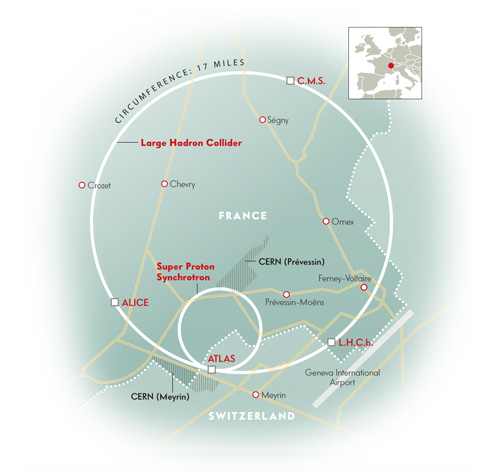
\includegraphics[width=0.99\textwidth]{figures/ch_higgs/misc/lhcring.jpg}
    }
    \caption{LHC Accelerator Complex}
    \label{fig:higgs_cms_lhc}
 \end{figure}

 The Large Hadron Collider is the particle accelerating and colliding complex located on the border between France and Switzerland. Physically speaking, it is a ring that is about 27 km in circumference and serves four major High Energy Physics Experiments: CMS, Atlas, Alice and LHCb.

\subsection{General Description} \label{subsection:higgs_cms_generaldescription}
The Compact Muon Solenoid is a two-fold creature; first of all, it is, a one of its kind, general purpose particle detector system, which consists of multiple components (to be discussed futher) and whose primary objective is to record and reconstruct physics events that could help us study the fundamental building blocks of nature. It acts like a camera, recording the footprint of the physics interactions which particle physicists use to deduce the underlying physics. The Compact Muon Solenoid is also an experiment, a collaboration of thousands of people whose combined effort made it possible to build such a device. From people involved in data-taking at Point 5 and detector maintainance experts to people performing the analysis of recorded events and making sure that the data we have collected is of the highest quality - it is one of the best examples when group effort produces results of highest estime.

The most important component of CMS that makes it stand out among other experiments is the superconducting solenoid with magnetic field of 3.8 T. The magnet is located just outside of HCAL subsystem and plays a crucial role in the overall architecture of CMS. In particular, due to the strength of magnetic field, significant improvements are expected in the search for the Higgs Boson decaying via two muons due to a high resolution of the muon system together with the power of the magnet. The closest subsystem of CMS to the interaction point is the Silicon Tracker, whose primary objective is to measure the trajectory of the charged particles passsing through. What follows are Electromagnetic and Hadronic subsystems which respectively consist of several subdetectors with varying performance characteristics. Muon Systems are located just outside of the magnet and comprise different technologies depending on the $\eta$ location.

The Large Hadron Collider is not just a challenging project from an engineering standpoint, it is also a data factory, one of its kind, that presents a unique challenge for the data processing and analysis domain. The amount of data that gets generated quickly becomes unmanagable and one has to be careful when selecting what to preserve and what to abandon. The collsion rate is about 40 MHz and the compressed size of just 1 event coming from CMS is on order of 1 KB. That amounts to 40 GB/s and if we extrapolate up to a single hour of datataking we get about 140 TB/h - obviously this becomes unfeasible very quickly. For the purpose of selection of events of interest, all HEP Experiments employ a sophisticated Trigger System, whose purpose is to select the physics events of interest. CMS has two layers of data reduction: Level 1 and High Level Trigger. Level 1 trigger system is a hardware based processing system, that is tightly integrated with the rest of the subsystems' electronics. Level 1 allows CMS to reduce the event rate from 40 MHz down to 100 KHz. This is achieved by applying basic selections at hardware level (integration with the subsystems' electronics results in zero copy processing) using reduced content information known as Trigger Primitives (TPs).

The 100 KHz output of Hardware Trigger System gets further reduced by High Level Trigger (HLC) down to 100 Hz that gets actually written to disk. This content reduction is achieved by employing high level information produced via the reconstruction procedure. Basically, CMS High Level Trigger System is a reasonable-sized High Perfomance Cluster (HPC) Complex which takes the output of Level 1 and acts as a filtering system, flagging events that should be stored to disk for offline processing. The software framework that gets used is the same one as for offline data analysis, however certain reconstruction steps are optimized for performance.

%\subsection{Tracker System} \label{subsection:higgs_cms_tracker}
%Explain Pixels and Tracker

%\subsection{Electromagnetic Calorimeter} \label{subsection:higgs_cms_em}
%Electromagnetic Calorimeter (or Ecal for breivity) is a subsystem of CMS with the primary objective to

%\subsection{Hadronic Calorimeter} \label{subsection:higgs_cms_hcal}
%Hadron Calorimeter (or Hcal for breivity) is a subsystem of CMS with the primary objective to identify and measure energy of jets. It consists of four separate parts: Hadron Barrel, Hadron Endcap, Hadron Outer and Hadron Forward.

%\subsection{Muon System} \label{subsection:higgs_cms_muon}
%Describe the Muon Systems

%\subsection{Trigger System} \label{subsection:higgs_cms_trigger}

%\subsection{Data Acquisition Software}

%\subsection{Data Analysis Software} \label{subsection:higgs_cms_cmssw}
%Describe the Software for Analysis
\section{CMS Datasets} \label{section:higgs_data}
At CMS, all of the accumulated data is organized in terms of datasets, which can be logically organized into key-value pairs. A key is the name of a dataset, which uniquely identifies it across the rest of the samples (dataset and sample are used interchangeably). At the same time, a key follows a standard naming convention, which allows to quickly resolve the most important characteristics of the actual data to which it points. A value, in turn, is a collection of data files that actually constitute the dataset and are used for the analysis.

Generally speaking, the CMS experiment produces two types of datasets: collision and simulation samples. Collision samples correspond to the actual data recorded from proton-proton collisions at the LHC. A typical collision sample name has three parts: stream identifier, timestamp and format of the data stored. Depending on the format, timestamp can either point to the actual period of datataking or the reconstruction date. The CMS assigns descriptive stream identifiers in order to provide an overview of the physical content of the events that go into a dataset. For instance, in this search, only events that have a good quality muon object are considered and a ``SingleMuon'' identifier signals exactly that. Furthermore, datasets could have identifiers like ``SingleElectron'' or ``SinglePhoton'', which would make them respectively contain events with an electron or a photon.

Simulation samples correspond to the data produced by simulating the collisions environment (production processes and subsequent decays) and the response of the CMS detector. The most important use case of the simulation is to provide a modeling baseline with which collisions data will be compared. For the purpose of the search, simulation datasets can be further divided into the signal and background samples. Signal corresponds to the Higgs Boson production processes with its subsequent decay to two muons. Backgrounds, in turn, are basically all of the processes that can produce the same signature, the same final state. A typical unique simulation sample name, similar to collision sample name, has three parts: production process specifier, conditions identifier and the format of the data stored. The first part specifies a label that summarizes the actual production process and the Monte Carlo event generators used to perform the calculations of the Feynman diagrams. Conditions part carries a label to uniquely specify a campaign when a sample is produced, software versions used, and various calibrations and corrections applied.

\subsection{Collision Datasets}
For the purpose of the search, datasets with the total integrated luminosity of 35.9 fb$^{-1}$ of CMS collision data collected over the course of 2016 datataking campaign are utilized and the full list of these samples is provided in the Table~\ref{table:higgs_data_collisiondatasets}. The signature of the search is the presence of two opposite sign muons in the event; therefore, in order to pick up as many as possible events of interest, the choice for the stream identifier is limited to either ``SingleMuon'' or ``DoubleMuon''. The choice of ``SingleMuon'' is dictated by the fact of having intrinsically higher efficiency of triggering a single muon rather than two muons per a given event. By selecting ``DoubleMuon'' trigger, for this particular search, all the events where only one muon triggers the HLT system would be thrown away. Therefore, considering that dimuon final state has a very low branching fraction for the Higgs Boson, the choice is made not to throw away the events.
\begin{table}[htb]
    \caption{Datasets used for the search from proton-proton collisions recorded at the $\sqrt{s}=13$~TeV by CMS at LHC in 2016.}
    \label{table:higgs_data_collisiondatasets}
    \begin{center}
        \begin{tabular}{ l  c}
            \hline
            Datasets & Int. Luminosity (fb$^{-1}$)\\
            \hline
            {/SingleMuon/Run2016B-03Feb2017\_ver2-v2/MINIAOD} & 5.788\\
            {/SingleMuon/Run2016C-03Feb2017-v1/MINIAOD} & 2.573\\
            {/SingleMuon/Run2016D-03Feb2017-v1/MINIAOD} & 4.248\\
            {/SingleMuon/Run2016E-03Feb2017-v1/MINIAOD} & 4.009\\
            {/SingleMuon/Run2016F-03Feb2017-v1/MINIAOD} & 3.102\\
            {/SingleMuon/Run2016G-03Feb2017-v1/MINIAOD} & 7.540\\
            {/SingleMuon/Run2016H-03Feb2017\_ver2(3)-v1/MINIAOD} & 8.606\\
            \hline
        \end{tabular}
    \end{center}
\end{table}

\subsection{Signal Datasets}
For the purpose of testing various hypothetical Standard Model Higgs Boson masses, it is crucial to be able to build signal models for each hypothesis. In this analysis, samples with three different hypothetical Higgs Boson masses are used, 120/125/130 GeV, which allows a mass range [120, 130] GeV to be examined. The process of signal model construction and interpolation of parameters as a function of the Higgs Boson mass is discussed in further detail in Section~\ref{section:higgs_signalmodel}. The choice of the mass range is driven by the evidence obtained from searches for the Higgs Boson in other final states, discussed in Section~\ref{section:higgs_run1results}, where observations of a resonance near 125 GeV mass were made. Table~\ref{table:higgs_data_signaldatasets} provides a summary of the CMS signal samples used along with cross section of each production process for the 125 GeV mass hypothesis.
\begin{table}[htb]
    \caption{Standard Model 125 GeV Higgs Boson Signal Datasets for 13 TeV. Dataset names for 120/130 GeV are omitted for brevity. Moriond 2017 conditions are used (omitted the conditions specification for brevity).}
    \label{table:higgs_data_signaldatasets}
        \begin{center}
        \begin{tabular}{ l  c}
            \hline
            Datasets & $\sigma$ (pb)\\
            \hline
            {/GluGlu\_HToMuMu\_M125\_13TeV\_powheg\_pythia8} & 48.58\\
            {/VBF\_HToMuMu\_M125\_13TeV\_powheg\_pythia8} & 3.782\\
            {/WMinusH\_HToMuMu\_M125\_13TeV\_powheg\_pythia8} & 0.5331\\
            {/WPlusH\_HToMuMu\_M125\_13TeV\_powheg\_pythia8} & 0.851\\
            {/ZH\_HToMuMu\_M125\_13TeV\_powheg\_pythia8} & 0.8839 \\
            \hline
        \end{tabular}
        \end{center}
\end{table}
The Higgs signal production processes considered in this search are gluon
fusion (ggH), vector boson fusion (VBF), Higgsstrahlung (VH). Production in
association with top quarks (\ttH) has been generated privately. The Higgs MC samples are generated using {\sc POWHEG}~\cite{Nason:2004rx}.

\subsection{Background Datasets}
As it has already been stated, background processes are the processes that result in the same final state (at least two muons in the event) as the Higgs Boson samples considered. For this analysis, all the processes that produce two muons in the final state, but not through their coupling to the Higgs field,  are to be considered backgrounds. Table~\ref{table:higgs_data_backgrounddatasets} provides a summary of the most dominant contributions among the background processes. The largest contributor is the Drell-Yan process, which constitutes approximately 90\% of background events, and has a pair of leptons in the final state. The next-to-leading contributor is the $\mathrm{t\bar{t}}$ production, with subsequent decay of top quarks into lighter bottom quarks and W$^{\pm}$ vector bosons further coupling to two fermions. These two mechanisms are responsible for more than 98\% of background events contributing to the dimuon final state.
\begin{table}[htb]
    \caption{Background Datasets. Moriond 2017 conditions have been used (omitted the conditions specification for brevity).}
    \label{table:higgs_data_backgrounddatasets}
    \begin{center}
        \begin{tabular}{ l  c}
            \hline
            Dataset & $\sigma$ (pb)\\
            \hline
            /DYJetsToLL\_M-50\_TuneCUETP8M1\_13TeV-amcatnloFXFX-pythia8 & 5765\\
            /ST\_tW\_top\_5f\_NoFullyHadronicDecays\_13TeV-powheg\_TuneCUETP8M1 & 35.85\\
            /TTJets\_DiLept\_TuneCUETP8M1\_13TeV-madgraphMLM-pythia8 & 85.656\\
            /WJetsToLNu\_TuneCUETP8M1\_13TeV-amcatnloFXFX-pythia8 & 61526.7\\
            /WWTo2L2Nu\_13TeV-powheg-herwigpp & 10.481\\
            /WZTo3LNu\_TuneCUETP8M1\_13TeV-amcatnloFXFX-pythia8 & 4.712\\
            \hline
        \end{tabular}
    \end{center}
\end{table}

Depending on the analysis strategy, the role of background simulation samples can be two fold. First, they are used for comparison with collision data, in particular to make sure that dimuon mass is well-modeled by the included backgrounds. The idea is to show that physical quantities of interest (dimuon mass, various kinematic variables) are in line with theoretical predictions. It is important to point out that both data and simulated samples will be further subject to exactly the same selections, further described in Section~\ref{section:higgs_selections}. Second, background datasets can be directly used for the hypothesis testing and statistical analysis of the presence of the signal in the data. In such a case, it is common to abbreviate this approach as simulation driven, because the simulated background dimuon mass distributions are directly used in the hypothesis testing. Another approach, commonly named data driven, is to build a model, similar to the construction of a signal model and discussed further in Section~\ref{section:higgs_bkgmodel}, that will be fit to the actual data, constrained and used to estimate the background yield.

This analysis follows a data-driven background estimation approach due to the low statistical power of simulated background samples. In other words, significant bin-to-bin fluctuations are present, especially for the categories with lower statistics, that would result in inadequate extraction of the upper limits. Therefore, the primary use of background datasets is to compare various kinematic variable distributions from data and theoretical predictions. Moreover, as it will be clarified in Section~\ref{section:higgs_categorization}, depending on the categorization technique used, background samples will be further used for training a binary classification algorithm for the purpose of signal discrimination.

Single top samples are generated with {\sc POWHEG}, whereas $\mathrm{t\bar{t}}$ samples and the multi-boson samples are generated either with {\sc madgrapgh}~\cite{Alwall:2011uj} or {\sc amc@NLO} (Next to Leading Order)~\cite{amcatnlo}. Spin effects in multiboson processes are simulated using {\sc Madspin}. The parton shower and hadronization processes are modeled by the {\sc Pythia8} generator~\cite{Sjostrand:2007gs} with TuneCUETP8M1.

%The simulated pile up distribution is reweighted to match the observed
%distribution in data for all MC samples.

% \begin{table}[!h]
% \small
% \renewcommand{\arraystretch}{1.5}

% \begin{tabular}{|l||l|c|}
%     \hline \textbf{Dataset} & Run Range & Integrated Luminosity \\
%     \hline  &  & [fb$^{-1}$] \\
%     \hline
%         %% %% Fairly certain ver1-v1 is not used at all (no events in Golden JSON - AWB 13.05.16
%     %% \hline \url{/SingleMuon/Run2016B-03Feb2017_ver1-v1/MINIAOD} & \multirow{2}{*}{272007-275376} & \multirow{2}{*}{5.788} \\ \cline{1-1}
%     %% \url{/SingleMuon/Run2016B-03Feb2017_ver2-v2/MINIAOD} &  &  \\
%         \hline \url{/SingleMuon/Run2016B-03Feb2017_ver2-v2/MINIAOD} & 272007-275376 & 5.788 \\
%     \hline \url{/SingleMuon/Run2016C-03Feb2017-v1/MINIAOD}      & 275657-276283 & 2.573 \\
%     \hline \url{/SingleMuon/Run2016D-03Feb2017-v1/MINIAOD}      & 276315-276811 & 4.248 \\
%     \hline \url{/SingleMuon/Run2016E-03Feb2017-v1/MINIAOD}      & 276831-277420 & 4.009 \\
%     \hline \url{/SingleMuon/Run2016F-03Feb2017-v1/MINIAOD}      & 277772-278808 & 3.102 \\
%         \hline \url{/SingleMuon/Run2016G-03Feb2017-v1/MINIAOD}      & 278820-280385 & 7.540 \\
%     \hline \url{/SingleMuon/Run2016H-03Feb2017_ver2-v1/MINIAOD} & \multirow{2}{*}{280919-284044} & \multirow{2}{*}{8.606} \\ \cline{1-1}
%            \url{/SingleMuon/Run2016H-03Feb2017_ver3-v1/MINIAOD} &                                &                        \\
%     \hline                                                         %% Adds up to 35.866 - i.e. 35.9 fb^-1
%     \hline \multicolumn{3}{|l|}{\textbf{Luminosity mask: \url{Cert_271036-284044_13TeV_23Sep2016ReReco_Collisions16_JSON.txt}}}    \\
% \hline
% \end{tabular}

% \caption{Overview of the single muon data stream collected during the
% proton-proton collisions at $\sqrt{s}=13$~TeV by CMS at LHC in 2016.}
% \label{tab:datasets}
% \end{table}

% \newpage
% \begin{landscape}
% \begin{table}[p]
% \renewcommand{\arraystretch}{1.5}
% \tiny
% \begin{tabular}{|l||c|c|c|}
%   \hline \textbf{Higgs signal MC samples} & Events & Cross section [pb] & Xsec $\times$ BR [fb]  \\
%   %% From Yellow Report 4 (https://arxiv.org/abs/1610.07922), H --> mu-mu branching ratio at 125 GeV = 0.0002176
%   %% ggH = 48.58 pb, VBF = 3.7817 pb, W+H = 0.09426 pb, W-H = 0.05983 pb, ZH = 0.17762 pb, ttH = 0.5071 pb
%   \hline
%   \hline \url{/GluGlu_HToMuMu_M125_13TeV_powheg_pythia8/RunIISummer16MiniAODv2-PUMoriond17_80X_mcRun2_asymptotic_2016_TrancheIV_v6-v1/MINIAODSIM }  &  250000 & 48.58    & 10.571   \\
%   \hline \url{/VBF_HToMuMu_M125_13TeV_powheg_pythia8/RunIISummer16MiniAODv2-PUMoriond17_80X_mcRun2_asymptotic_2016_TrancheIV_v6-v1/MINIAODSIM }     &  249200 &  3.7817  & 0.8229   \\
%   \hline \url{/WPlusH_HToMuMu_M125_13TeV_powheg_pythia8/RunIISummer16MiniAODv2-PUMoriond17_80X_mcRun2_asymptotic_2016_TrancheIV_v6-v1/MINIAODSIM }  &  124547 &  0.09426 & 0.02051  \\
%   \hline \url{/WMinusH_HToMuMu_M125_13TeV_powheg_pythia8/RunIISummer16MiniAODv2-PUMoriond17_80X_mcRun2_asymptotic_2016_TrancheIV_v6-v1/MINIAODSIM } &  125000 &  0.05983 & 0.013019 \\
%   \hline \url{/ZH_HToMuMu_M125_13TeV_powheg_pythia8/RunIISummer16MiniAODv2-PUMoriond17_80X_mcRun2_asymptotic_2016_TrancheIV_v6-v1/MINIAODSIM }      &  249748 &  0.17762 & 0.03865  \\
%   %% \hline \url{/ttHToNonbb_M125_TuneCUETP8M2_ttHtranche3_13TeV-powheg-pythia8/RunIISummer16MiniAODv2-PUMoriond17_80X_mcRun2_asymptotic_2016_TrancheIV_v6-v1/MINIAODSIM } & 3981250 & 0.5071 & 0.11034 \\

% \hline
% \end{tabular}

% \caption{The Higgs signal MC samples were generated with {\sc POWHEG}
% while the parton shower and hadronization processes are modeled by the
% {\sc Phythia8} generator with TuneCUETP8M1.}
% \label{tab:SignalMC}
% \end{table}
% \end{landscape}

% \newpage
% \begin{landscape}
% \begin{table}[p]
% \tiny
% \renewcommand{\arraystretch}{1.2}
% \begin{tabular}{|l||c|c|}
%     \hline \textbf{Background MC} & Events & Cross Section [pb]  \\
%     \hline
%     \hline \multicolumn{3}{|c|}{\textbf{Drell--Yan}}  \\
%     \hline
%     \hline \url{/DYJetsToLL_M-50_TuneCUETP8M1_13TeV-amcatnloFXFX-pythia8/RunIISummer16MiniAODv2-PUMoriond17_80X_mcRun2_asymptotic_2016_TrancheIV_v6_ext2-v1/MINIAODSIM} &  122055388 & 5765  \\
%     \hline \url{/DYToLL_0J_13TeV-amcatnloFXFX-pythia8/RunIISummer16MiniAODv2-PUMoriond17_80X_mcRun2_asymptotic_2016_TrancheIV_v6_ext1-v1/MINIAODSIM} & 49579613  &  4754\\
%     %% \hline \url{/DYToLL_0J_13TeV-amcatnloFXFX-pythia8/RunIISummer16MiniAODv2-PUMoriond17_backup_80X_mcRun2_asymptotic_2016_TrancheIV_v6-v1/MINIAODSIM} & 44253240  &  4754    \\
%     \hline \url{/DYToLL_1J_13TeV-amcatnloFXFX-pythia8/RunIISummer16MiniAODv2-PUMoriond17_80X_mcRun2_asymptotic_2016_TrancheIV_v6_ext1-v1/MINIAODSIM} & 49902571  & 888.9 \\
%     %% \hline \url{/DYToLL_1J_13TeV-amcatnloFXFX-pythia8/RunIISummer16MiniAODv2-PUMoriond17_backup_80X_mcRun2_asymptotic_2016_TrancheIV_v6-v1/MINIAODSIM} & 41597712  & 888.9 \\
%     \hline \url{/DYToLL_2J_13TeV-amcatnloFXFX-pythia8/RunIISummer16MiniAODv2-PUMoriond17_80X_mcRun2_asymptotic_2016_TrancheIV_v6-v2/MINIAODSIM} & 42324802  & 348.8 \\
%     \hline \url{/DYToLL_2J_13TeV-amcatnloFXFX-pythia8/RunIISummer16MiniAODv2-PUMoriond17_80X_mcRun2_asymptotic_2016_TrancheIV_v6_ext1-v1/MINIAODSIM} & 47974554  & 348.8 \\
%     %% \hline \url{/DYJetsToLL_M-100to200_TuneCUETP8M1_13TeV-amcatnloFXFX-pythia8/RunIISummer16MiniAODv2-PUMoriond17_80X_mcRun2_asymptotic_2016_TrancheIV_v6_ext1-v1/MINIAODSIM} &  1083606 &  ??? \\
%     \hline
%     \hline \multicolumn{3}{|c|}{\textbf{SingleTop}}    \\
%     \hline
%     \hline \url{/ST_tW_top_5f_NoFullyHadronicDecays_13TeV-powheg_TuneCUETP8M1/RunIISummer16MiniAODv2-PUMoriond17_80X_mcRun2_asymptotic_2016_TrancheIV_v6-v1/MINIAODSIM} & 5372991  & 35.85 \\
%     \hline \url{/ST_tW_top_5f_NoFullyHadronicDecays_13TeV-powheg_TuneCUETP8M1/RunIISummer16MiniAODv2-PUMoriond17_80X_mcRun2_asymptotic_2016_TrancheIV_v6_ext1-v1/MINIAODSIM} & 3256650  & 35.85 \\
%     \hline \url{/ST_tW_antitop_5f_NoFullyHadronicDecays_13TeV-powheg_TuneCUETP8M1/RunIISummer16MiniAODv2-PUMoriond17_80X_mcRun2_asymptotic_2016_TrancheIV_v6-v1/MINIAODSIM} & 5425134  & 35.85 \\
%     \hline \url{/ST_tW_antitop_5f_NoFullyHadronicDecays_13TeV-powheg_TuneCUETP8M1/RunIISummer16MiniAODv2-PUMoriond17_80X_mcRun2_asymptotic_2016_TrancheIV_v6_ext1-v1/MINIAODSIM} & 3256407 & 35.85 \\
%     \hline
%     \hline \multicolumn{3}{|c|}{\textbf{TopPair}}    \\
%     \hline
%     \hline \url{/TTJets_DiLept_TuneCUETP8M1_13TeV-madgraphMLM-pythia8/RunIISummer16MiniAODv2-PUMoriond17_80X_mcRun2_asymptotic_2016_TrancheIV_v6-v1/MINIAODSIM} & 6094476 & 85.656 \\
%     \hline \url{/TTJets_DiLept_TuneCUETP8M1_13TeV-madgraphMLM-pythia8/RunIISummer16MiniAODv2-PUMoriond17_80X_mcRun2_asymptotic_2016_TrancheIV_v6_ext1-v1/MINIAODSIM} & 24350202  & 85.656 \\
%     \hline \url{/TTJets_Dilept_TuneCUETP8M2T4_13TeV-amcatnloFXFX-pythia8/RunIISummer16MiniAODv2-PUMoriond17_80X_mcRun2_asymptotic_2016_TrancheIV_v6-v1/MINIAODSIM} &  14529280 & 85.656  \\
%     \hline
%     \hline \multicolumn{3}{|c|}{\textbf{DiBoson}}    \\
%     \hline
%     \hline \url{/WWTo2L2Nu_13TeV-powheg/RunIISummer16MiniAODv2-PUMoriond17_80X_mcRun2_asymptotic_2016_TrancheIV_v6-v1/MINIAODSIM } & 1999000  & 12.46  \\
%     \hline \url{/WZTo3LNu_TuneCUETP8M1_13TeV-amcatnloFXFX-pythia8/RunIISummer16MiniAODv2-PUMoriond17_80X_mcRun2_asymptotic_2016_TrancheIV_v6-v1/MINIAODSIM} & 11887464  & 2.113 \\
%     \hline \url{/WZTo2L2Q_13TeV_amcatnloFXFX_madspin_pythia8/RunIISummer16MiniAODv2-PUMoriond17_80X_mcRun2_asymptotic_2016_TrancheIV_v6-v1/MINIAODSIM} & 26517272  &  4.409 \\
%     \hline \url{/ZZTo2L2Nu_13TeV_powheg_pythia8/RunIISummer16MiniAODv2-PUMoriond17_80X_mcRun2_asymptotic_2016_TrancheIV_v6-v1/MINIAODSIM} & 8842475  & 0.564  \\
%     \hline \url{/ZZTo2L2Q_13TeV_amcatnloFXFX_madspin_pythia8/RunIISummer16MiniAODv2-PUMoriond17_80X_mcRun2_asymptotic_2016_TrancheIV_v6-v1/MINIAODSIM} & 15345572  & 3.22 \\
%     \hline \url{/ZZTo4L_13TeV-amcatnloFXFX-pythia8/RunIISummer16MiniAODv2-PUMoriond17_80X_mcRun2_asymptotic_2016_TrancheIV_v6_ext1-v1/MINIAODSIM} &  10709784 & 1.212  \\
%     \hline
%     \hline \multicolumn{3}{|c|}{\textbf{TriBoson}}   \\
%     \hline
%     \hline \url{/WWW_4F_TuneCUETP8M1_13TeV-amcatnlo-pythia8/RunIISummer16MiniAODv2-PUMoriond17_80X_mcRun2_asymptotic_2016_TrancheIV_v6-v1/MINIAODSIM } & 240000   &     0.2086  \\
%     \hline \url{/WWZ_TuneCUETP8M1_13TeV-amcatnlo-pythia8/RunIISummer16MiniAODv2-PUMoriond17_80X_mcRun2_asymptotic_2016_TrancheIV_v6-v1/MINIAODSIM} & 250000  & 0.1651 \\
%     \hline \url{/WZZ_TuneCUETP8M1_13TeV-amcatnlo-pythia8/RunIISummer16MiniAODv2-PUMoriond17_80X_mcRun2_asymptotic_2016_TrancheIV_v6-v1/MINIAODSIM} & 246800  & 0.05565 \\
%     \hline \url{/ZZZ_TuneCUETP8M1_13TeV-amcatnlo-pythia8/RunIISummer16MiniAODv2-PUMoriond17_80X_mcRun2_asymptotic_2016_TrancheIV_v6-v1/MINIAODSIM} & 249237  & 0.01398 \\
%     \hline
%     \hline \multicolumn{3}{|c|}{\textbf{SingleTop+X}}    \\
%     \hline
%     \hline \url{/tZq_ll_4f_13TeV-amcatnlo-pythia8/RunIISummer16MiniAODv2-PUMoriond17_80X_mcRun2_asymptotic_2016_TrancheIV_v6_ext1-v1/MINIAODSIM } & 14509520  & 0.0758  \\
%     %\hline \url{/ST_tWll_5f_LO_13TeV-MadGraph-pythia8/RunIISummer16MiniAODv2-PUMoriond17_80X_mcRun2_asymptotic_2016_TrancheIV_v6-v1/MINIAODSIM} &  50000 & ??? \\
%     \hline
%     \hline \multicolumn{3}{|c|}{\textbf{Top pairs}}    \\
%     \hline
%     \hline \url{/TTWJetsToLNu_TuneCUETP8M1_13TeV-amcatnloFXFX-madspin-pythia8/RunIISummer16MiniAODv2-PUMoriond17_80X_mcRun2_asymptotic_2016_TrancheIV_v6_ext1-v3/MINIAODSIM     } & 2160168  & 0.2043 \\
%     \hline \url{/TTWJetsToLNu_TuneCUETP8M1_13TeV-amcatnloFXFX-madspin-pythia8/RunIISummer16MiniAODv2-PUMoriond17_80X_mcRun2_asymptotic_2016_TrancheIV_v6_ext2-v1/MINIAODSIM} & 3120397  & 0.2043 \\
%     \hline \url{/TTZToLLNuNu_M-10_TuneCUETP8M1_13TeV-amcatnlo-pythia8/RunIISummer16MiniAODv2-PUMoriond17_80X_mcRun2_asymptotic_2016_TrancheIV_v6_ext1-v1/MINIAODSIM} & 1992438  & 0.2529 \\

% \hline

% \end{tabular}

% \caption{The MC background processes samples were generated with {amc@NLO}.
% {\sc POWHEG} and {\sc madgrapgh}. Spin effects in multi boson processes are
% simulated using  {\sc madspin}. The parton shower and hadronization processes
%  are modeled by the {\sc Phythia8} generator with TuneCUETP8M1.}
% \label{tab:BkgMC}
% \end{table}
% \end{landscape}

%\subsection{Pileup Reweighting}
%\label{pu}

% Each MC samples is reweighted in order to match the pileup distribution in data, as centrally recommended using the ``minimum bias'' cross section of $69.2$mb $\pm5\%$.
% The value needs to be read as an effective minimum bias times efficiesies cross section with respect to what present in pythia8; large uncertainties are present in order to cover differences between the run period and the charge/neutral compenents.

% \begin{figure}[h!]
%     \centering
%     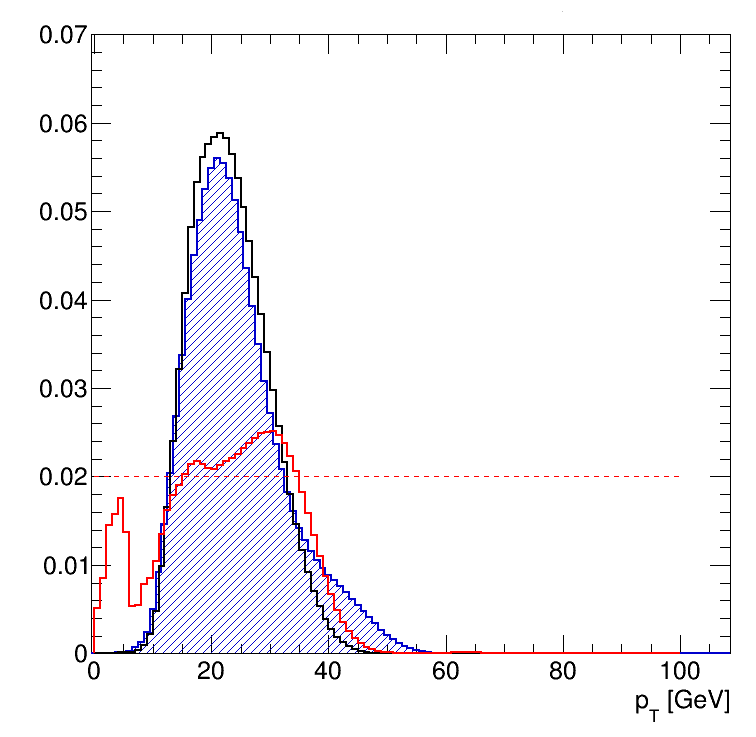
\includegraphics[width=0.49\textwidth]{figures/data_mc_samps/Pu-reweight2.png}
%     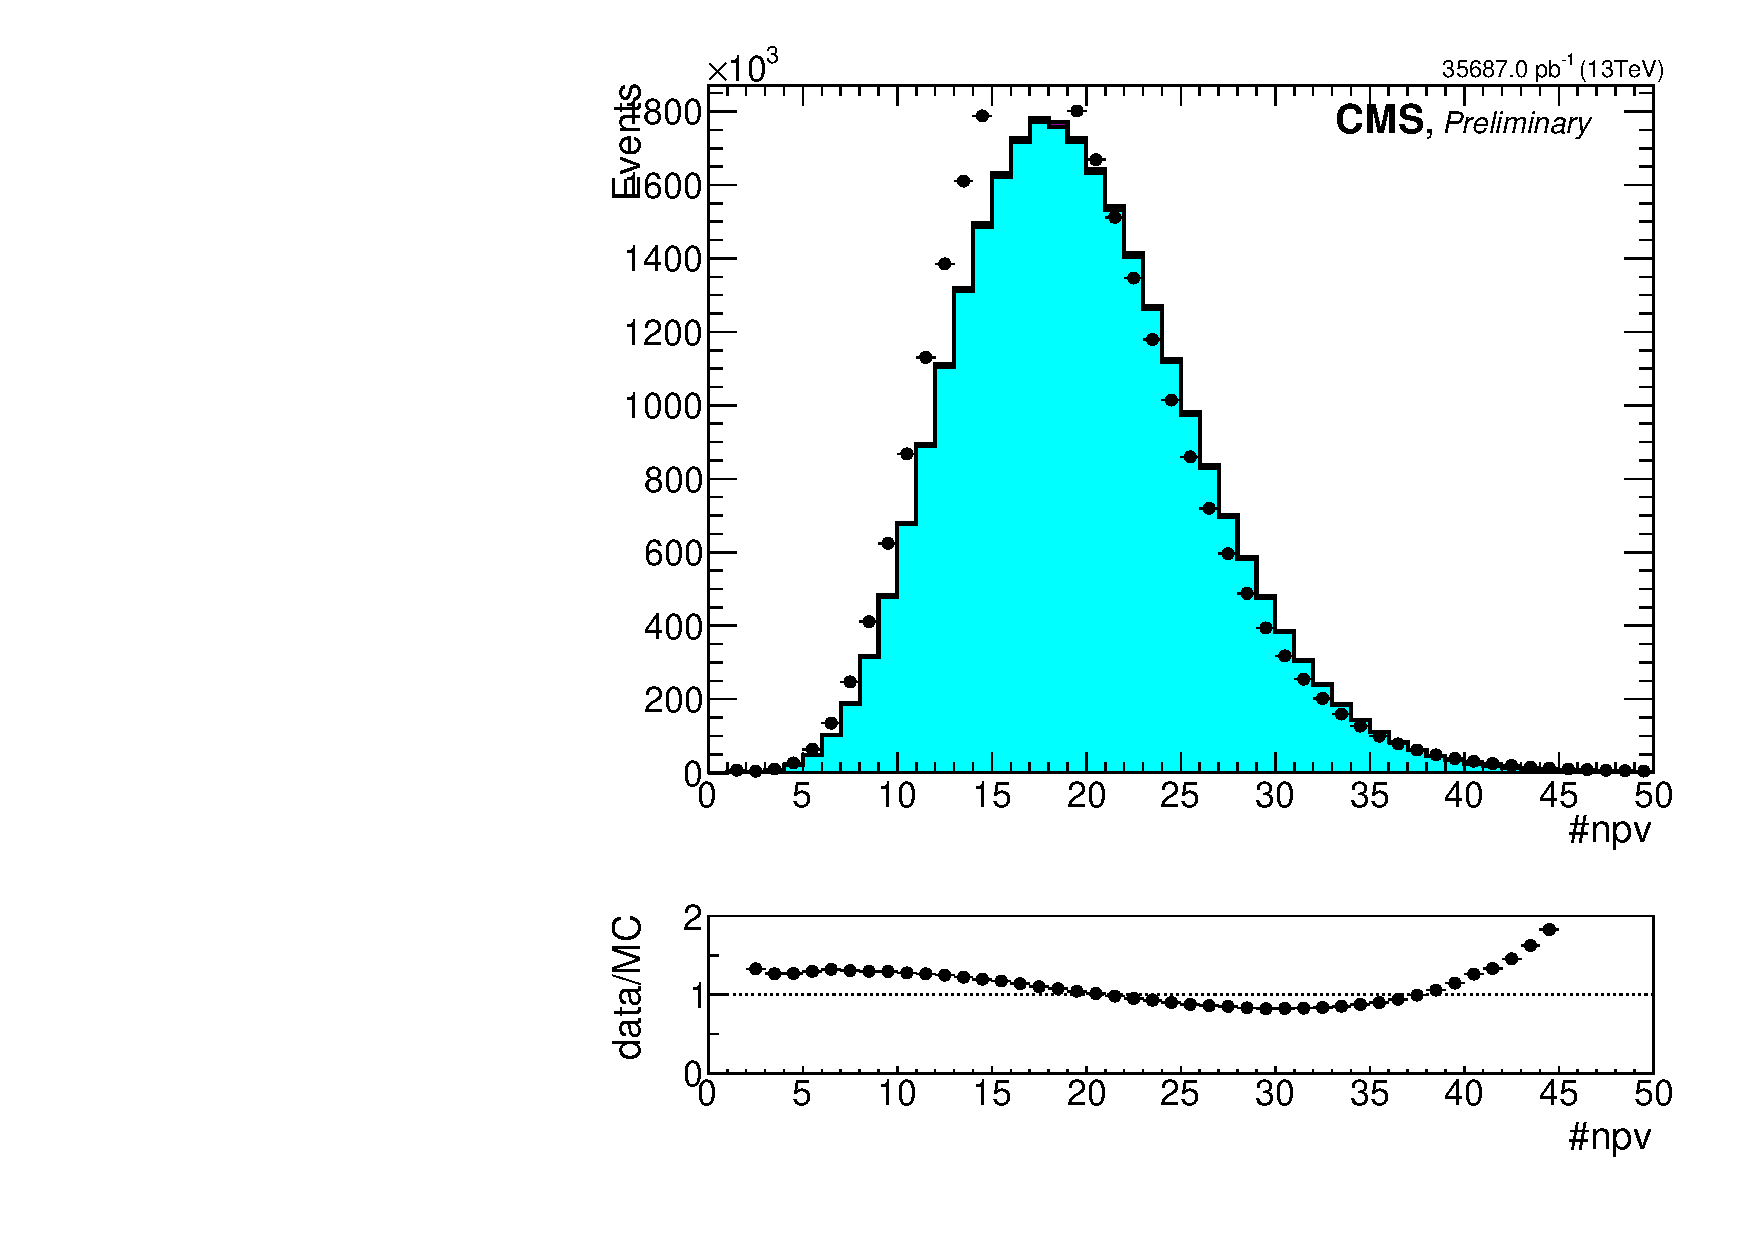
\includegraphics[width=0.49\textwidth]{figures/data_mc_samps/mmNpv_pileup69200.pdf}\\
%     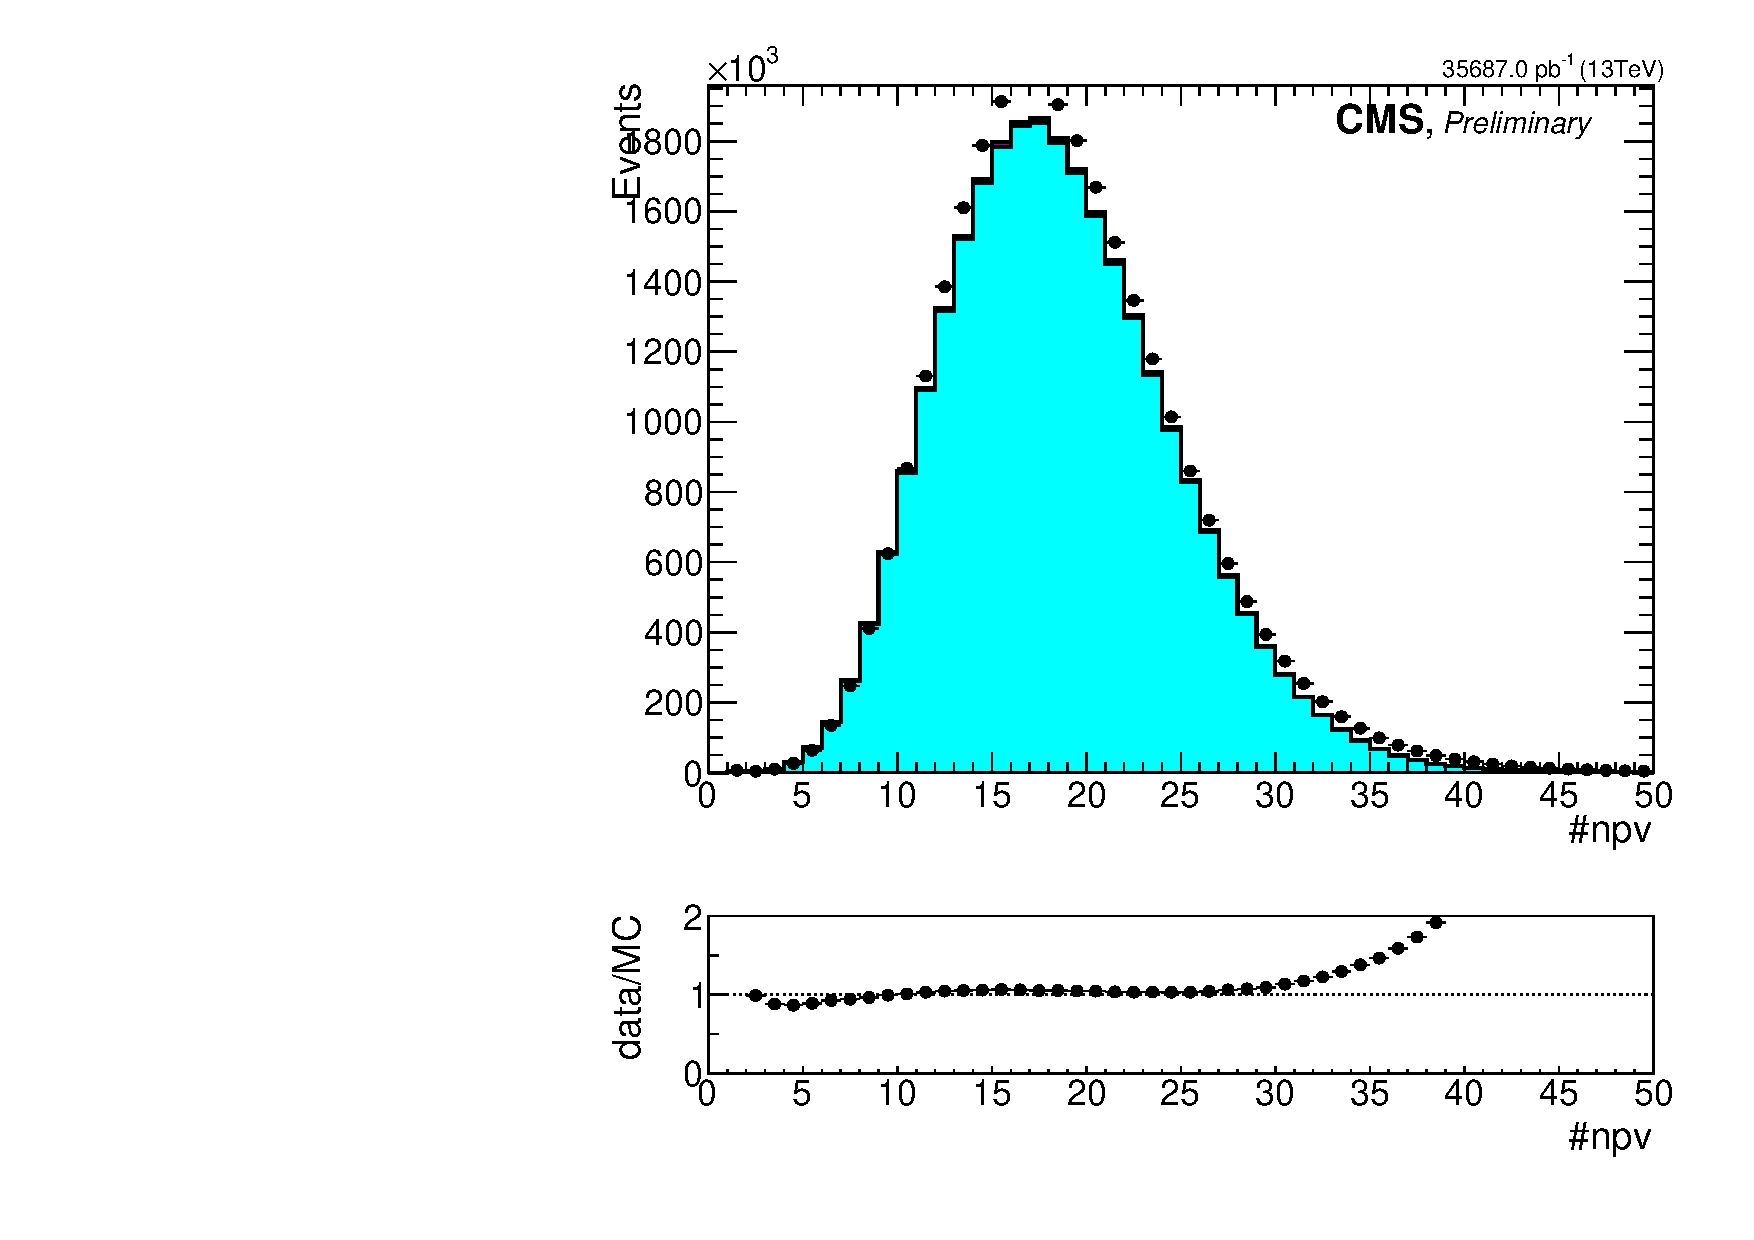
\includegraphics[width=0.49\textwidth]{figures/data_mc_samps/mmNpv_pileup65000.pdf}
%     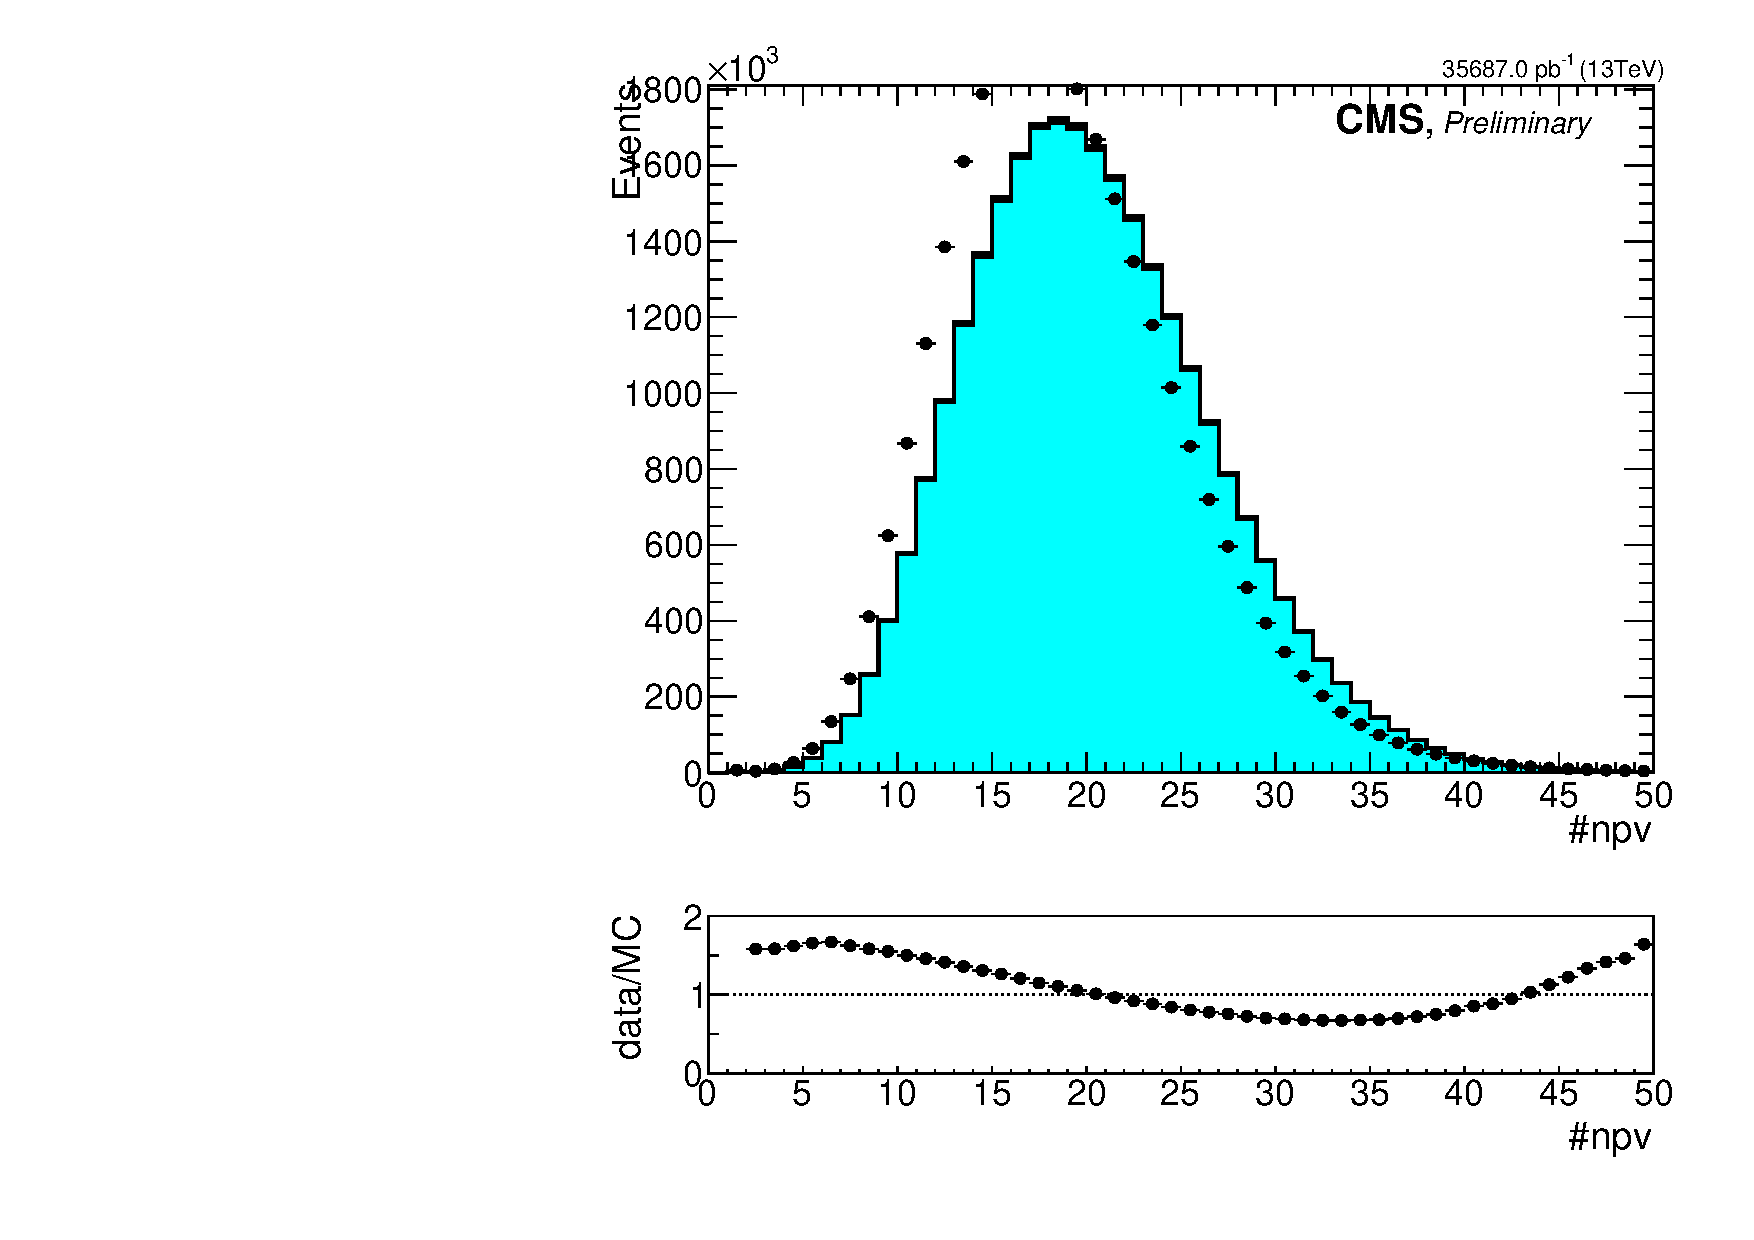
\includegraphics[width=0.49\textwidth]{figures/data_mc_samps/mmNpv_pileup72000.pdf}
%     \caption{Top Left. Pileup reweighting factors, data and MC truth pileup distributions. Top Right. agreement in the number of primary vertex variable after pu-reweighting. Bottom. agreement for the n.p.v. variables after $\pm1\sigma$ uncertainty in the pu-reweighting cress section.}
% \end{figure}




%\section{CMS Monte-Carlo Datasets} \label{section:higgs_mc}


\subsection{Signal Samples} \label{subsection:higgs_mc_signal}
We use Signal Samples with three different hypothetical Standard Model Higgs Boson masses. Since we are performing a search and are leaving the mass floating, we need a way to probe various hypotheses. Using three mass points (samples) we can model parameters for a given model and further perform interpolation to deduce the parameters for any mass that falls within our range.

\begin{table}[!h]
    \caption{Signal Samples}
    \label{table:higgs_mc_signal}
    \begin{center}
        \begin{tabular}{|l|l|}
            \hline
            Dataset & Mass\\
            \hline
            /GluGlu\_HToMuMu\_M120\_13TeV\_powheg\_pythia8/\\RunIISummer16MiniAODv2-PUMoriond17\_80X\_mcRun2\_asymptotic\_2016\_\\TrancheIV\_v6-v1/MINIAODSIM & 120 GeV\\
            /GluGlu\_HToMuMu\_M125\_13TeV\_powheg\_pythia8/\\RunIISummer16MiniAODv2-PUMoriond17\_80X\_\\mcRun2\_asymptotic\_2016\_TrancheIV\_v6-v1/MINIAODSIM & 125 GeV\\
            /GluGlu\_HToMuMu\_M130\_13TeV\_powheg\_pythia8/\\RunIISummer16MiniAODv2-PUMoriond17\_80X\_mcRun2\_asymptotic\_2016\_\\TrancheIV\_v6-v1/MINIAODSIM & 130 GeV\\
            \hline
            /VBF\_HToMuMu\_M120\_13TeV\_powheg\_pythia8/\\RunIISummer16MiniAODv2-PUMoriond17\_80X\_\\mcRun2\_asymptotic\_2016\_TrancheIV\_v6-v1/MINIAODSIM & 120 GeV\\
            /VBF\_HToMuMu\_M125\_13TeV\_powheg\_pythia8/\\RunIISummer16MiniAODv2-PUMoriond17\_80X\_\\mcRun2\_asymptotic\_2016\_TrancheIV\_v6-v1/MINIAODSIM & 125 GeV\\
            /VBF\_HToMuMu\_M130\_13TeV\_powheg\_pythia8/\\RunIISummer16MiniAODv2-PUMoriond17\_80X\_\\mcRun2\_asymptotic\_2016\_TrancheIV\_v6-v1/MINIAODSIM & 130 GeV\\
            \hline
            /WMinusH\_HToMuMu\_M120\_13TeV\_powheg\_pythia8/\\RunIISummer16MiniAODv2-PUMoriond17\_80X\_\\mcRun2\_asymptotic\_2016\_TrancheIV\_v6-v1/MINIAODSIM & 120 GeV\\
            /WMinusH\_HToMuMu\_M125\_13TeV\_powheg\_pythia8/\\RunIISummer16MiniAODv2-PUMoriond17\_80X\_\\mcRun2\_asymptotic\_2016\_TrancheIV\_v6-v1/MINIAODSIM & 125 GeV\\
            /WMinusH\_HToMuMu\_M130\_13TeV\_powheg\_pythia8/\\RunIISummer16MiniAODv2-PUMoriond17\_80X\_\\mcRun2\_asymptotic\_2016\_TrancheIV\_v6-v1/MINIAODSIM & 130 GeV\\
            \hline
            /WPlusH\_HToMuMu\_M120\_13TeV\_powheg\_pythia8/\\RunIISummer16MiniAODv2-PUMoriond17\_80X\_\\mcRun2\_asymptotic\_2016\_TrancheIV\_v6-v1/MINIAODSIM & 120 GeV\\
            /WPlusH\_HToMuMu\_M125\_13TeV\_powheg\_pythia8/\\RunIISummer16MiniAODv2-PUMoriond17\_80X\_\\mcRun2\_asymptotic\_2016\_TrancheIV\_v6-v1/MINIAODSIM & 125 GeV\\
            /WPlusH\_HToMuMu\_M130\_13TeV\_powheg\_pythia8/\\RunIISummer16MiniAODv2-PUMoriond17\_80X\_\\mcRun2\_asymptotic\_2016\_TrancheIV\_v6-v1/MINIAODSIM & 130 GeV\\
            \hline
            /ZH\_HToMuMu\_M120\_13TeV\_powheg\_pythia8/\\RunIISummer16MiniAODv2-PUMoriond17\_80X\_\\mcRun2\_asymptotic\_2016\_TrancheIV\_v6-v1/MINIAODSIM & 120 GeV\\
            /ZH\_HToMuMu\_M125\_13TeV\_powheg\_pythia8/\\RunIISummer16MiniAODv2-PUMoriond17\_80X\_\\mcRun2\_asymptotic\_2016\_TrancheIV\_v6-v1/MINIAODSIM & 125 GeV\\
            /ZH\_HToMuMu\_M130\_13TeV\_powheg\_pythia8/\\RunIISummer16MiniAODv2-PUMoriond17\_80X\_\\mcRun2\_asymptotic\_2016\_TrancheIV\_v6-v1/MINIAODSIM & 130 GeV\\
            \hline
        \end{tabular}
    \end{center}
\end{table}

\subsection{Background Samples} \label{subsection:higgs_mc_background}
Table~\ref{table:higgs_mc_background} provides a summary of the most dominant contributions among the background processes. Given that we use data-driven approach for our search, background samples are not used in any of the statistical modeling. However, the primary use of background datasets is to compare various kinematic variable distributions from data and theoretical predictions in section~\ref{section:higgs_results}

\begin{table}[!h]
    \caption{Background Samples}
    \label{table:higgs_mc_background}
    \begin{center}
        \begin{tabular}{|l|}
            \hline
            Dataset\\
            \hline
            /DYJetsToLL\_M-50\_TuneCUETP8M1\_13TeV-amcatnloFXFX-pythia8/RunIISummer16MiniAODv2-PUMoriond17\_HCALDebug\_80X\_mcRun2\_asymptotic\_2016\_TrancheIV\_v6-v1/MINIAODSIM\\
            /TTJets\_DiLept\_TuneCUETP8M1\_13TeV-madgraphMLM-pythia8/RunIISummer16MiniAODv2-PUMoriond17\_80X\_mcRun2\_asymptotic\_2016\_TrancheIV\_v6-v1/MINIAODSIM\\
            /WJetsToLNu\_TuneCUETP8M1\_13TeV-amcatnloFXFX-pythia8/RunIISummer16MiniAODv2-PUMoriond17\_80X\_mcRun2\_asymptotic\_2016\_TrancheIV\_v6-v1/MINIAODSIM\\
            /WWTo2L2Nu\_13TeV-powheg-herwigpp/RunIISummer16MiniAODv2-PUMoriond17\_80X\_mcRun2\_asymptotic\_2016\_TrancheIV\_v6-v1/MINIAODSIM\\
            /WZTo3LNu\_TuneCUETP8M1\_13TeV-amcatnloFXFX-pythia8/RunIISummer16MiniAODv2-PUMoriond17\_80X\_mcRun2\_asymptotic\_2016\_TrancheIV\_v6-v1/MINIAODSIM\\
            \hline
        \end{tabular}
    \end{center}
\end{table}

\subsection{Pile-Up Reweighting} \label{subsection:higgs_mc_pu}

\section{Event Selections} \label{section:higgs_selections}
For the purpose of reconstruction of physics objects of interest, CMS utilizes Particle Flow Algorithm~\cite{CMS-PAS-PFT-10-002}, which aims to identify individual final state particles: photons, electrons, various hadrons, muons, etc. The main idea behind this algorithm is to use information not just from a particular subsystem (Muon, HCAL, ECAL, Tracker), but to combine and cross-reference features from various subdetectors: hits in the Tracker with Muon Stations, or clusters of energy depositions in ECAL, etc. In other words, this is an example of a sophisticated clusterization technique aimed to improve the reconstruction efficiency.

%For the purpose of our search, given the potential final states, the most important physics objects to be used are muons and jets. On top,

\subsection{Muon Selections}
The muon candidates are reconstructed using the Particle Flow Algorithm by matching compatible track segments from the inner silicon tracker and the muon detectors~\cite{Chatrchyan:2012xi}. In our analysis, we require only muons within the pseudorapidity range $|\eta|<2.4$ and with a minimum transverse momentum $p_{T}>10$ GeV. Furthermore, we require our muon to have $\Delta \beta$-corrected relative isolation, defined in equation~\ref{eq:higgs_selections_isolation}, of $I_{rel}^{PF}<0.25$. In the definition of the isolation variable $p_{T}^{ch}$ is the charged hadron transverse momenta sum, $E_{T}^{\gamma}$ is the photon transverse energy sum, and $E_{T}^{nh}$ is the neutral hadron transverse energy sum. The term $p_{T}^{chPU}$ is the estimated transverse momentum of charged particles from pileup in the $\Delta R < 0.4$, defined in equation~\ref{eq:higgs_selections_deltar}, cone, and the factor of 0.5 is used to estimate the neutral pileup from the charged component.
\begin{center}
   \begin{equation}
      \label{eq:higgs_selections_deltar}
      {\Delta R} = {\sqrt{\Delta\eta^{2}+\Delta\phi^{2}}}
   \end{equation}
\end{center}
\begin{center}
   \begin{equation}
      \label{eq:higgs_selections_isolation}
      {I_{rel}^{PF}} = {(p_{T}^{ch}+max(0,E_{T}^{\gamma}+E_{T}^{nh}-0.5*p_{T}^{chPU}))/p_{T}^{\mu}}
   \end{equation}
\end{center}

Additionally, we only utilize ``Medium Id'' muons~\cite{CMS-MuonPOG}. As we mentioned previously, muons are reconstructed using clusters of hits from various subsystems (Tracker and Muon Stations); in other words we define a physics object Muon to be a composite cluster of combined hits from Tracker and Muon Systems. It's important to understand the difference between actual particles Muons and our definition of a muon! Moreover, when extracting the momentum of a muon, a certain regression procedure is performed, a fit for instance, from which we can extract the goodness of fit or some other quality metric, using which we can judge upon the quality of the reconstructed candidate. Finally, Muon Id is a set of criteria that define a muon candidate of certain quality and allow us to discriminate candidates based on this feature.

\subsection{Muon Corrections}
Given a very narrow theoretical width of the Higgs Boson, around 5 MeV, the Higgs peak is dominated by the Muon detector resolution which is on the order of a GeV. Therefore, to increase the sensitivity of our search, it's crucial to have the best possible dimuon mass resolution, both in data and Monte Carlo. Moreover, as it is going to be described further in the Statistical Modeling sections, we need to correct for possible dimuon mass scale shifts.

There are two different sets of Muon corrections tested: Rochester~\cite{CMS-RochesterCorrections} and Kalman~\cite{CMS-KalmanFilter}. Both allow to correct the scale and smear the resolution. For the validation purposes, we look at the Z peak scale and resolution using these two sets. In Figures~\ref{fig:higgs_selections_zscale}, ~\ref{fig:higgs_selections_zresolution}  comparisons of uncorrected with the two types of corrections are shown for the scale and resolution, respectively. Both the Rochester and Kalman muon corrections successfully align Data with MC in terms of the Z peak.
\begin{figure}[!h]
  \centering
  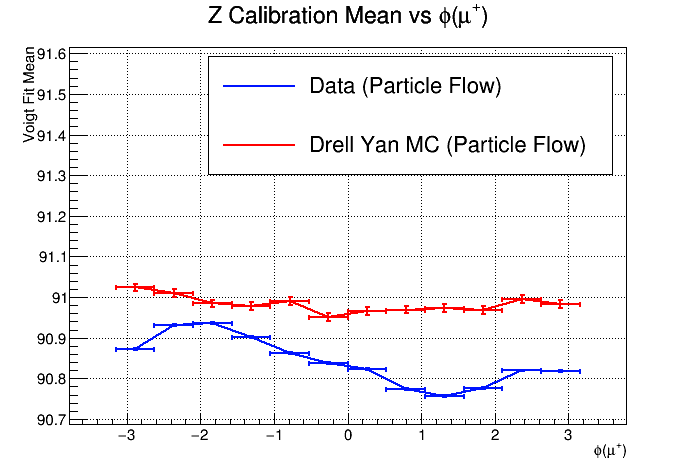
\includegraphics[width=0.32\linewidth]{figures/muon_calib/zcal_pf_mc-data_mean_phi_plus.png}
  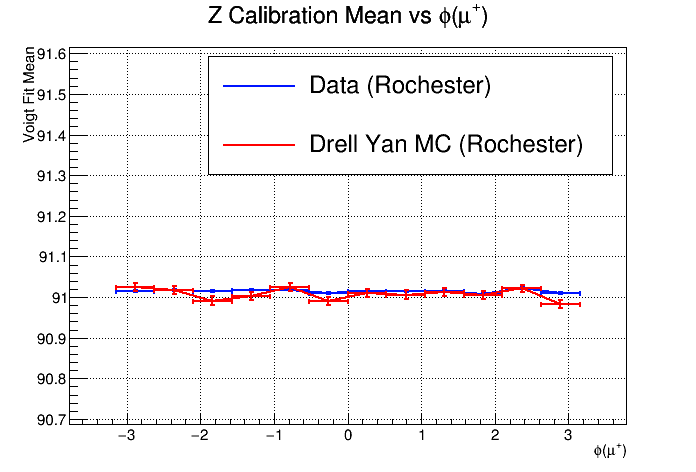
\includegraphics[width=0.32\linewidth]{figures/muon_calib/zcal_roch_mc-data_mean_phi_plus.png}
  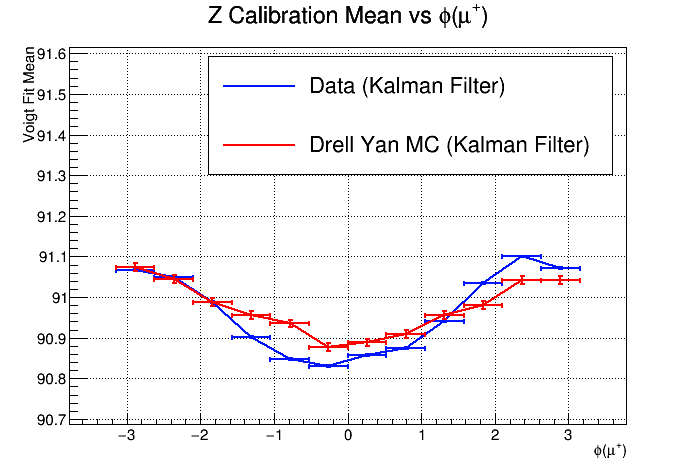
\includegraphics[width=0.32\linewidth]{figures/muon_calib/zcal_kamu_mc-data_mean_phi_plus.png}\\
  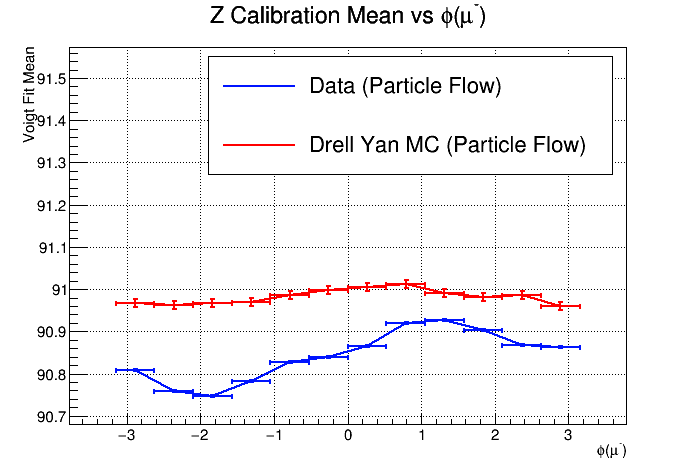
\includegraphics[width=0.32\linewidth]{figures/muon_calib/zcal_pf_mc-data_mean_phi_minus.png}
  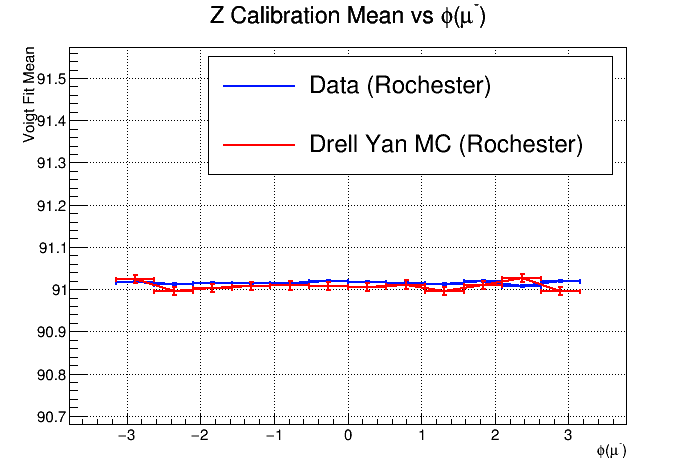
\includegraphics[width=0.32\linewidth]{figures/muon_calib/zcal_roch_mc-data_mean_phi_minus.png}
  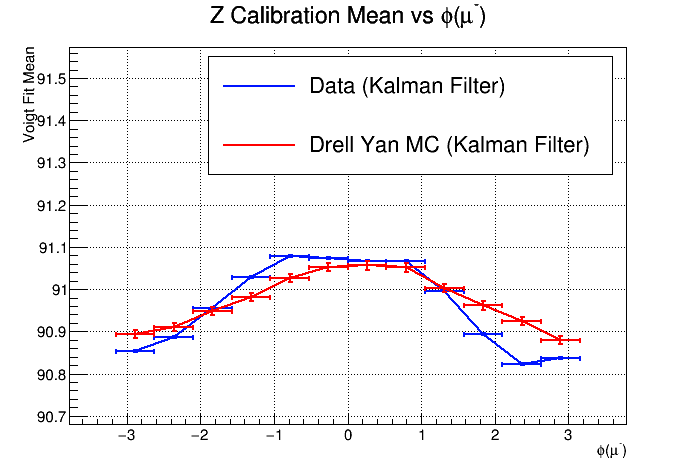
\includegraphics[width=0.32\linewidth]{figures/muon_calib/zcal_kamu_mc-data_mean_phi_minus.png}
  \caption{Comparing Uncorrected (left), Rochester (center) and Kalman (right) Corrections effects on Z Scale.}
  \label{fig:higgs_selections_zscale}
\end{figure}

\begin{figure}[!h]
  \centering
  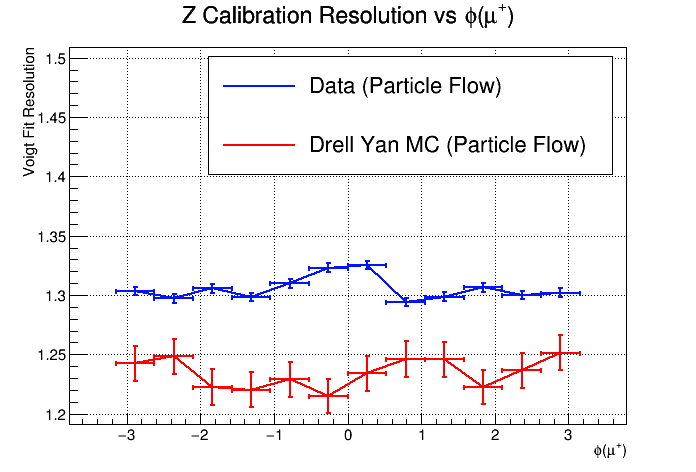
\includegraphics[width=0.32\linewidth]{figures/muon_calib/zcal_pf_mc-data_res_phi_plus.png}
  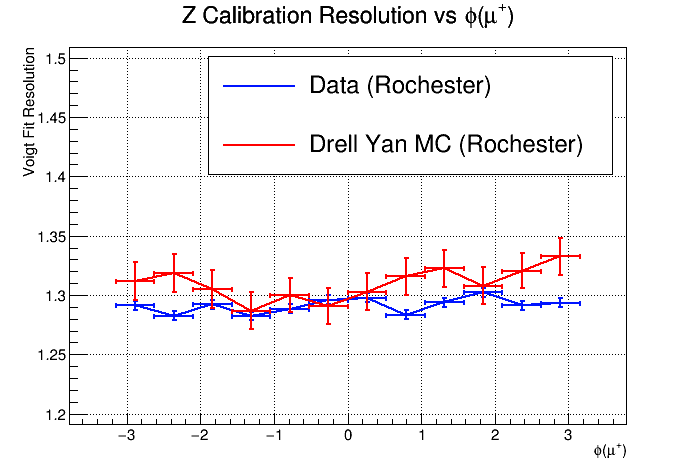
\includegraphics[width=0.32\linewidth]{figures/muon_calib/zcal_roch_mc-data_res_phi_plus.png}
  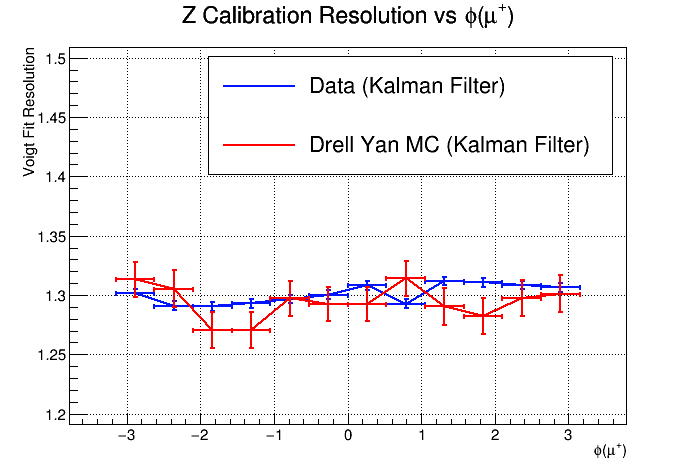
\includegraphics[width=0.32\linewidth]{figures/muon_calib/zcal_kamu_mc-data_res_phi_plus.png}\\
  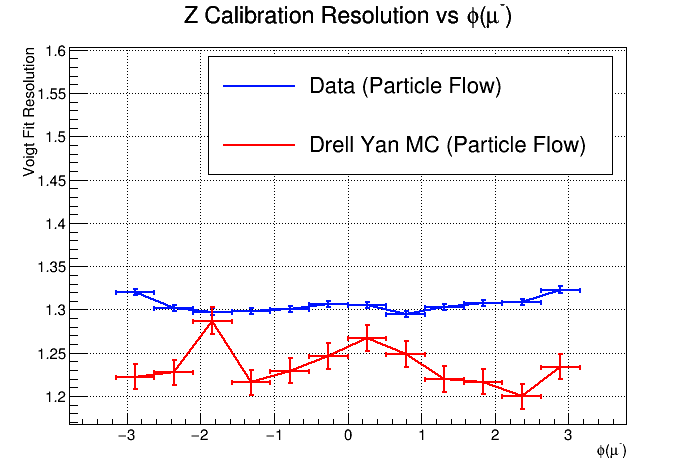
\includegraphics[width=0.32\linewidth]{figures/muon_calib/zcal_pf_mc-data_res_phi_minus.png}
  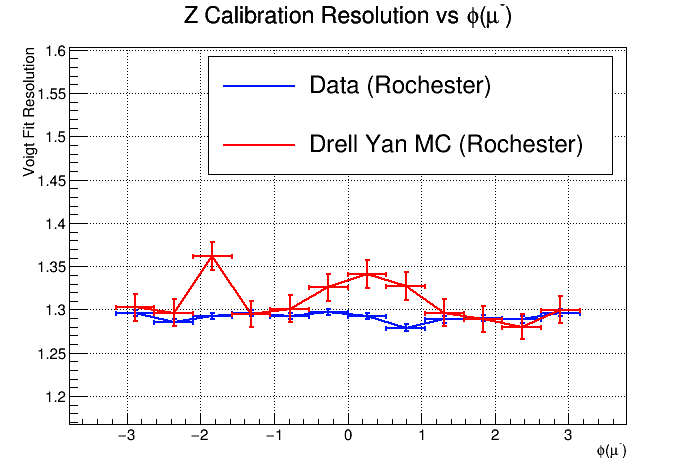
\includegraphics[width=0.32\linewidth]{figures/muon_calib/zcal_roch_mc-data_res_phi_minus.png}
  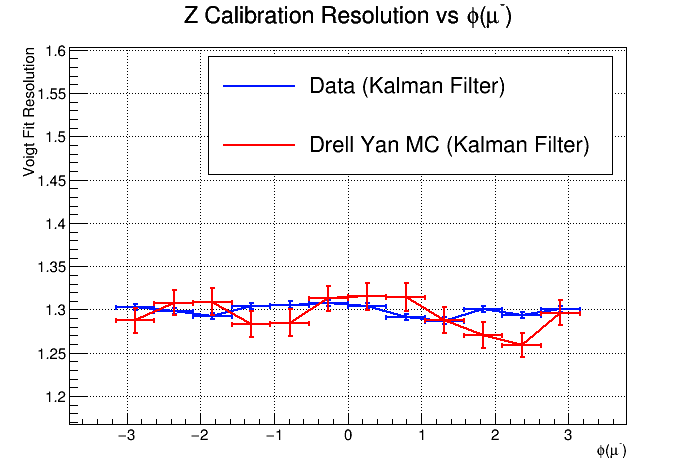
\includegraphics[width=0.32\linewidth]{figures/muon_calib/zcal_kamu_mc-data_res_phi_minus.png}
  \caption{Comparing Uncorrected (left), Rochester (center) and Kalman (right) Corrections effects on Z Resolution.}
  \label{fig:higgs_selections_zresolution}
\end{figure}

\subsection{Jet Selections}
Jets are reconstructed from PF candidates with the anti-$\kappa_{T}$ algorithm~\cite{Cacciari:2008gp} with a distance parameter of 0.4 after rejecting the charged hadrons that are associated to pileup primary vertices. Jets are cleaned against muons - jets overlapping with the selected PF muons, $\Delta R < 0.4$, are not considered further in the analysis. The selected jets with a minimum \pt of 30 GeV and a maximum $|\eta|$ of 4.7 are corrected in energy in order to account for the non-uniform detector response.

The PF jets are further required to fulfill the jet identification criteria.
Candidates with $|\eta|$ less than 2.7 are required to contain at
least one charged PF candidate and have a non-zero charged energy fraction,
and a charged electromagnetic energy fraction less than 0.99. The
neutral and photon energy fraction must be less than 0.99. Jets in
the region $2.7<|\eta|<3.0$ are required to have a neutral electromagnetic
fraction of greater than 0.01 and neutral hadron fraction less than
0.98 while jets with pseudorapidity above 3.0 are required to have more
than 10 neutral particles and a neutral electromagnetic energy fraction
less than 0.9.

For reconstructed jets with $|\eta| < 2.4$, the combined secondary vertex b-tagging algorithm (CSVv2)~\cite{Chatrchyan:2012jua} response is used to discriminate against the $t\bar{t}$ background process events when defining the event categories. The CSVv2 medium operating point is chosen as base line for this analysis and corresponds to a b-tagging efficiency of $60-65\%$ while the misidentification rate for light quarks such as $u$, $d$, $s$, and gluon jets is approximately 1\%.

\subsection{HLT Selections}
Our search requires one of the following Single Isolated Muon Triggers to fire per event:
\begin{itemize}
  \item HLT\_IsoMu24
  \item HLT\_IsoTkMu24
\end{itemize}
The choice of the threshold is driven by the requirement of the lowest \pt threshold to be present during the whole course of datataking. These triggers require the event to have at least one isolated muon candidate with \pt above 24 GeV, with no explicit restriction on its pseudorapidity.

\subsection{Primary Vertex Selection}
One of the top requirements on selecting a proton-proton collision event is the presence of at least 1 valid Primary Vertex with the following conditions:
\begin{itemize}
  \item $ndf \ge 4$ - number of tracks originating from this PV is greater than 4
  \item $\rho < 2$ cm and $|Z| < 24$ cm - displacement along either Z-axis or in the transverse plan should be minimal w.r.t. Interaction Point, defined as (0,0,0).
\end{itemize}

\subsection{Selections Summary}
We can summarize cuts and selections for our search as follows:
\begin{itemize}
  \item At least 1 Primary Vertex passing the PV Selections
  \item At least 1 of the HLT Paths fired
  \item At least 2 opposite sign muons which pass Muon Selections. If more than 1 pair - choose the 2 candidates with the highest \pt. That is the Higgs Candidate.
  \item At least 1 muon from the Higgs Candidate pair with $p_t > 26$ GeV and is matched to the HLT Path that fires the event with $\Delta R < 0.1$.
  \item Filter out the jets that do not pass the Jet Selections, but do not require a certain number of them at this stage.
\end{itemize}

\subsection{Validation}
After applying all of the specified selections, we arrive at a set of events that we are going to further use in order to maximize the sensitivity of our search. However, before proceeding to the next section, we need to validate basic kinematic variables for the inclusive distributions.

First, in the figure~\ref{fig:higgs_selections_inclusivemassnocorr}, inclusive dimuon mass distribution is presented without any muon momentum corrections applied. Notice the presence of a kick near the Z peak. It is the result of a discrepancy in both the mass scale and resolution.
\begin{figure}[!h]
  \centering
  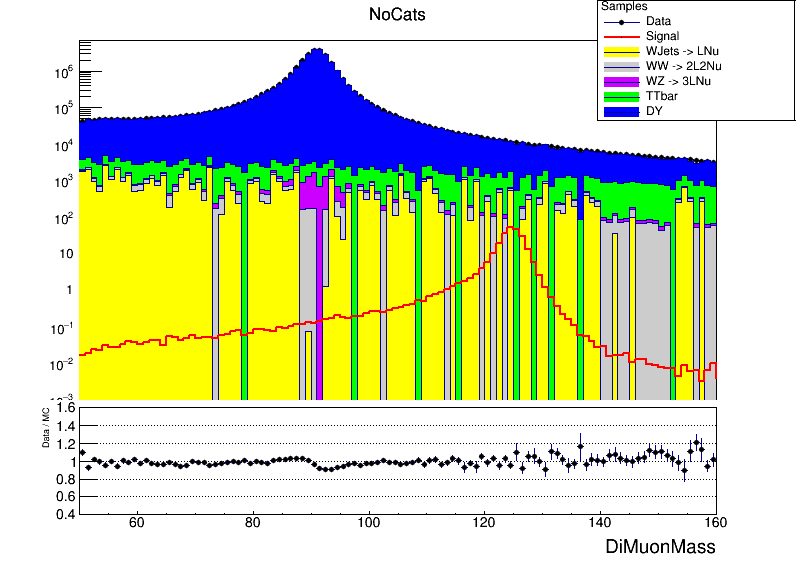
\includegraphics[width=0.5\linewidth]{figures/ch_higgs/distributions/baseline_nocorrections/distribution__NoCats__DiMuonMass__logY.png}
  \caption{Inclusive Dimuon Mass Distributions without any Muon Corrections. Notice the discrepancy around the Z peak}
  \label{fig:higgs_selections_inclusivemassnocorr}
\end{figure}

Second, in the figure~\ref{fig:higgs_selections_inclusivekinematic}, distributions of various kinematic variables after passing the selections are presented.
\begin{figure}[!h]
  \centering
  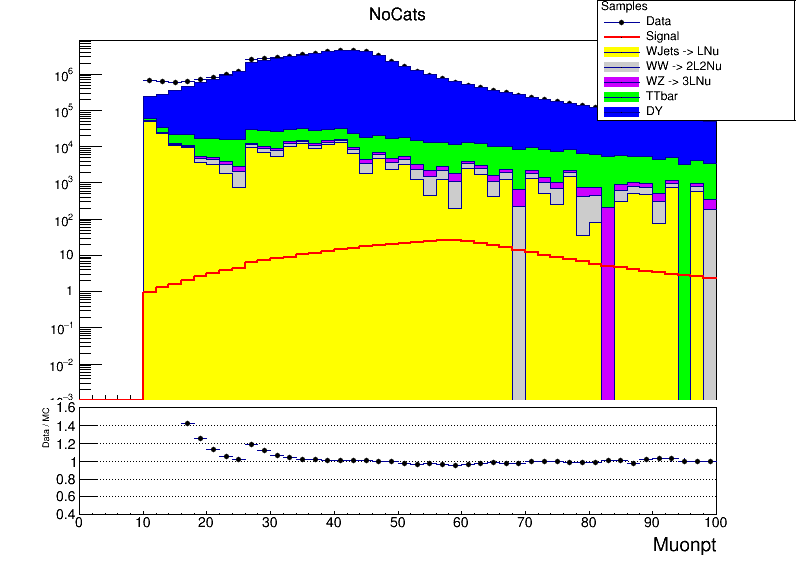
\includegraphics[width=0.45\linewidth]{figures/ch_higgs/distributions/baseline_kalman/distribution__NoCats__Muonpt__logY.png}
  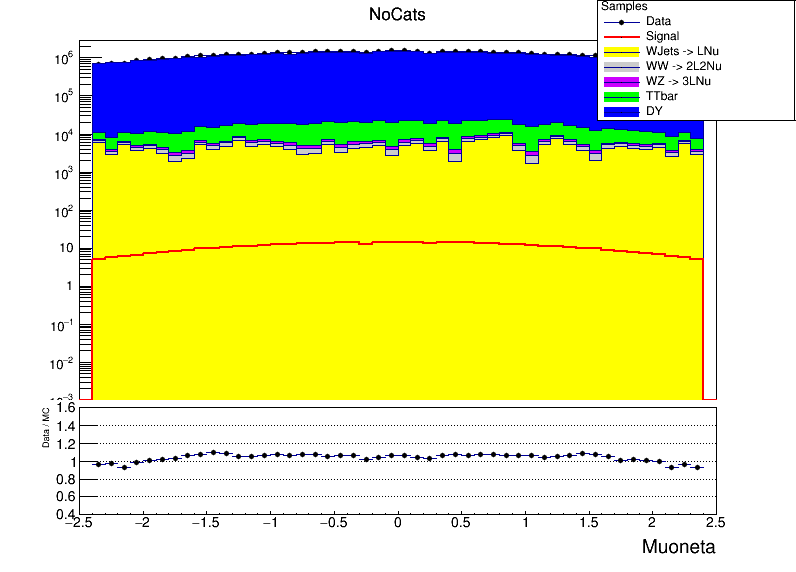
\includegraphics[width=0.45\linewidth]{figures/ch_higgs/distributions/baseline_kalman/distribution__NoCats__Muoneta__logY.png}\\
  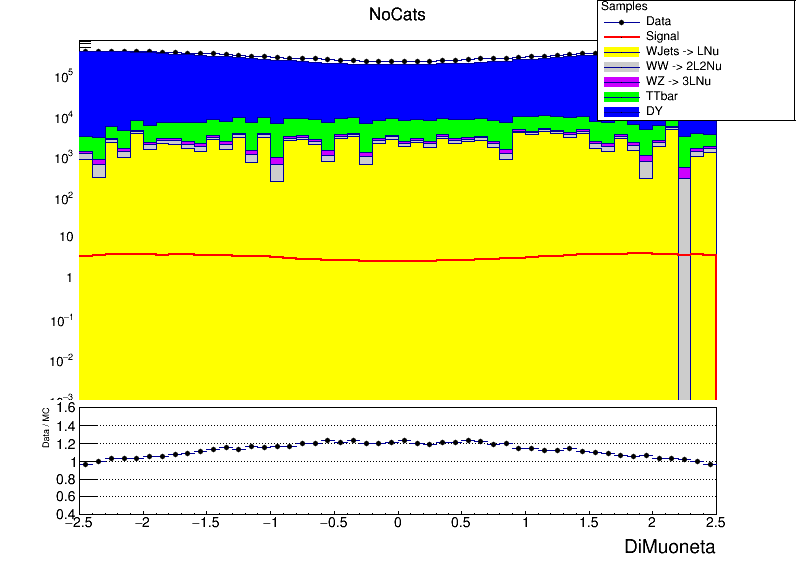
\includegraphics[width=0.45\linewidth]{figures/ch_higgs/distributions/baseline_kalman/distribution__NoCats__DiMuoneta__logY.png}
  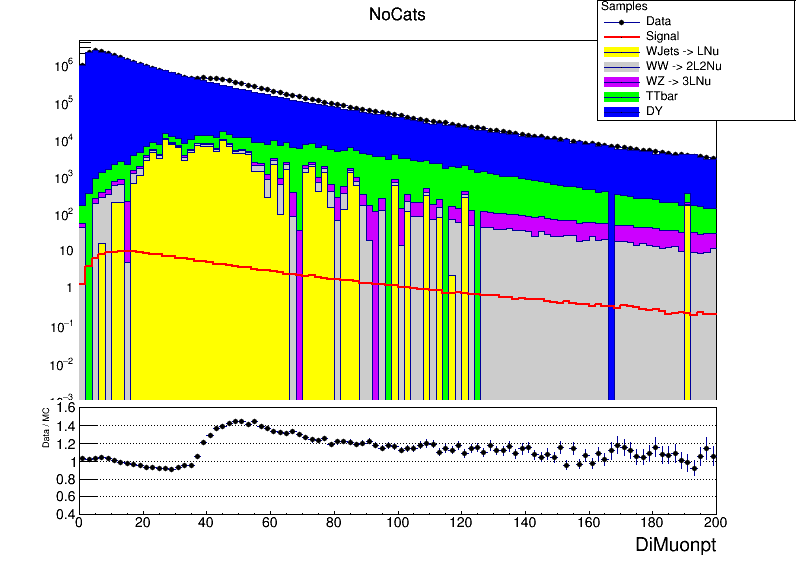
\includegraphics[width=0.45\linewidth]{figures/ch_higgs/distributions/baseline_kalman/distribution__NoCats__DiMuonpt__logY.png}
  \caption{Inclusive Kinematic Distributions.}
  \label{fig:higgs_selections_inclusivekinematic}
\end{figure}

Furthermore, in the figure~\ref{fig:higgs_selections_inclusivemass}, the inclusive dimuon mass distributions are shown with Rochester and Kalman corrections respectively applied to both Data and Monte Carlo. Notice that the discrepancy in scale and resolution is not present anymore around the Z peak.
\begin{figure}[hbp]
  \centering
  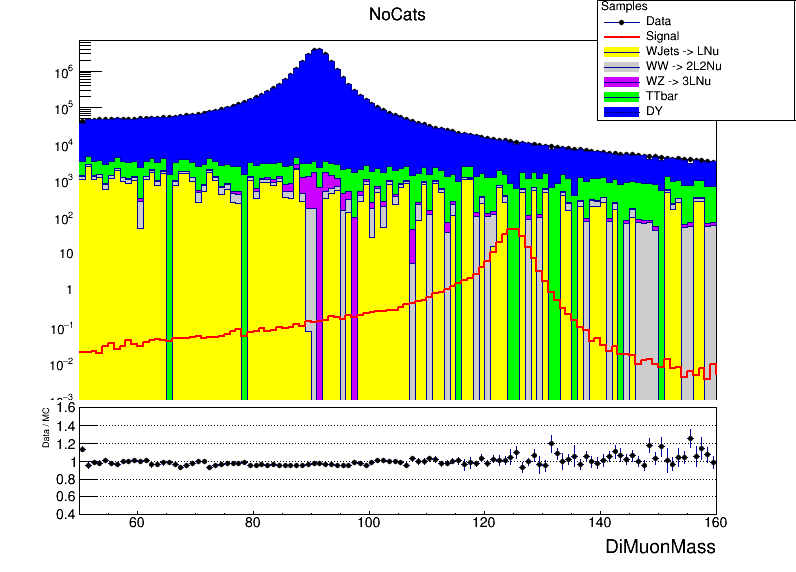
\includegraphics[width=0.9\linewidth]{figures/ch_higgs/distributions/baseline_rochester/distribution__NoCats__DiMuonMass__logY.png}\\
  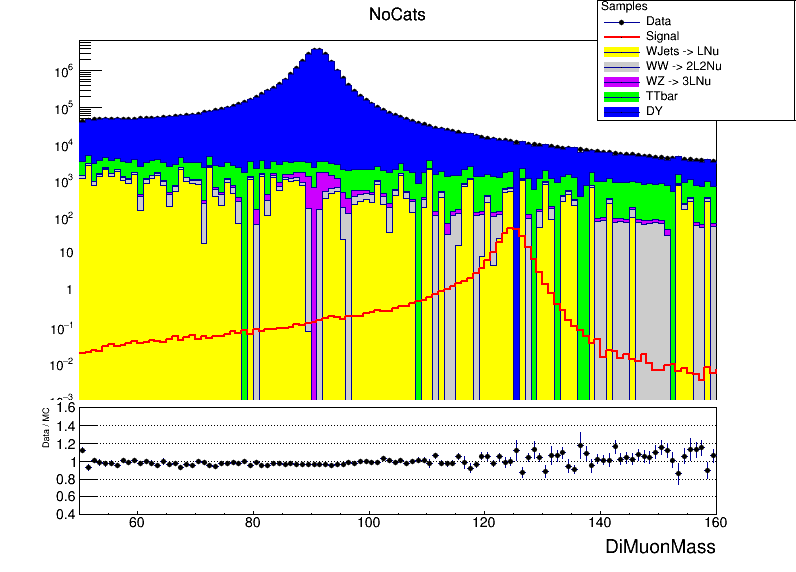
\includegraphics[width=0.9\linewidth]{figures/ch_higgs/distributions/baseline_kalman/distribution__NoCats__DiMuonMass__logY.png}
  \caption{Inclusive Dimuon Mass Distributions. Rochester (Left) and Kalman (Right) Corrections applied}
  \label{fig:higgs_selections_inclusivemass}
\end{figure}



% \subsection{Object validation}
% After applying all the selection cuts and scale factors, we validate the MC simulation
% on data events where the candidate muon pair has an invariant mass greater than 60~GeV.

% \begin{figure}[hbp]
%   \centering
%   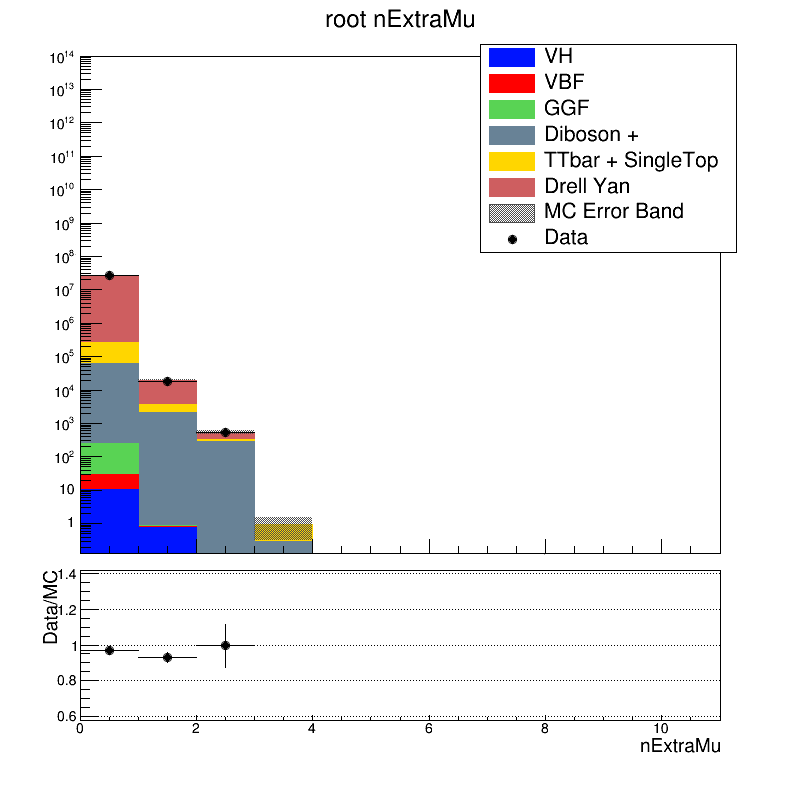
\includegraphics[width=0.32\linewidth]{figures/event_sel/nExtraMu_root.png}
%   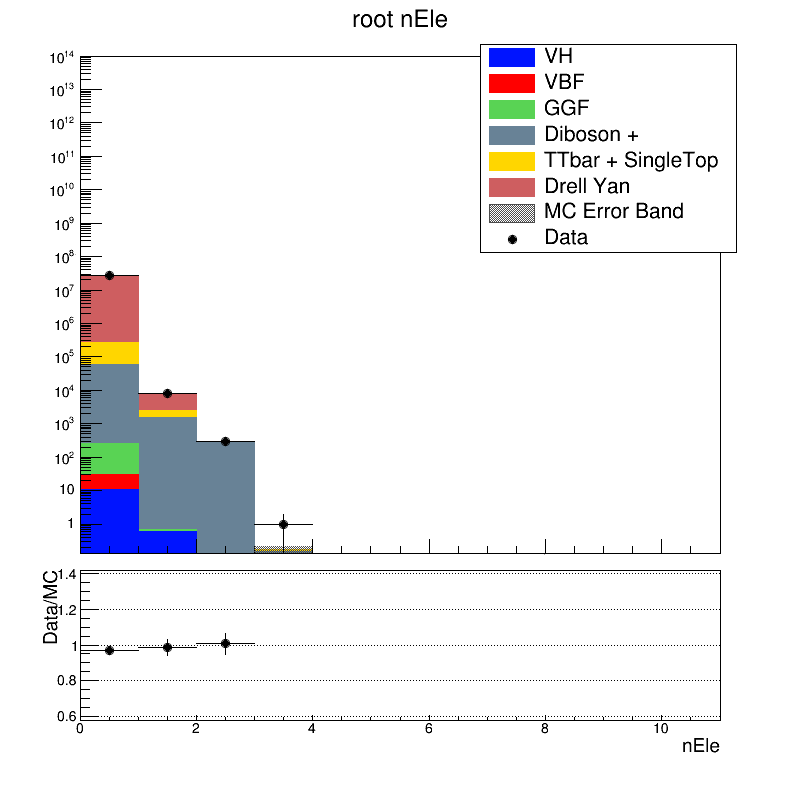
\includegraphics[width=0.32\linewidth]{figures/event_sel/nEle_root.png}
%   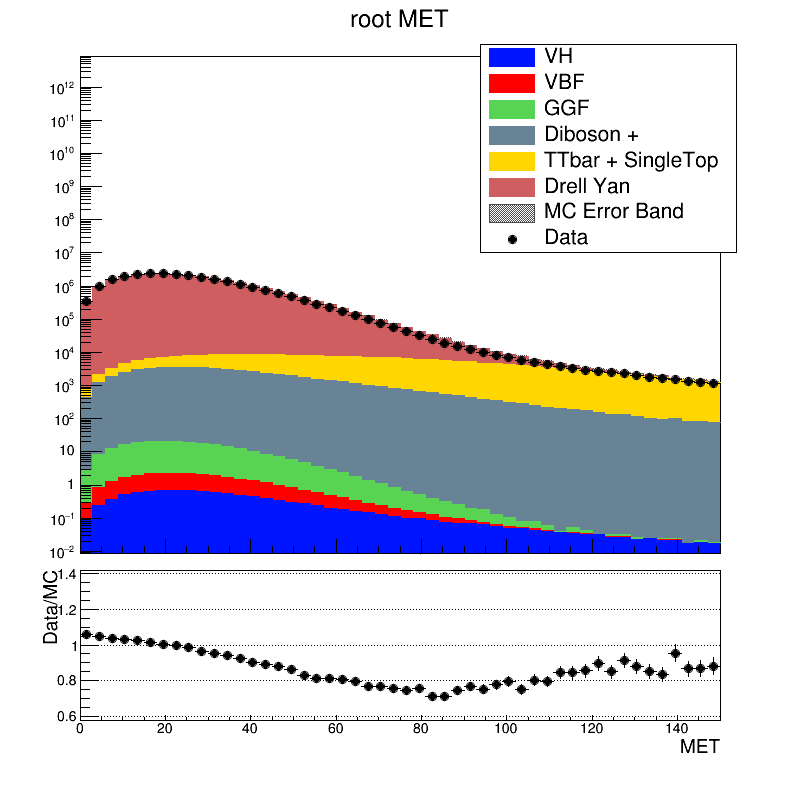
\includegraphics[width=0.32\linewidth]{figures/event_sel/MET_root.png}
%   \caption
%    {Validation of global event variables.}
%   \label{fig:valid_evt}
% \end{figure}

% \begin{figure}[hbp]
%   \centering
%   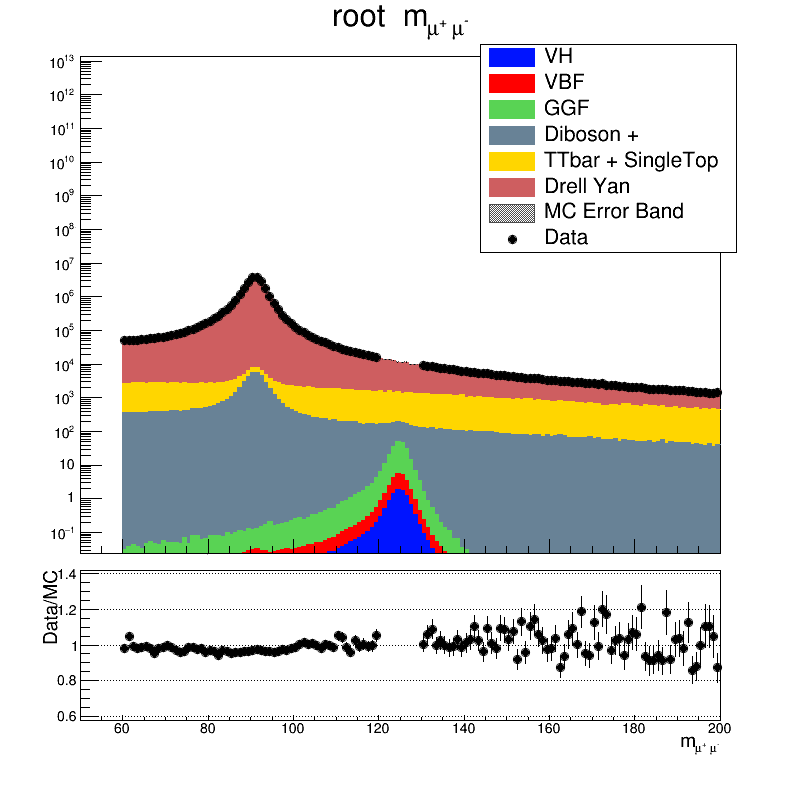
\includegraphics[width=0.32\linewidth]{figures/event_sel/dimu_mass_Roch_root.png}
%   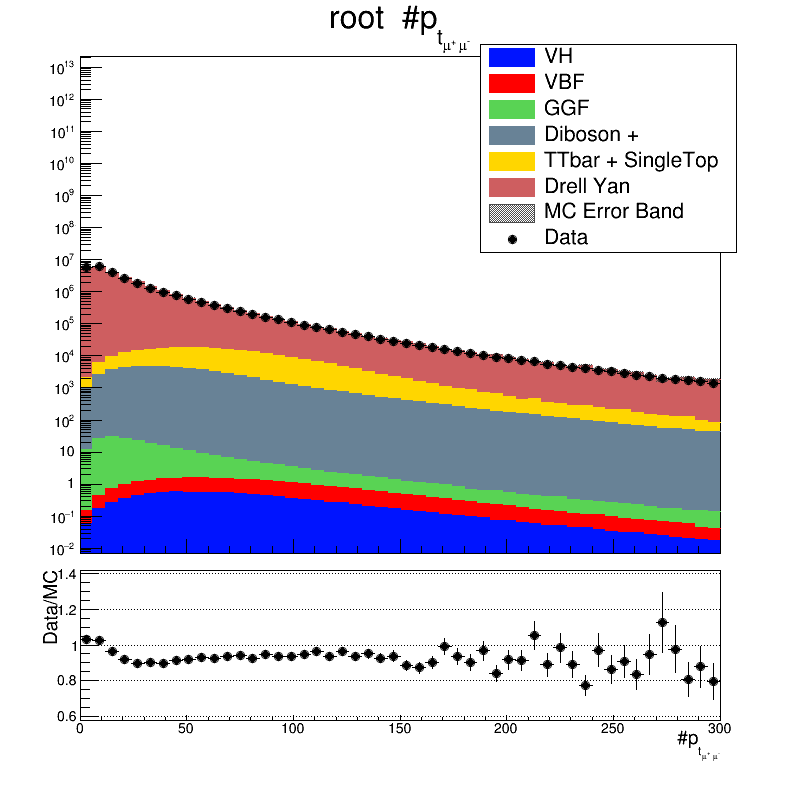
\includegraphics[width=0.32\linewidth]{figures/event_sel/dimu_pt_root.png}
%   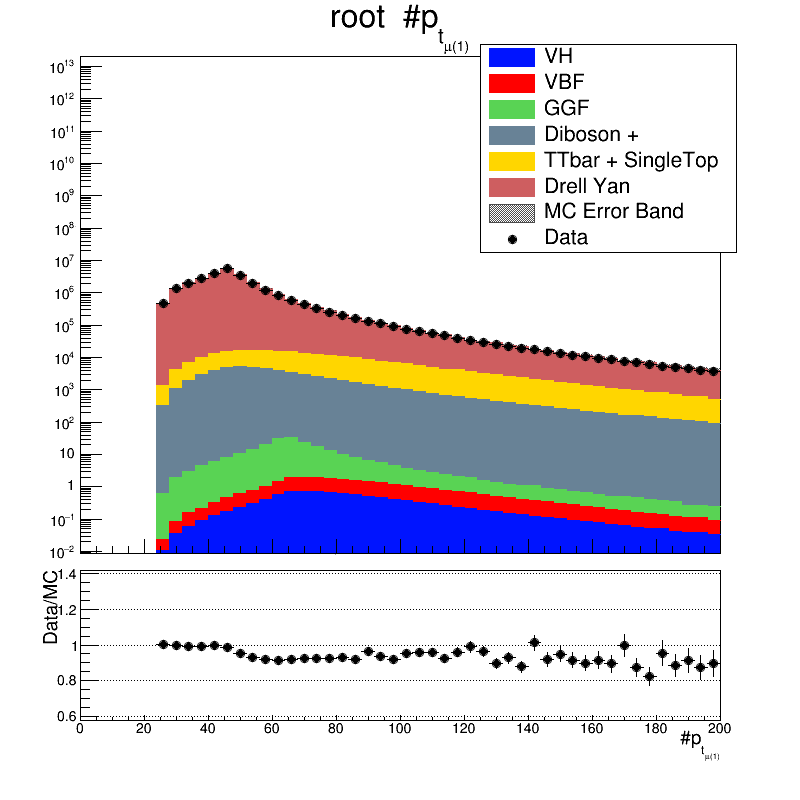
\includegraphics[width=0.32\linewidth]{figures/event_sel/mu1_pt_root.png}
%   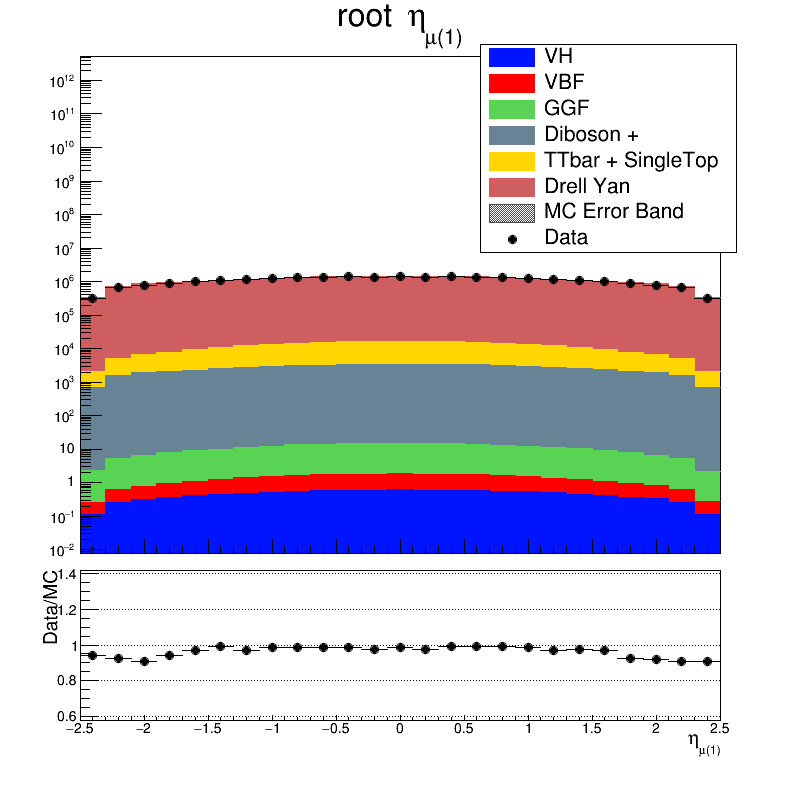
\includegraphics[width=0.32\linewidth]{figures/event_sel/mu1_eta_root.png}
%   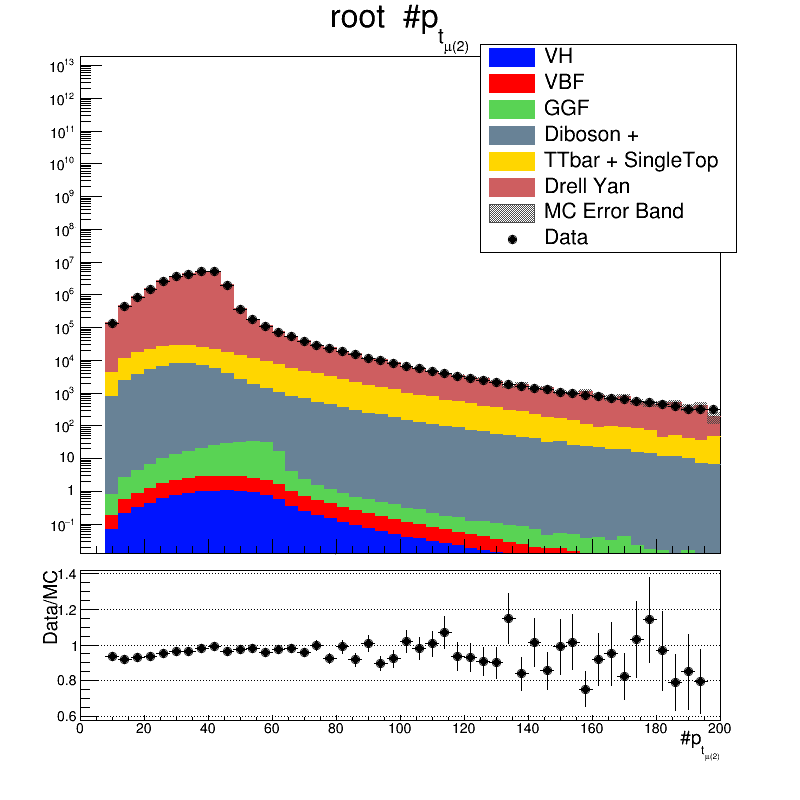
\includegraphics[width=0.32\linewidth]{figures/event_sel/mu2_pt_root.png}
%   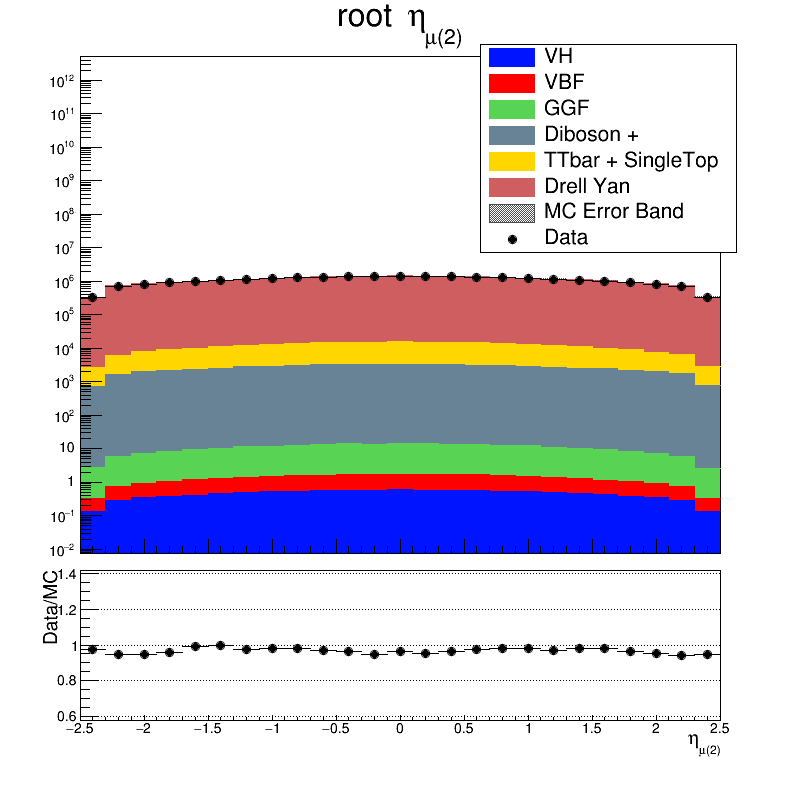
\includegraphics[width=0.32\linewidth]{figures/event_sel/mu2_eta_root.png}
%   \caption
%    {Validation of muon-related variables.}
%   \label{fig:valid_muons}
% \end{figure}

% \begin{figure}[hbp]
%   \centering
%   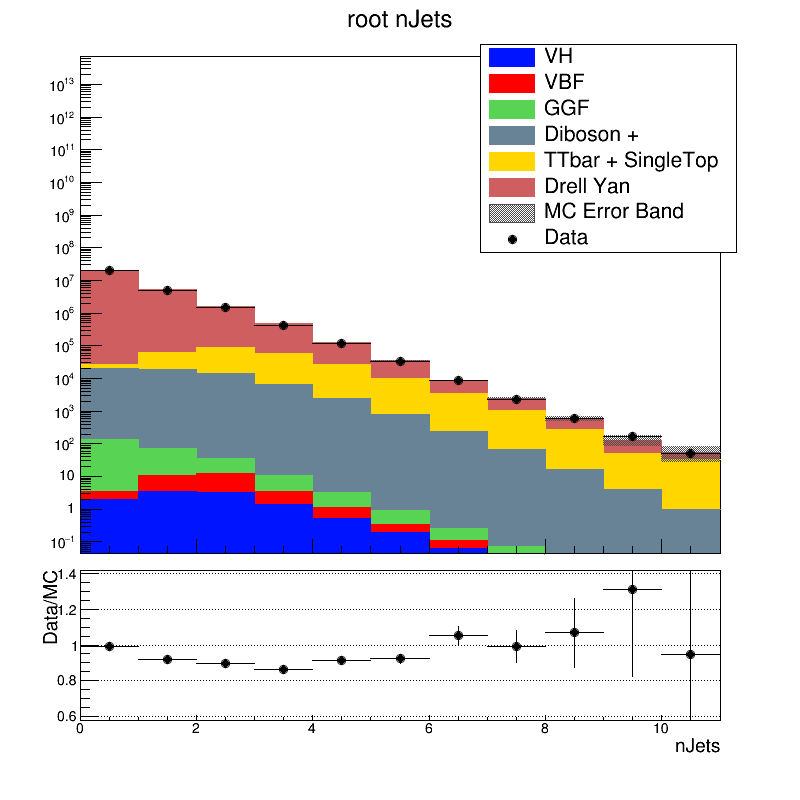
\includegraphics[width=0.32\linewidth]{figures/event_sel/nJets_root.png}
%   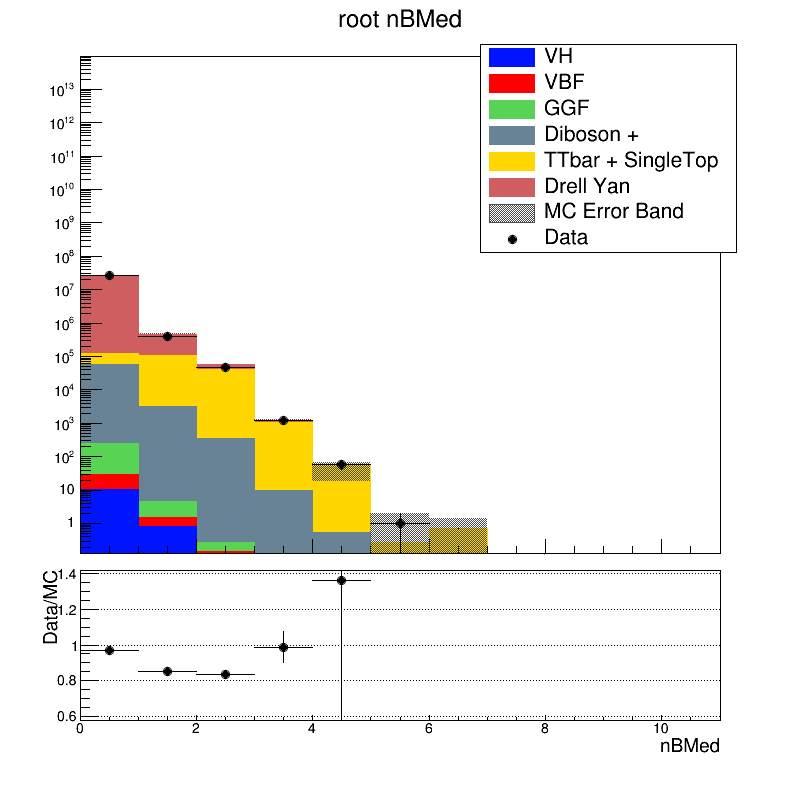
\includegraphics[width=0.32\linewidth]{figures/event_sel/nBMed_root.png}
%   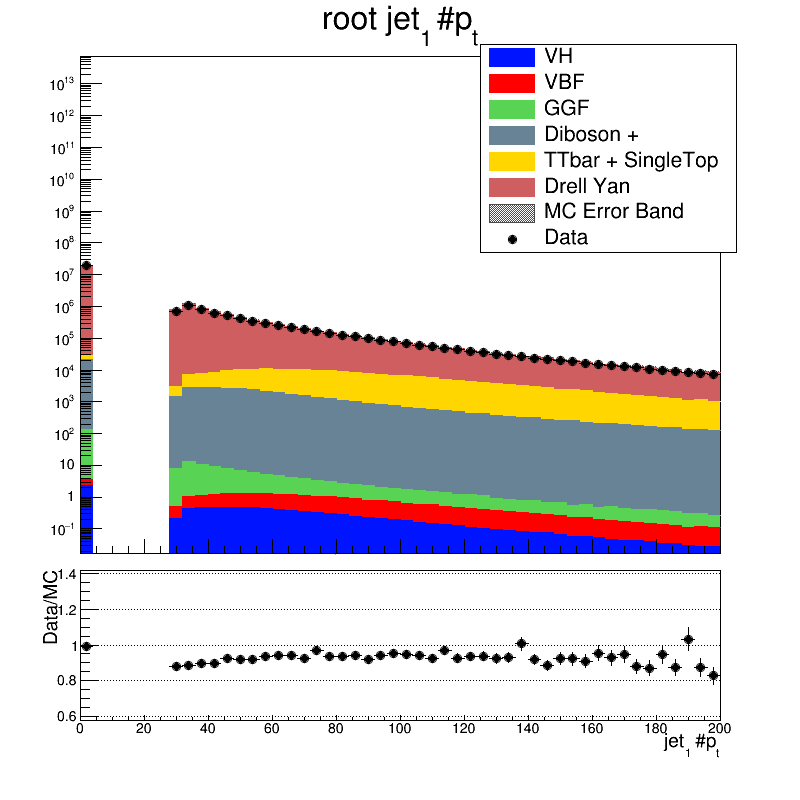
\includegraphics[width=0.32\linewidth]{figures/event_sel/jet1_pt_root.png}
%   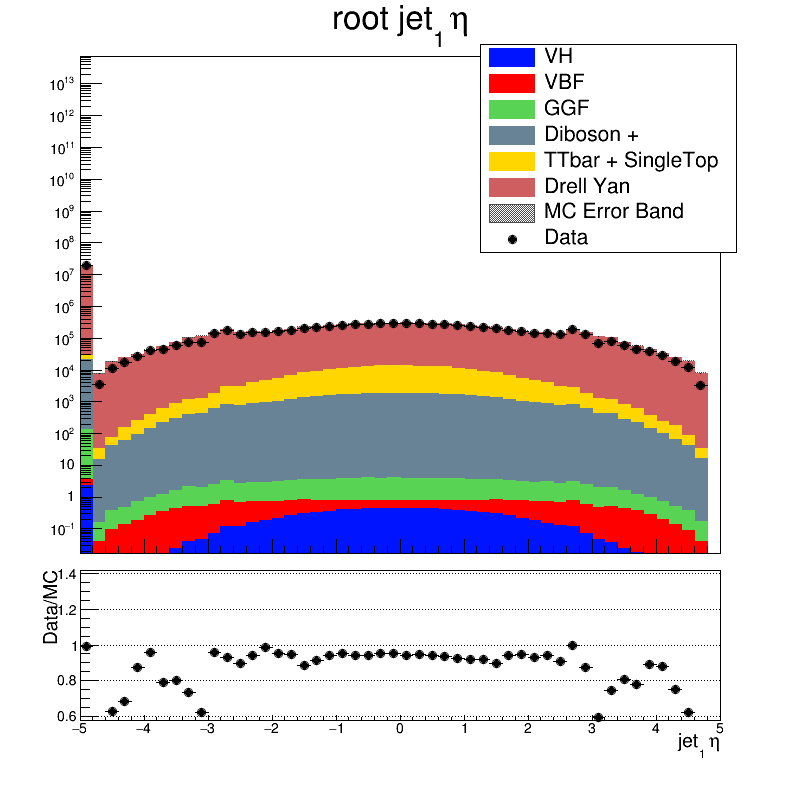
\includegraphics[width=0.32\linewidth]{figures/event_sel/jet1_eta_root.png}
%   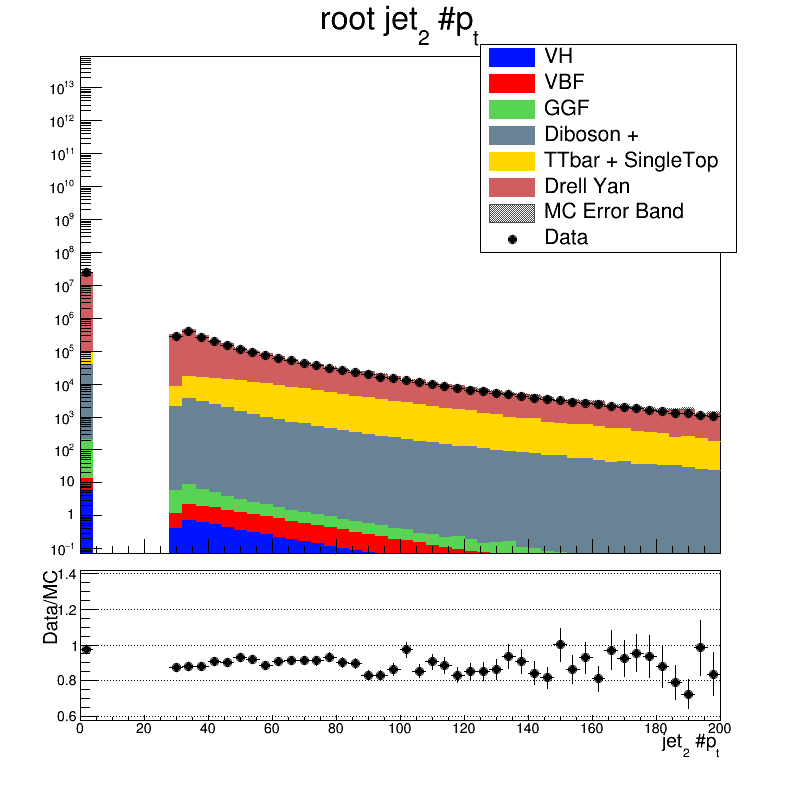
\includegraphics[width=0.32\linewidth]{figures/event_sel/jet2_pt_root.png}
%   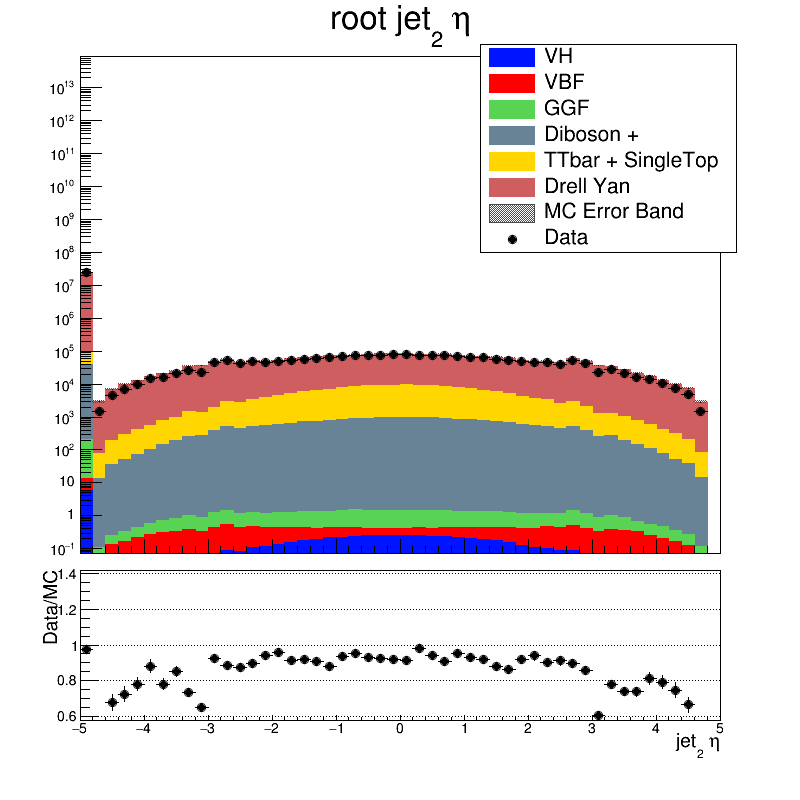
\includegraphics[width=0.32\linewidth]{figures/event_sel/jet2_eta_root.png}
%   \caption
%    {Validation of jet-related variables.}
%   \label{fig:valid_jets}
% \end{figure}




\section{Event Categorization}\label{section:higgs_categorization}
For the purpose of increasing the sensitivity of our analysis, the next step performed is the categorization of events into different subclasses. The basic idea is that we want to utilize the knowledge about two important characteristics of our search: the physics of interest, differences between the production processes, and the fact that our muon detectors intrinsically have better resolution for certain geometrical regions (barrel vs endcap). Using this information will allow us to substantially increase the significance of the Standard Model signal over the expected background.

\subsection{Baseline Categorization}
During the CMS Run I analysis campaign, the categorization procedure used was optimized to separate VBF like events from the rest by requiring the presence of at least 2 jets, pssing the Jet Selections, and going into the opposite ends of our detector and employing large Missing Transverse Energy (MET) selection. Moreover, the resolution of Muon System is significantly better in the Barrel region than in the Endcap, therefore we subdivide the space in $\eta$ variable by defining:
\begin{itemize}
  \item Barrel: $|\eta| < 0.8$
  \item Overlap: $|\eta| \ge 0.8$ \& $|\eta| < 1.6$
  \item Endcap: $|\eta| \ge 1.6$ \& $|\eta| < 2.1$
\end{itemize}
Furthermore, once we have a Higgs candidate pair, we tag each muon based on the region of the detector it was reconstructed in based on its $\eta$. The exact selections applied in the baseline categorization procedure follow:
\begin{itemize}
  \item $njets \ge 2$ \& $p_{t}^{j1} > 40$ GeV \& $p_{t}^{MET} < 40$ GeV - require at least 2 jets with thresholds on \pt of the leading jet and Missing Energy Transverse.
    \begin{itemize}
      \item VBFTight Category: $m_{jj} > 650$ GeV \& $|\Delta \eta| > 3.5$ - category targeting the Vector Boson Fusion production mechanism. The signature is the presence of 2 jets with a large invariant mass and going into opposite ends of CMS.
      \item GFTight Category: if not VBFTight \& $m_{jj} > 250$ GeV \& $p_{t}^{\mu\mu} > 50$ GeV. In this category, we target Gluon Fusion production together with what does not pass the VBF-like selections.
      \item GFLoose Category: here collect everything that does not pass the VBFTight and GFTight selections.
    \end{itemize}
  \item $njets \le 1$ - the biggest portion of the events will have only 1 or 0 jets total per event (that pass previously discussed selections).
    \begin{itemize}
      \item 01JetsTight Category - $p_t^{\mu\mu} \ge 25$ GeV. The only discriminating variable we are left with at this point is the \pt of the dimuon system that typically has higher values for the signal events.
        \begin{itemize}
          \item 01JetsTightBB: $\mu_{1,2}$ are Barrel
          \item 01JetsTightBE: $\mu_{1}$ is Barrel \& $\mu_2$ is Endcap
          \item 01JetsTightBO: $\mu_{1}$ is Barrel \& $\mu_2$ is Overlap
          \item 01JetsTightEE: $\mu_{1}$ is Endcap \& $\mu_2$ is Endcap
          \item 01JetsTightEO: $\mu_{1}$ is Endcap \& $\mu_2$ is Overlap
          \item 01JetsTightOO: $\mu_{1}$ is Overlap \& $\mu_2$ is Overlap
        \end{itemize}
      \item 01JetsLoose Category - Left over events fall into this category.
        \begin{itemize}
          \item 01JetsLooseBB: $\mu_{1,2}$ are Barrel
          \item 01JetsLooseBE: $\mu_{1}$ is Barrel \& $\mu_2$ is Endcap
          \item 01JetsLooseBO: $\mu_{1}$ is Barrel \& $\mu_2$ is Overlap
          \item 01JetsLooseEE: $\mu_{1}$ is Endcap \& $\mu_2$ is Endcap
          \item 01JetsLooseEO: $\mu_{1}$ is Endcap \& $\mu_2$ is Overlap
          \item 01JetsLooseOO: $\mu_{1}$ is Overlap \& $\mu_2$ is Overlap
        \end{itemize}
    \end{itemize}
\end{itemize}

Figures~\ref{fig:higgs_categorization_2jetsall}-~\ref{fig:higgs_categorization_01jetslooseeeeooo} show dimuon mass distributions for all of the terminal categories. For the final analysis, given that both Muon Corrections are producing similar results, we utilize Kalman Corrections. Data in all of the categories is modelled well by the included backgrounds.
\begin{figure}[H]
  \centering
  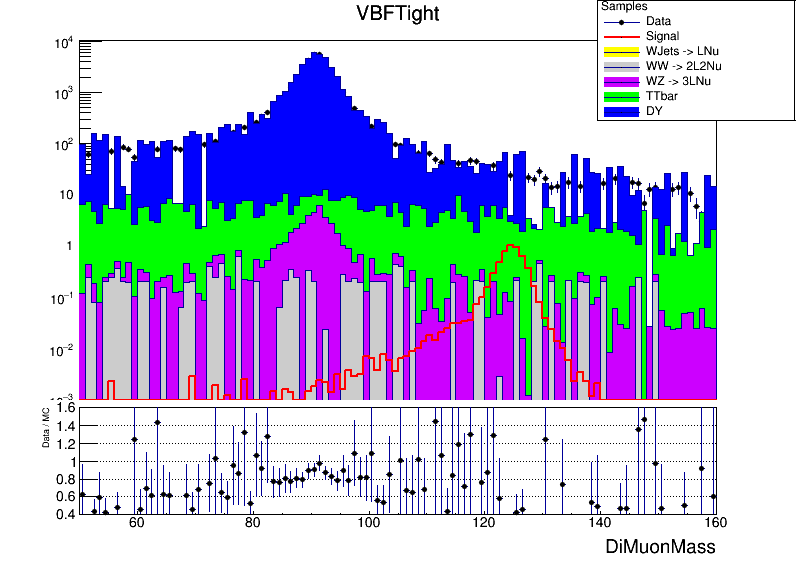
\includegraphics[width=0.65\linewidth]{figures/ch_higgs/distributions/baseline_kalman/distribution__VBFTight__DiMuonMass__logY.png}\\
  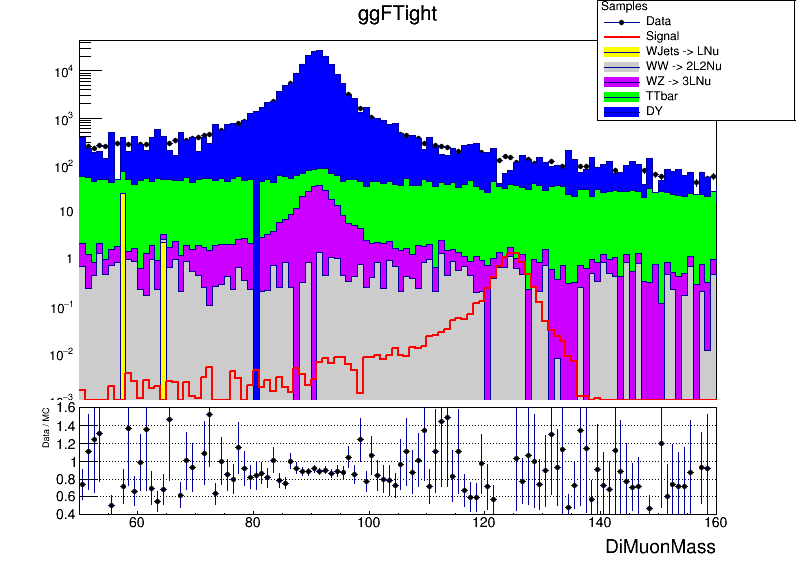
\includegraphics[width=0.65\linewidth]{figures/ch_higgs/distributions/baseline_kalman/distribution__ggFTight__DiMuonMass__logY.png}\\
  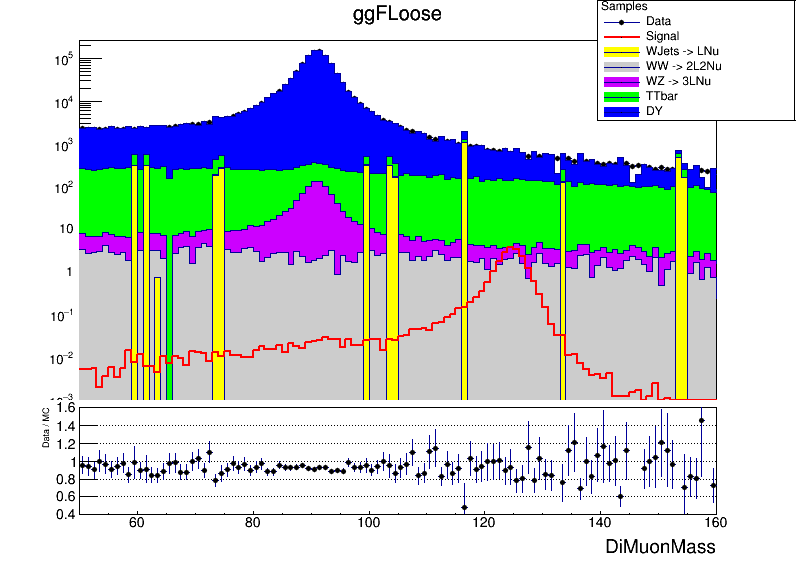
\includegraphics[width=0.65\linewidth]{figures/ch_higgs/distributions/baseline_kalman/distribution__ggFLoose__DiMuonMass__logY.png}
  \caption{Mass Distributions VBFTight (Top), GFTight (Middle) and GFLoose (Bottom) Categories.}
  \label{fig:higgs_categorization_2jetsall}
\end{figure}
\begin{figure}[H]
  \centering
  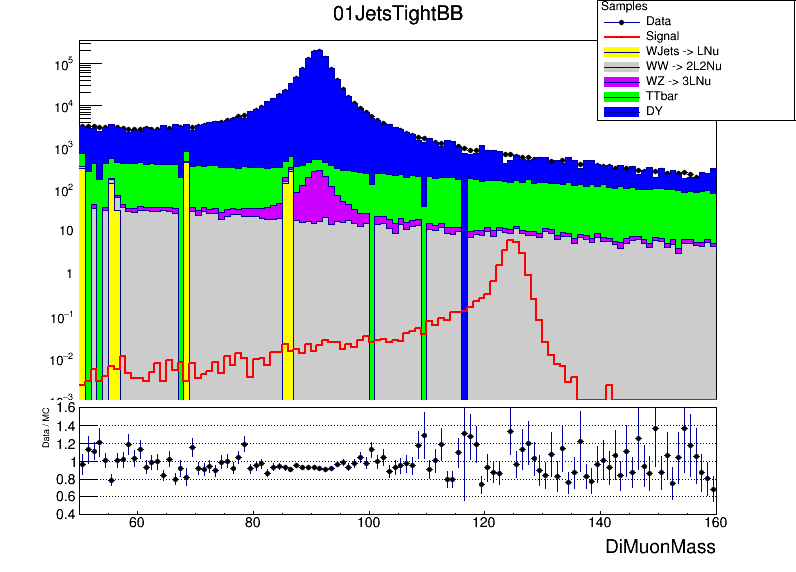
\includegraphics[width=0.65\linewidth]{figures/ch_higgs/distributions/baseline_kalman/distribution__01JetsTightBB__DiMuonMass__logY.png}\\
  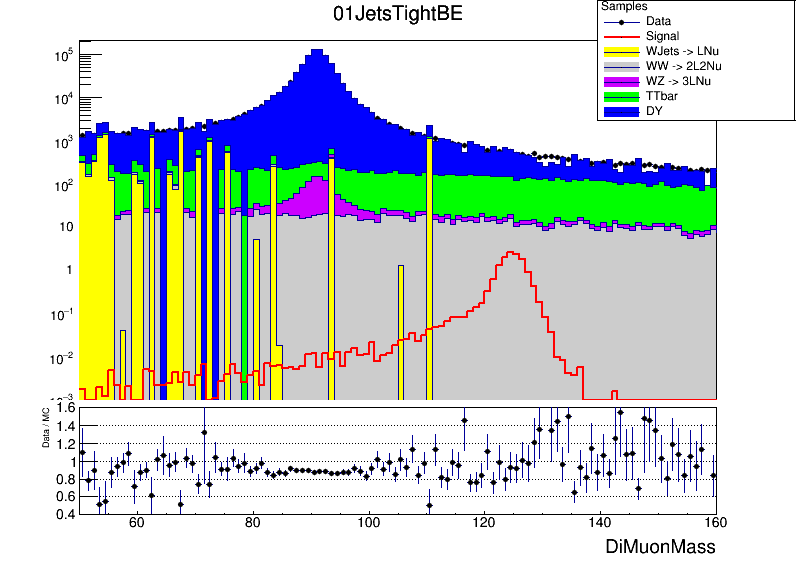
\includegraphics[width=0.65\linewidth]{figures/ch_higgs/distributions/baseline_kalman/distribution__01JetsTightBE__DiMuonMass__logY.png}\\
  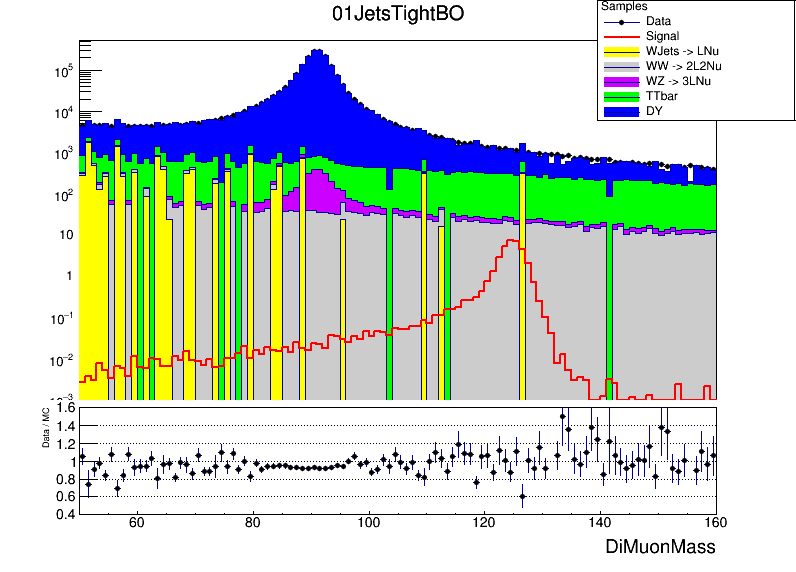
\includegraphics[width=0.65\linewidth]{figures/ch_higgs/distributions/baseline_kalman/distribution__01JetsTightBO__DiMuonMass__logY.png}
  \caption{Mass Distributions 01JetsTightBB (Top), 01JetsTightBE (Middle) and 01JetsTightBO (Bottom) Categories.}
  \label{fig:higgs_categorization_01jetstightbbbebo}
\end{figure}
\begin{figure}[H]
  \centering
  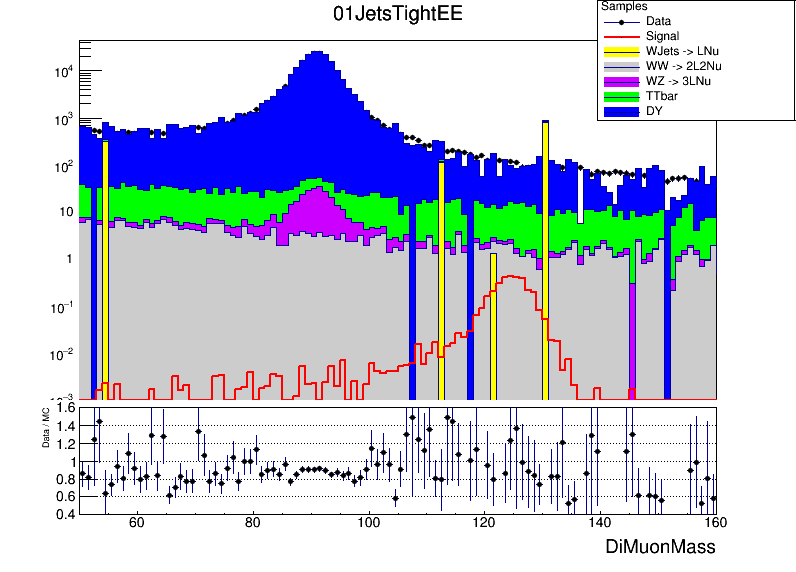
\includegraphics[width=0.65\linewidth]{figures/ch_higgs/distributions/baseline_kalman/distribution__01JetsTightEE__DiMuonMass__logY.png}\\
  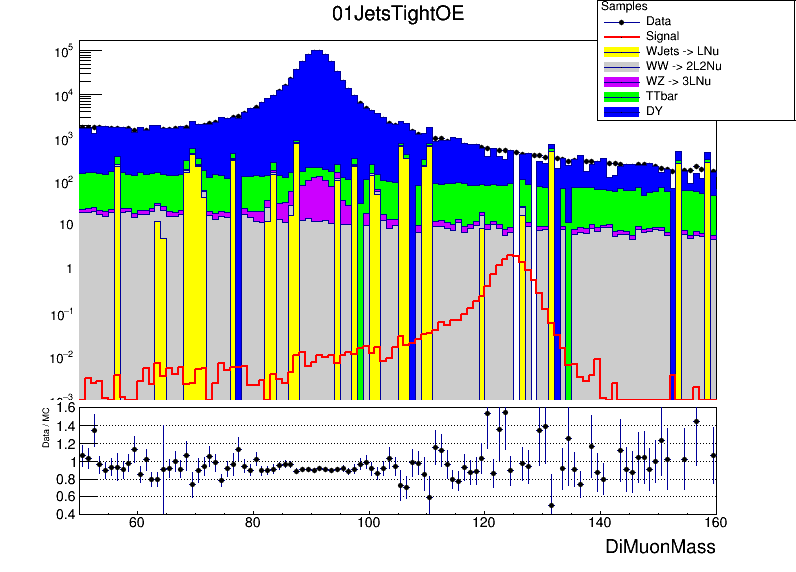
\includegraphics[width=0.65\linewidth]{figures/ch_higgs/distributions/baseline_kalman/distribution__01JetsTightOE__DiMuonMass__logY.png}\\
  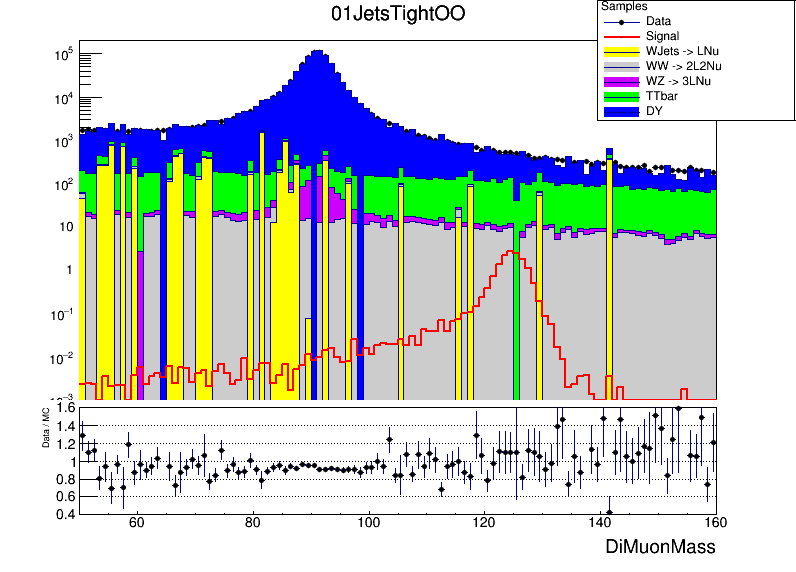
\includegraphics[width=0.65\linewidth]{figures/ch_higgs/distributions/baseline_kalman/distribution__01JetsTightOO__DiMuonMass__logY.png}
  \caption{Mass Distributions 01JetsTightEE (Top), 01JetsTightOE (Middle) and 01JetsTightOO (Bottom) Categories.}
  \label{fig:higgs_categorization_01jetstighteeeooo}
\end{figure}
\begin{figure}[H]
  \centering
  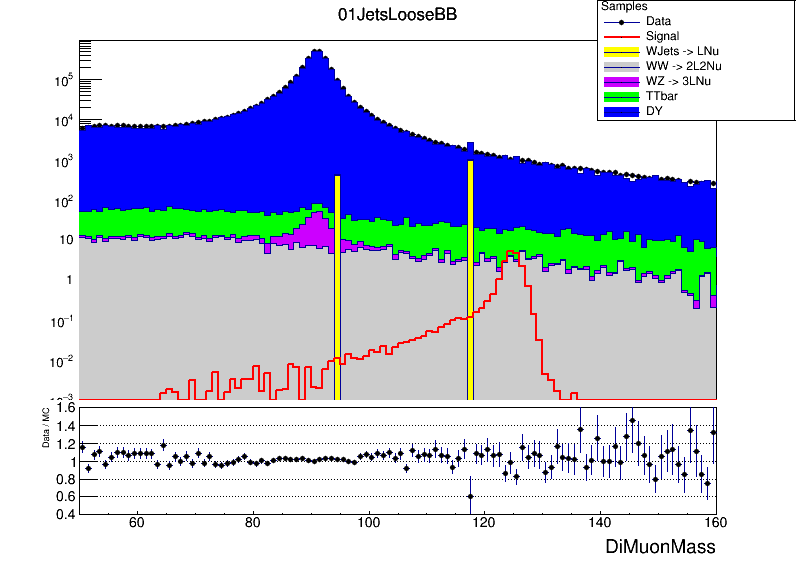
\includegraphics[width=0.65\linewidth]{figures/ch_higgs/distributions/baseline_kalman/distribution__01JetsLooseBB__DiMuonMass__logY.png}\\
  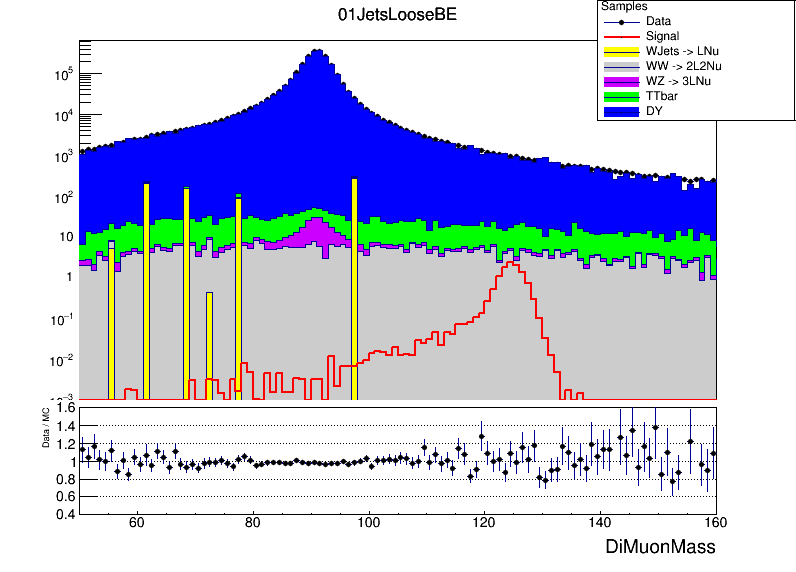
\includegraphics[width=0.65\linewidth]{figures/ch_higgs/distributions/baseline_kalman/distribution__01JetsLooseBE__DiMuonMass__logY.png}\\
  \includegraphics[width=0.65\linewidth]{figures/ch_higgs/distributions/baseline_kalman/distribution__01JetsLooseBO__DiMuonMass__logY.png}
  \caption{Mass Distributions 01JetsLooseBB (Top), 01JetsLooseBE (Middle) and 01JetsLooseBO (Bottom) Categories.}
  \label{fig:higgs_categorization_01jetsloosebbbebo}
\end{figure}
\begin{figure}[H]
  \centering
  \includegraphics[width=0.65\linewidth]{figures/ch_higgs/distributions/baseline_kalman/distribution__01JetsLooseEE__DiMuonMass__logY.png}\\
  \includegraphics[width=0.65\linewidth]{figures/ch_higgs/distributions/baseline_kalman/distribution__01JetsLooseOE__DiMuonMass__logY.png}\\
  \includegraphics[width=0.65\linewidth]{figures/ch_higgs/distributions/baseline_kalman/distribution__01JetsLooseOO__DiMuonMass__logY.png}
  \caption{Mass Distributions 01JetsLooseEE (Top), 01JetsLooseOE (Middle) and 01JetsLooseOO (Bottom) Categories.}
  \label{fig:higgs_categorization_01jetslooseeeeooo}
\end{figure}

\subsection{Greedy Categorization} \label{bdt_training}
Another approach taken was to optimize the manually constructed categorization tree, discussed in the previous section, in a more systematic way by, first, training and applying a Boosted Decision Tree (BDT) for the purpose of signal to background discrimination and, then, using the BDT ouput as a new input feature for optimizing the categorization tree using a greedy optimization procedure.

In the first step, the BDT for the signal to background discrimination has been trained using both signal and background Monte Carlo samples. The BDT implementation from the {\sc ROOT}~\cite{ROOT} framework has been successfully used. Given that background samples are not utilized for the statistical analysis (we use data-driven background treatment discussed further), we employ all of the available MC background events for the purpose of training, cross-validation and testing. However, in terms of the Higgs signal, the even-numbered events are used for the categorization optimization. The rest is reserved for the statistical analysis. The following kinematic variables are used as input features for the BDT:
\begin{itemize}
  \item The $p_t^{\mu\mu}$ of the dimuon system
  \item The $\eta_{\mu\mu}$ of the dimuon system.
  \item The $|\Delta \eta|$ between the muons from the Higgs candidate.
  \item The $|\Delta \phi|$ between the muons from the Higgs candidate.
  \item The $\eta_{jj}$ of the dijet system. 2 highest $p_t$ jets are used.
  \item The $m_{jj}$ of the dijet system. 2 highest $p_t$ jets are used.
  \item The $|\Delta \eta|$ between the 2 highest $p_t$ jets.
  \item The number of Central jets with $|\eta| < 2.4$
  \item The number of Forward jets with $|\eta| > 2.4$
  \item The number of b-tagged jets - jets passing the CSVv2 medium b-tag working point
  \item The \MET
\end{itemize}
As it follows from the above list, there is no dependence on the Higgs candidate mass among the features directly or indirectly. In other words, given the above features, one can not deduce the mass value of the dimuon system. Given that we are performing a search and all of the mass points available will be passed through the same BDT after determining the weights, mass independence is an importan criteria of our discrimination technique.

After the training and cross-validation to tune the hyper parameters of the Decision Tree itself, we run over the test dataset and figure~\ref{fig:higgs_categorization_bdtoutputroc} shows the BDT ouput distributions for both training and testing subsets, which are in a very good agreement. It is a clear sign that we did not overtrain. Furthermore, the ROC curve from figure~\ref{fig:higgs_categorization_bdtoutputroc}, which is an indicator of the efficiency of our selection and rejection at the same time, shows a definite deviation from the diagonal (no discrimination), however even with 100\% inefficiency on background rejection, we still fall short of 100\% of signal rejection. Finally, given that we are not choosing a turning point and not doing a pure binary classficiation, we preserve the BDT score for the next stage.
\begin{figure}[hbp]
  \centering
  \includegraphics[width=0.75\linewidth]{figures/bdt_training/BDT_out_ge0j_all.pdf}\\
  \includegraphics[width=0.75\linewidth]{figures/bdt_training/BDT_ROC_ge0j_all.pdf}
  \caption{BDT score distribution (Top) and Receiver Operating Curve, ROC, (Bottom) - a kind of True Negative/Positive selection efficiency indicator.}
  \label{fig:higgs_categorization_bdtoutputroc}
\end{figure}

The next step of the Greedy Categorization procedure is to optimize the categorization tree selections and perform the actual splitting of events into different subsets. For that purpose, a simple decision tree is used with a custom metric, signal significance, and with the following 2 features:
\begin{itemize}
  \item max($\eta_{\mu_1}$, $\eta_{\mu_2}$) - max $\eta among the muons from the Higgs Candidate pair$
  \item Discriminting BDT score
\end{itemize}
Again, only part of the signal has been used for the training, whereas all of the background events have been passed through the custom decision tree.

Before moving forward with the actual algorithm, we have to provide a few definitions. First of all, we have to acknowledge, that the objects we are going to work with are the dimuon mass histogrammes as in figure~\ref{fig:higgs_categorization_massc0}. For a given mass distribution, we define a Signal Significance ($S_{node}$) according to the equation~\ref{eq:higgs_categorization_significance}. $N^{S}_{c,i}$ and $N^{B}_{c,i}$ are the yields (number of entries) for that particular histogram and for that particular bin. Note that we treat all the bins in the distribution separately and only use those that fall in the [120 GeV, 130 GeV] mass range. Futhermore, the metric, based on which we are going to optimize the splitting, is provided in equation~\ref{eq:higgs_categorization_gain}. Roughly speaking, we use the split that gives us the maximum gain across all the splits that have been tried.
\begin{figure}[hbp]
  \centering
  \includegraphics[width=0.9\linewidth]{figures/ch_higgs/distributions/bdt_uf/distribution__c0__DiMuonMass__logY.png}
  \caption{Mass Distribution for Category ''c0'' - lowest Discriminating BDT score category}
  \label{fig:higgs_categorization_massc0}
\end{figure}
\begin{equation}
  {S^2_c} = \sum_{c,i}N^{S2}_{c,i}/N^{B}_{c,i}
  \label{eq:higgs_categorization_significance}
\end{equation}
\begin{equation}
  {G} = {S^2_{left}} + {S^2_{right}} - {S^2_{node}}
  \label{eq:higgs_categorization_gain}
\end{equation}

After providing all of the important definitions to work with, the actual procedure for the tree splits optimization can be summarized as follows:
\begin{itemize}
  \item Stage 1. Start out with the inclusive set of all events - a node.
  \item Stage 2. Greedily scan through the features and select the split:
    \begin{itemize}
      \item Scan through all of the possible values of max($\eta_{\mu_1}$, $\eta_{\mu_2}$) as split's candidates. Save the split that produces maximum gain.
      \item Scan through all of the possible values of the BDT score. Again, save the split that maximizes the gain for the second feature.
      \item Select the split which maximizes the gain: max(G$_\eta$, G$_{score}$)
    \end{itemize}
  \item Stage n. Repeat Stage 2 recursively for each of the new nodes until the tree reaches the limit on the number of categories or runs out of splitting conditions.
\end{itemize}
The procedure just described is an example of a greedy algorithm, because we do not perform full parameters' phase space optimization as it is computationally infeasible. We greedily optimize the metric of interest step by step iterating over all of the available features.

The outcome of this technique is 13 new categories with the categorization tree shown in figure~\ref{fig:higgs_categorization_bdtcategories}. Integer labels are assigned based on the trained sensitivity of a particular subset, going from the category with the lowest sensitivity, ''c0'', to the one with the highest, ''c12''.
\begin{figure}[hbp]
  \centering
  \includegraphics[width=1.0\linewidth]{figures/bdt_cats/final_categories.png}
  \caption
   {Greedy Categorization Tree.}
  \label{fig:higgs_categorization_bdtcategories}
\end{figure}

\begin{figure}[H]
  \centering
  \includegraphics[width=0.65\linewidth]{figures/ch_higgs/distributions/bdt_uf/distribution__c1__DiMuonMass__logY.png}\\
  \includegraphics[width=0.65\linewidth]{figures/ch_higgs/distributions/bdt_uf/distribution__c2__DiMuonMass__logY.png}\\
  \includegraphics[width=0.65\linewidth]{figures/ch_higgs/distributions/bdt_uf/distribution__c3__DiMuonMass__logY.png}
  \caption{Mass Distributions for c1-c3 subsets from the Greedy Categorization}
  \label{fig:higgs_categorization_greedyc1c3}
\end{figure}
\begin{figure}[H]
  \centering
  \includegraphics[width=0.65\linewidth]{figures/ch_higgs/distributions/bdt_uf/distribution__c4__DiMuonMass__logY.png}\\
  \includegraphics[width=0.65\linewidth]{figures/ch_higgs/distributions/bdt_uf/distribution__c5__DiMuonMass__logY.png}\\
  \includegraphics[width=0.65\linewidth]{figures/ch_higgs/distributions/bdt_uf/distribution__c6__DiMuonMass__logY.png}
  \caption{Msas Distributions for c4-c6 subsets from the Greedy Categorization}
  \label{fig:higgs_categorization_greedyc4c6}
\end{figure}
\begin{figure}[H]
  \centering
  \includegraphics[width=0.65\linewidth]{figures/ch_higgs/distributions/bdt_uf/distribution__c7__DiMuonMass__logY.png}\\
  \includegraphics[width=0.65\linewidth]{figures/ch_higgs/distributions/bdt_uf/distribution__c8__DiMuonMass__logY.png}\\
  \includegraphics[width=0.65\linewidth]{figures/ch_higgs/distributions/bdt_uf/distribution__c9__DiMuonMass__logY.png}
  \caption{Mass Distributions for c7-c9 subsets from the Greedy Categorization}
  \label{fig:higgs_categorization_greedyc7c9}
\end{figure}
\begin{figure}[H]
  \centering
  \includegraphics[width=0.65\linewidth]{figures/ch_higgs/distributions/bdt_uf/distribution__c10__DiMuonMass__logY.png}\\
  \includegraphics[width=0.65\linewidth]{figures/ch_higgs/distributions/bdt_uf/distribution__c11__DiMuonMass__logY.png}\\
  \includegraphics[width=0.65\linewidth]{figures/ch_higgs/distributions/bdt_uf/distribution__c12__DiMuonMass__logY.png}
  \caption{Mass Distributions for c10-c12 subsets fomr the Greedy Categorization}
  \label{fig:higgs_categorization_greedyc10c12}
\end{figure}

Figures~\ref{fig:higgs_categorization_greedyc1c3}-~\ref{fig:higgs_categorization_greedyc10c12} summarize the resulting dimuon mass distributions. The modeling of the dimuon mass agrees well between data and simulations. Furthermore, figures~\ref{fig:higgs_categorization_bdtinput1_inclusive},~\ref{fig:higgs_categorization_bdtinput2_inclusive} provide the comparison of the data with Monte Carlo for the kinematic variables, input features, that are used for the signal discrimination. Figures~\ref{fig:higgs_categorization_bdtinput1_c12},~\ref{fig:higgs_categorization_bdtinput2_c12} show the same features but compared for the most sensitive category. Overall, good agreement between data and simulations is observed, especially for the dimuon mass distribution. Finally, Table~\ref{tab:higgs_categorization_yields} provides a summary on the statistical properties of dimuon mass shapes provided in figures~\ref{fig:higgs_categorization_greedyc1c3}-~\ref{fig:higgs_categorization_greedyc10c12}. One of the important characteristics of our search, although not obvious, is the signal width, provided in terms of Full Width at Half Maximum (FWHM). It is an important feature because the smaller the width is, the more pronounced the signal is, the less influence the shape of the function, used for the background estimation, will have on our Standard Model Higgs signal.
\begin{table}[htb]
  \caption{Comparison of Signal and Background Yields for greedily optimized categories.}
  \label{tab:higgs_categorization_yields}
  \begin{center}
    \begin{tabular}{|c|c|c|c|c|c|}
      \hline
      Category  & Signal FWHM & $N^{S}$ & $N^{B}$ & $\mathrm{N^S / \sqrt{N^B}}$ \\
      \hline
      c0 & 4.4 & 13.4826 & 14187.6 & 0.113193\\
      c1 & 5.8 & 3.52888 & 970.875 & 0.113255\\
      c2 & 5.8 & 14.2112 & 8248.64 & 0.156473\\
      c3 & 6.0 & 3.82012 & 779.594 & 0.136818\\
      c4 & 3.0 & 9.92363 & 1609.08 & 0.24739\\
      c5 & 2.8 & 8.5825  & 1028.08 & 0.267671\\
      c6 & 4.0 & 14.1224 & 2371.09 & 0.290025\\
      c7 & 4.2 & 26.3575 & 6904.16 & 0.317211\\
      c8 & 3.6 & 35.6493 & 11187.4 & 0.337043\\
      c9 & 4.0 & 6.12457 & 451.281 & 0.288305\\
      c10 & 4.0 & 13.9349 & 1667.59 & 0.34124\\
      c11 & 3.0 & 9.59255 & 765.226 & 0.346768\\
      c12 & 4.0 & 9.58541 & 420.983 & 0.467173\\
      \hline
    \end{tabular}
  \end{center}
\end{table}
\begin{figure}[hbp]
  \centering
  \includegraphics[width=0.49\linewidth]{figures/bdt_cats/dimu_eta_root.png}
  \includegraphics[width=0.49\linewidth]{figures/bdt_cats/dimu_abs_dEta_root.png}\\
  \includegraphics[width=0.49\linewidth]{figures/bdt_cats/dimu_abs_dPhi_root.png}
  \includegraphics[width=0.49\linewidth]{figures/bdt_cats/nJetsCent_root.png}
  \caption{Data/MC agreement for the BDT input variables before categorization.}
  \label{fig:higgs_categorization_bdtinput1_inclusive}
\end{figure}

\begin{figure}[hbp]
  \centering
  \includegraphics[width=0.49\linewidth]{figures/bdt_cats/dijet1_mass_root.png}
  \includegraphics[width=0.49\linewidth]{figures/bdt_cats/dijet1_abs_dEta_root.png}\\
  \includegraphics[width=0.49\linewidth]{figures/bdt_cats/dijet2_mass_root.png}
  \includegraphics[width=0.49\linewidth]{figures/bdt_cats/dijet2_abs_dEta_root.png}
  \caption{Data/MC agreement for the BDT input variables before categorization.}
  \label{fig:higgs_categorization_bdtinput2_inclusive}
\end{figure}

\begin{figure}[hbp]
  \centering
  \includegraphics[width=0.49\linewidth]{figures/bdt_cats/dimu_eta_c12.png}
  \includegraphics[width=0.49\linewidth]{figures/bdt_cats/dimu_abs_dEta_c12.png}\\
  \includegraphics[width=0.49\linewidth]{figures/bdt_cats/dimu_abs_dPhi_c12.png}
  \includegraphics[width=0.49\linewidth]{figures/bdt_cats/nJetsCent_c12.png}
  \caption{Data/MC agreement for the BDT input varaibles for the most sensitive category.}
  \label{fig:higgs_categorization_bdtinput1_c12}
\end{figure}

\begin{figure}[hbp]
  \centering
  \includegraphics[width=0.49\linewidth]{figures/bdt_cats/dijet1_mass_c12.png}
  \includegraphics[width=0.49\linewidth]{figures/bdt_cats/dijet1_abs_dEta_c12.png}\\
  \includegraphics[width=0.49\linewidth]{figures/bdt_cats/dijet2_mass_c12.png}
  \includegraphics[width=0.49\linewidth]{figures/bdt_cats/dijet2_abs_dEta_c12.png}
  \caption{Data/MC agreement for the BDT input variables for the most sensitive category.}
  \label{fig:higgs_categorization_bdtinput2_c12}
\end{figure}

% \begin{figure}
%   \includegraphics[width=1.0\linewidth]{figures/bdt_training/BDT_in_ge0j_all.pdf}
%   \includegraphics[width=1.0\linewidth]{figures/bdt_training/BDT_in_ge0j_sep.pdf}
%   \caption{Some BDT input variables for events with $\ge 0$ jets.
%            In the top plots, signal is in blue and background in red.
%            In the bottom plots, the gluon-fusion signal is dark blue, VBF is red, and VH is green,
%            while Drell--Yan and diboson backgrounds are pink, and \ttbar and single top are light blue.}
%   \label{fig:BDT_in_ge0j}
% \end{figure}

% \begin{figure}
%   \includegraphics[width=1.0\linewidth]{figures/bdt_training/BDT_in_le1j_all_A.pdf}
%   \includegraphics[width=1.0\linewidth]{figures/bdt_training/BDT_in_le1j_sep_A.pdf}
%   \caption{Some BDT input variables for events with $\le 1$ jets.
%            In the top plots, signal is in blue and background in red.
%            In the bottom plots, the gluon-fusion signal is dark blue, VBF is red, and VH is green,
%            while Drell--Yan and diboson backgrounds are pink, and \ttbar and single top are light blue.}
%   \label{fig:BDT_in_le1j_A}
% \end{figure}

% \begin{figure}
%   \includegraphics[width=1.0\linewidth]{figures/bdt_training/BDT_in_le1j_all_B.pdf}
%   \includegraphics[width=1.0\linewidth]{figures/bdt_training/BDT_in_le1j_sep_B.pdf}
%   \caption{Some BDT input variables for events with $\le 1$ jets.
%            In the top plots, signal is in blue and background in red.
%            In the bottom plots, the gluon-fusion signal is dark blue, VBF is red, and VH is green,
%            while Drell--Yan and diboson backgrounds are pink, and \ttbar and single top are light blue.}
%   \label{fig:BDT_in_le1j_B}
% \end{figure}

% \begin{figure}
%   \includegraphics[width=1.0\linewidth]{figures/bdt_training/BDT_in_eq2j_sep_B.pdf}
%   \caption{Some BDT input variables for events with $= 2$ jets.
%            The gluon-fusion signal is dark blue, VBF is red, and VH is green,
%            while Drell--Yan and diboson backgrounds are pink, and \ttbar and single top are light blue.}
%   \label{fig:BDT_in_eq2j_B}
% \end{figure}

% \begin{figure}
%   \includegraphics[width=1.0\linewidth]{figures/bdt_training/BDT_in_eq2j_all_A.pdf}
%   \includegraphics[width=1.0\linewidth]{figures/bdt_training/BDT_in_eq2j_sep_A.pdf}
%   \caption{Some BDT input variables for events with $= 2$ jets.
%            In the top plots, signal is in blue and background in red.
%            In the bottom plots, the gluon-fusion signal is dark blue, VBF is red, and VH is green,
%            while Drell--Yan and diboson backgrounds are pink, and \ttbar and single top are light blue.}
%   \label{fig:BDT_in_eq2j_A}
% \end{figure}

% \begin{figure}
%   \includegraphics[width=1.0\linewidth]{figures/bdt_training/BDT_in_ge3j_all_A.pdf}
%   \includegraphics[width=1.0\linewidth]{figures/bdt_training/BDT_in_ge3j_sep_A.pdf}
%   \caption{Some BDT input variables for events with $\ge 3$ jets.
%            In the top plots, signal is in blue and background in red.
%            In the bottom plots, the gluon-fusion signal is dark blue, VBF is red, and VH is green,
%            while Drell--Yan and diboson backgrounds are pink, and \ttbar and single top are light blue.}
%   \label{fig:BDT_in_ge3j_A}
% \end{figure}

% \begin{figure}
%   \includegraphics[width=1.0\linewidth]{figures/bdt_training/BDT_in_ge3j_all_B.pdf}
%   \includegraphics[width=1.0\linewidth]{figures/bdt_training/BDT_in_ge3j_sep_B.pdf}
%   \caption{Some BDT input variables for events with $\ge 3$ jets.
%            In the top plots, signal is in blue and background in red.
%            In the bottom plots, the gluon-fusion signal is dark blue, VBF is red, and VH is green,
%            while Drell--Yan and diboson backgrounds are pink, and \ttbar and single top are light blue.}
%   \label{fig:BDT_in_ge3j_B}
% \end{figure}

% \clearpage

% The BDT output distributions for both the inclusive and $\le 1$, $= 2$, and $\ge 3$
% jet trainings can be seen in Figure~\ref{fig:BDT_out}, with the corresponding ROC curves
% in Figure~\ref{fig:BDT_ROC}.  We also performed a multi-classification which assigned
% separate BDT scores for each of the signal and background classes: ggH, VBF, VH, EWK,
% and TOP.  In the end, the binary signal--background classification algorithm, trained
% on the inclusve $\ge 0$ jets sample of events, provided a signal--background separation
% which was as good as any scheme using either the separate-jet trainings or the
% multi-classification algorithm.

% \begin{figure}
%   \includegraphics[width=0.5\linewidth]{figures/bdt_training/BDT_out_ge0j_all.pdf}
%   \includegraphics[width=0.5\linewidth]{figures/bdt_training/BDT_out_le1j_all.pdf}
%   \includegraphics[width=0.5\linewidth]{figures/bdt_training/BDT_out_eq2j_all.pdf}
%   \includegraphics[width=0.5\linewidth]{figures/bdt_training/BDT_out_ge3j_all.pdf}
%   \caption{The BDT output score for events with $\ge 0$ jets (top left), $\leq 1$ jet (top right),
%            $= 2$ jets (bottom left), and $\ge 3$ jets (bottom right).}
%   \label{fig:BDT_out}
% \end{figure}

% \begin{figure}
%   \includegraphics[width=0.5\linewidth]{figures/bdt_training/BDT_ROC_ge0j_all.pdf}
%   \includegraphics[width=0.5\linewidth]{figures/bdt_training/BDT_ROC_le1j_all.pdf}
%   \includegraphics[width=0.5\linewidth]{figures/bdt_training/BDT_ROC_eq2j_all.pdf}
%   \includegraphics[width=0.5\linewidth]{figures/bdt_training/BDT_ROC_ge3j_all.pdf}
%   \caption{The background-rejection vs. signal efficiency ROC curve from the
%            BDT output score for events with $\ge 0$ jets (top left), $\le 1$ jet (top right),
%            $= 2$ jets (bottom left), and $\ge 3$ jets (bottom right).}
%   \label{fig:BDT_ROC}
% \end{figure}

% \clearpage

% \subsection{BDT for Event Categorization}
% \label{bdt_cats}

% In order to optimize the sensitivity of the \Htomm search in a systematic way, the events
% are categorized based on two criteria: the BDT output score and the muon eta information.
% The output score of the BDT is used to separate signal
% from background events, where the score ranges from -1 (background-like) to +1 (signal-like).
% In addition, the maximum $|\eta|$ value of the two candidate muons is used to isolate events with better
% signal-peak resolution. In order to optimize the choice of BDT and $|\eta|$ cuts, we designed and implemented
% a decision tree autocategorizer to create categories by greedily optimizing a metric corresponding
% to the sensitivity which by proxy minimizes the expected upper limit. The BDT training and the autocategorization
% are performed on 50\% of the signal MC events and 100\% of the background MC events.
% After training the autocategorizer on the signal and background MC to determine the categories,
% the expected limits are calculated using data and the remaining 50\% of simulated signal events. Separating the
% signal into separate training and evaluation sets and excluding the data from the training phase ensure an unbiased estimate for the expected limits.

% \begin{figure}[hbp]
%   \centering
%   \includegraphics[width=0.49\linewidth]{figures/bdt_cats/bdt_score_ggH_VBF_DY_ttbar.pdf}
%   \includegraphics[width=0.49\linewidth]{figures/bdt_cats/bdt_score_inclusive_data_mc.png}
%   \caption
%    {The BDT score on the signal and background Monte Carlo (left), where a higher score marks the signal like events.
%     Note \ttbar on the left as the most distinguishable background and VBF on the right as the most distinguishable signal.
%     The BDT score in data is modeled well by the amc@NLO Drell--Yan MC (right). }
%   \label{fig:bdt_score_inclusive}
% \end{figure}

% \subsection{The Auto-Categorizer}

% In order to account for the resolution, the signal and background events are binned in half-GeV bins in the signal
% region of the dimuon mass spectrum, 120 to 130 GeV. The significance in each bin is then given by $S/\sqrt{B}$.
% The significance for independent bins adds in quadrature, so the net significance is given by

% \begin{equation}
% Net~Significance = \sum_{c,i}S_{c,i}^{2}/B_{c,i}
% \end{equation}

% where $i$ labels the bin in the signal region, and $c$ denotes the category. $S_{c,i}$ is the number of expected signal
% events in the $i^{th}$ bin in that category, and $B_{i,c}$ is the number of expected background events in the $i^{th}$ bin.
% By binning finely enough, the central mass bins contribute the most and the resolution is accounted for.

% \begin{figure}[hbp]
%   \centering
%   \includegraphics[width=0.49\linewidth]{figures/bdt_cats/binning_signal_example.png}
%   \includegraphics[width=0.49\linewidth]{figures/bdt_cats/binning_bg_example.png}
%   \caption
%   {An example of the binned signal and background necessary for the significance metric. The binning keeps the most sensitive bins
%    from being drowned out by the others, providing a measure that accounts for both signal--background discrimination and resolution.}
%   \label{fig:binning_example}
% \end{figure}

% On the first iteration, the autocategorizer calculates the net significance for the set of all events, the inclusive set.
% The algorithm then searches over the inclusive set, checking all possible split values of the maximum muon $|\eta|$. Events
% with maximum $|\eta|$ values less than the split go in one candidate category, and those with eta values greater than or equal
% to the split value go into the other candidate category. For every split candidate, the algorithm calculates the net significance
% in the two categories delineated by the split value. The maximum $|\eta|$ cut value that provides the largest gain in significance
% over the inclusive set is stored. The gain is defined in the equation below where $c1$ and $c2$ are the prospective categories
% created from $c$ by splitting on the feature.

% \begin{equation}
% Gain = \sum_{i}S_{c1,i}^{2}/B_{c1,i} + \sum_{i}S_{c2,i}^{2}/B_{c1,i} - \sum_{i}S_{c,i}^{2}/B_{c,i}
% \end{equation}

% The autocategorizer then searches over the BDT score values and stores the BDT score that provides the largest gain in significance.
% The algorithm chooses to split on either the maximum muon $|\eta|$ or the BDT score (whichever has the higher gain), creating two
% categories from the inclusive set of events. At the next iteration, the autocategorizer repeats the procedure for the two new
% categories and chooses to split the category that provides the most gain. This process continues, each time greedily choosing to
% split the category with the most gain, until the number of categories desired is reached.

% %% \begin{figure}[hbp]
% %%   \centering
% %%   \includegraphics[width=0.49\linewidth]{figures/bdt_cats/split_example.png}
% %%   \caption
% %%    {Splitting a category on a feature to form two new categories.}
% %%   \label{fig:split_example}
% %% \end{figure}

% \subsection{Final Categories}

% After training the BDT and autocategorizing based upon the maximum muon $\eta|$ and the BDT score, the resulting categorization is
% simplified by merging a few categories and rounding some of the cuts. Care is taken so that the simplifications do not worsen the
% expected limit. The 13 finalized BDT categories in Figure~\ref{fig:final_categories} show a 23\% improvement compared to using the
% 15 Run~I \Htomm categories. The expected upper limits are evaluated on the same 36~\invfb of 2016 data and signal Monte Carlo in the
% same way for an even comparison. The BDT categories are named such that the numbers go from low sensitivity to high sensitivity, e.g.
% c0 has the lowest expected sensitivity and c12 has the highest expected sensitivity.

% \begin{figure}[hbp]
%   \centering
%   \includegraphics[width=1.0\linewidth]{figures/bdt_cats/final_categories.png}
%   \caption
%    {The final categorization. $|\eta|$ refers to the maximum $|\eta|$ value of the two muons in the dimuon pair. c12 and c9
%     contain the highest proportion of VBF signal events.}
%   \label{fig:final_categories}
% \end{figure}

% %\begin{table}[htb]
% %  \caption{Expected signal and background yields near the signal peak, expected sensitivity from MC, and expected limits from data.}
% %  \label{tab:cat_yields}
% %  \begin{center}
% %    \begin{tabular}{|c|r|r|c|c|c|r|}
% %      \hline\hline
% %      Category  & Signal  & Background & $\mathrm{S / B}$ (\%) & $\mathrm{S / \sqrt{B}}$ & Sensitivity & Limit \\  %% & Signal events
% %      \hline\hline
% %      c0        &  13.47  & 13660.7    & 0.098                 & 0.115                   & 0.124       & 19.30 \\  %% &  19.21
% %      c1        &   3.74  &   982.5    & 0.381                 & 0.119                   & 0.130       & 19.80 \\  %% &   5.48
% %      c2        &  14.97  &  7961.8    & 0.188                 & 0.167                   & 0.179       & 15.30 \\  %% &  21.97
% %      c3        &   4.15  &   807.8    & 0.513                 & 0.146                   & 0.173       & 14.80 \\  %% &   5.95
% %      c4        &   9.89  &  1516.0    & 0.652                 & 0.254                   & 0.271       &  8.47 \\  %% &  13.79
% %      c5        &   9.46  &  1145.7    & 0.826                 & 0.279                   & 0.302       &  7.66 \\  %% &  12.56
% %      c6        &  14.19  &  2270.6    & 0.625                 & 0.297                   & 0.323       &  7.28 \\  %% &  20.44
% %      c7        &  27.40  &  6907.3    & 0.396                 & 0.329                   & 0.356       &  6.72 \\  %% &  40.39
% %      c8        &  37.88  & 11766.1    & 0.322                 & 0.349                   & 0.374       &  6.25 \\  %% &  52.26
% %      c9        &   6.22  &   400.2    & 1.555                 & 0.311                   & 0.345       &  7.59 \\  %% &   8.97
% %      c10       &  14.05  &  1575.3    & 0.891                 & 0.354                   & 0.380       &  6.53 \\  %% &  20.75
% %      c11       &  10.25  &   812.2    & 1.262                 & 0.359                   & 0.388       &  6.34 \\  %% &  13.91
% %      c12       &   9.67  &   407.6    & 2.373                 & 0.479                   & 0.550       &  4.67 \\  %% &  14.33
% %      %% \hline
% %      %% Inclusive & 170.16  & 45540.3    & 0.373                 & 0.797                   & 0.858       &  1.85 \\  %% & 250.07
% %      \hline\hline
% %    \end{tabular}
% %  \end{center}
% %\end{table}

% \begin{table}[htb]
%   \caption{Full Width Half Max (FWHM) of the signal peak, expected signal and background yields within the FWHM,
%            expected sensitivity from MC, and expected limits from data.}
%   \label{tab:cat_yields}
%   \begin{center}
%     \begin{tabular}{|c|r|r|c|c|c|r|r|}
%       \hline\hline
%       Category  & Signal FWHM (GeV) & Signal & Background & $\mathrm{S / B}$ (\%) & $\mathrm{S / \sqrt{B}}$ & Sensitivity & Limit \\  %% & Signal events
%       \hline\hline
%       c0          &        4.4           &      13.4826         &    14187.6        &     0.000950307    &     0.113193        & 0.124       & 19.30 \\
%       c1          &        5.8           &      3.52888         &    970.875        &     0.00363474     &     0.113255        & 0.130       & 19.80 \\
%       c2          &        5.8           &      14.2112         &    8248.64        &     0.00172286     &     0.156473        & 0.179       & 15.30 \\
%       c3          &        6.0           &      3.82012         &    779.594        &     0.00490015     &     0.136818        & 0.173       & 14.80 \\
%       c4          &        3.0           &      9.92363         &    1609.08        &     0.00616729     &     0.24739         & 0.271       &  8.47 \\
%       c5          &        2.8           &      8.5825          &    1028.08        &     0.00834811     &     0.267671        & 0.302       &  7.66 \\
%       c6          &        4.0           &      14.1224         &    2371.09        &     0.00595611     &     0.290025        & 0.323       &  7.28 \\
%       c7          &        4.2           &      26.3575         &    6904.16        &     0.00381762     &     0.317211        & 0.356       &  6.72 \\
%       c8          &        3.6           &      35.6493         &    11187.4        &     0.00318655     &     0.337043        & 0.374       &  6.25 \\
%       c9          &        4.0           &      6.12457         &    451.281        &     0.0135715      &     0.288305        & 0.345       &  7.59 \\
%       c10         &        4.0           &      13.9349         &    1667.59        &     0.00835632     &     0.34124         & 0.380       &  6.53 \\
%       c11         &        3.0           &      9.59255         &    765.226        &     0.0125356      &     0.346768        & 0.388       &  6.34 \\
%       c12         &        4.0           &      9.58541         &    420.983        &     0.0227691      &     0.467173        & 0.550       &  4.67 \\
%       \hline\hline
%     \end{tabular}
%   \end{center}
% \end{table}


% \subsection{Validating The Categories}

% It is important that the signal is correctly modeled in each category in order to report an accurate expected upper limit.
% %% Insofar, the Monte Carlo is compared to the Data in the sidebands.
% Figure~\ref{fig:valid_bdt_incl} shows the data-to-MC agreement for the BDT features
% for the inclusive set of events with dimuon mass greater than 60~GeV.

% \begin{figure}[hbp]
%   \centering
%   \includegraphics[width=0.32\linewidth]{figures/bdt_cats/dimu_eta_root.png}
%   \includegraphics[width=0.32\linewidth]{figures/bdt_cats/dimu_abs_dEta_root.png}
%   \includegraphics[width=0.32\linewidth]{figures/bdt_cats/dimu_abs_dPhi_root.png}
%   \includegraphics[width=0.32\linewidth]{figures/bdt_cats/nJetsCent_root.png}
%   \includegraphics[width=0.32\linewidth]{figures/bdt_cats/dijet1_mass_root.png}
%   \includegraphics[width=0.32\linewidth]{figures/bdt_cats/dijet1_abs_dEta_root.png}
%   \includegraphics[width=0.32\linewidth]{figures/bdt_cats/nJetsFwd_root.png}
%   \includegraphics[width=0.32\linewidth]{figures/bdt_cats/dijet2_mass_root.png}
%   \includegraphics[width=0.32\linewidth]{figures/bdt_cats/dijet2_abs_dEta_root.png}
%   \caption
%    {Validation of BDT input variables in inclusive events.}
%   \label{fig:valid_bdt_incl}
% \end{figure}

% The Data and Monte Carlo agree very well especially in the dimuon mass distribution, where the agreement is within 5\%.
% Furthermore, Fig.~\ref{fig:valid_bdt_c12a} and~\ref{fig:valid_bdt_c12b} show the Data/MC agreement for c12,
% the most sensitive, most VBF-like category. The BDT distribution in quantile is presented in Fig.~\ref{fig:bdt_quantile}
% with the systematic uncertainties given by the JES and PU.

% \begin{figure}[hbp]
%   \centering
%   \includegraphics[width=0.32\linewidth]{figures/bdt_cats/dimu_eta_c12.png}
%   \includegraphics[width=0.32\linewidth]{figures/bdt_cats/dimu_abs_dEta_c12.png}
%   \includegraphics[width=0.32\linewidth]{figures/bdt_cats/dimu_abs_dPhi_c12.png}
%   \includegraphics[width=0.32\linewidth]{figures/bdt_cats/nJetsCent_c12.png}
%   \includegraphics[width=0.32\linewidth]{figures/bdt_cats/dijet1_mass_c12.png}
%   \includegraphics[width=0.32\linewidth]{figures/bdt_cats/dijet1_abs_dEta_c12.png}
%   \includegraphics[width=0.32\linewidth]{figures/bdt_cats/nJetsFwd_c12.png}
%   \includegraphics[width=0.32\linewidth]{figures/bdt_cats/dijet2_mass_c12.png}
%   \includegraphics[width=0.32\linewidth]{figures/bdt_cats/dijet2_abs_dEta_c12.png}
%   \caption
%    {Data/MC agreement for the most sensitive category.}
%   \label{fig:valid_bdt_c12a}
% \end{figure}

% \begin{figure}[hbp]
%   \centering
%   \includegraphics[width=0.32\linewidth]{figures/bdt_cats/dimu_mass_Roch_c12.png}
%   \includegraphics[width=0.32\linewidth]{figures/bdt_cats/dimu_pt_c12.png}
%   \includegraphics[width=0.32\linewidth]{figures/bdt_cats/MET_c12.png}
%   \includegraphics[width=0.32\linewidth]{figures/bdt_cats/nBMed_c12.png}
%   \includegraphics[width=0.32\linewidth]{figures/bdt_cats/jet1_eta_c12.png}
%   \includegraphics[width=0.32\linewidth]{figures/bdt_cats/jet2_eta_c12.png}
%   \caption
%    {Data/MC agreement for the most sensitive category.}
%   \label{fig:valid_bdt_c12b}
% \end{figure}

% \begin{figure}[hbp]
% \centering
% \includegraphics[width=0.7\linewidth]{figures/bdt_cats/BdtOnH_QM_bkg.png}
%   \caption{The BDT distribution in quantile in data and MC. The systematic uncertainty is given by the JES and PU.}
%   \label{fig:bdt_quantile}
% \end{figure}

% Again, the Data and Monte Carlo agree very well. Lastly, it is important that the BDT score is mass independent. One way to
% show this is to demonstrate that the classifier score remains the same for signal Monte Carlo with different values of
% $M_{Higgs}$. If the BDT score does not change as the mass changes, then it is clearly mass independent. As shown in
% Figure~\ref{fig:mass_independence}, the BDT score does not change significantly with the dimuon mass.

% \begin{figure}[hbp]
%   \centering
%   \includegraphics[width=0.49\linewidth]{figures/bdt_cats/BDT_Score_GGF_M125_vs_M120.png}
%   \includegraphics[width=0.49\linewidth]{figures/bdt_cats/BDT_Score_GGF_M125_vs_M130.png}
%   \includegraphics[width=0.49\linewidth]{figures/bdt_cats/BDT_Score_VBF_M125_vs_M120.png}
%   \includegraphics[width=0.49\linewidth]{figures/bdt_cats/BDT_Score_VBF_M125_vs_M130.png}
%   \caption
%    {Plots showing the agreement between $M_{Higgs}$ = 125 GeV vs. 120 GeV and $M_{Higgs}$ = 125 GeV vs. 130 GeV for ggH and VBF.}
%   \label{fig:mass_independence}
% \end{figure}

%\section{Muon momentum calibration}
\label{muon_calib}

With a theoretical width of around 5 MeV, the Higgs peak is dominated by the detector resolution which is on the order of a GeV. With such a narrow theoretical width, improving the dimuon mass resolution in data is an important factor in the sensitivity of the analysis. Moreover, the the mean and the resolution of the dimuon mass peaks in Monte Carlo, namely the Higgs peak, must match in data in order to set limits accurately. CMSSW provides two packages to address these issues, the Rochester Muon Corrections and the Kalman Filter Muon Corrections. In the following studies the Z peak is fit with a Voigtian and the fit mean and experimental resolution are extracted and plotted against various muon kinematics.

\subsection{Muon Corrections in Data}

In this section, the muon corrections are studied in data. Figure \ref{fig:net_data_mu_calib_mean} shows the mean of the Z peak plotted vs phi plus, phi minus, eta plus, eta minus, pt plus, pt minus, and the dimuon pt for the Rochester, Kalman Filter, and uncorrected Particle Flow predictions. Here plus and minus refer to the positive or negative muon in the dimuon event respectively. After corrections, the mean is shifted closer to the theoretical value of 91.2 GeV. Furthermore, the Rochester corrections reduce the variation in phi from 0.1 GeV to 0.0025 GeV an improvement of 98\%.

\begin{figure}[hbp]
  \centering
  \includegraphics[width=0.32\linewidth]{figures/muon_calib/zcal_data_mean_phi_plus.png}
  \includegraphics[width=0.32\linewidth]{figures/muon_calib/zcal_data_mean_phi_minus.png}
  \includegraphics[width=0.32\linewidth]{figures/muon_calib/zcal_data_mean_eta_plus.png}
  \includegraphics[width=0.32\linewidth]{figures/muon_calib/zcal_data_mean_eta_minus.png}
  \includegraphics[width=0.32\linewidth]{figures/muon_calib/zcal_data_mean_pt_plus.png}
  \includegraphics[width=0.32\linewidth]{figures/muon_calib/zcal_data_mean_pt_minus.png}
  \includegraphics[width=0.32\linewidth]{figures/muon_calib/zcal_data_mean_dimu_pt.png}
  \caption
   {The Rochester (Roch) and Kalman Filter (KaMu) muon corrections applied to data and compared to the uncalibrated Particle Flow (PF) mass in terms of the mean.}
  \label{fig:net_data_mu_calib_mean}
\end{figure}

Figure \ref{fig:net_data_mu_calib_res} shows the Z resolution plotted against the same variables. The Rochester corrections improve the Z resolution by 1.6\%, which translates to about 20 MeV, roughly 4 theoretical Higgs widths. The Kalman filter corrections improve the resolution in data by 0.076\% about 10 MeV or 2 theoretical Higgs widths.

\begin{figure}[hbp]
  \centering
  \includegraphics[width=0.32\linewidth]{figures/muon_calib/zcal_data_res_phi_plus.png}
  \includegraphics[width=0.32\linewidth]{figures/muon_calib/zcal_data_res_phi_minus.png}
  \includegraphics[width=0.32\linewidth]{figures/muon_calib/zcal_data_res_eta_plus.png}
  \includegraphics[width=0.32\linewidth]{figures/muon_calib/zcal_data_res_eta_minus.png}
  \includegraphics[width=0.32\linewidth]{figures/muon_calib/zcal_data_res_pt_plus.png}
  \includegraphics[width=0.32\linewidth]{figures/muon_calib/zcal_data_res_pt_minus.png}
  \includegraphics[width=0.32\linewidth]{figures/muon_calib/zcal_data_res_dimu_pt.png}
  \caption
   {The Rochester (Roch) and Kalman Filter (KaMu) muon corrections applied to data and compared to the uncalibrated Particle Flow (PF) mass in terms of resolution.}
  \label{fig:net_data_mu_calib_res}
\end{figure}

\subsection{Data-MC agreement in scale, resolution}

As aforementioned the muon corrections should not only improve the resolution of the dimuon mass peaks in data, but align the scale and resolution between data and Monte Carlo as well. Figure \ref{fig:data_mc_mean_before} shows the Data/MC agreement on the Z peak mean before any corrections, while figure \ref{fig:data_mc_roch_mean_after} shows the agreement after Rochester corrections and \ref{fig:data_mc_kamu_mean_after} shows the agreement after the Kalman filter muon corrections. Both the Rochester and Kalman muon corrections successfully align Data/MC in terms of the Z peak mean.

\begin{figure}[hbp]
  \centering
  \includegraphics[width=0.32\linewidth]{figures/muon_calib/zcal_pf_mc-data_mean_phi_plus.png}
  \includegraphics[width=0.32\linewidth]{figures/muon_calib/zcal_pf_mc-data_mean_phi_minus.png}
  \includegraphics[width=0.32\linewidth]{figures/muon_calib/zcal_pf_mc-data_mean_eta_plus.png}
  \includegraphics[width=0.32\linewidth]{figures/muon_calib/zcal_pf_mc-data_mean_eta_minus.png}
  \includegraphics[width=0.32\linewidth]{figures/muon_calib/zcal_pf_mc-data_mean_pt_plus.png}
  \includegraphics[width=0.32\linewidth]{figures/muon_calib/zcal_pf_mc-data_mean_pt_minus.png}
  \includegraphics[width=0.32\linewidth]{figures/muon_calib/zcal_pf_mc-data_mean_dimu_pt.png}
  \caption
   {Data and MC are not in alignment in terms of the Z peak mean before corrections.}
  \label{fig:data_mc_mean_before}
\end{figure}

\begin{figure}[hbp]
  \centering
  \includegraphics[width=0.32\linewidth]{figures/muon_calib/zcal_roch_mc-data_mean_phi_plus.png}
  \includegraphics[width=0.32\linewidth]{figures/muon_calib/zcal_roch_mc-data_mean_phi_minus.png}
  \includegraphics[width=0.32\linewidth]{figures/muon_calib/zcal_roch_mc-data_mean_eta_plus.png}
  \includegraphics[width=0.32\linewidth]{figures/muon_calib/zcal_roch_mc-data_mean_eta_minus.png}
  \includegraphics[width=0.32\linewidth]{figures/muon_calib/zcal_roch_mc-data_mean_pt_plus.png}
  \includegraphics[width=0.32\linewidth]{figures/muon_calib/zcal_roch_mc-data_mean_pt_minus.png}
  \includegraphics[width=0.32\linewidth]{figures/muon_calib/zcal_roch_mc-data_mean_dimu_pt.png}
  \caption
   {Data and MC align very well in terms of the Z peak mean after applying the Rochester muon corrections.}
  \label{fig:data_mc_roch_mean_after}
\end{figure}

\begin{figure}[hbp]
  \centering
  \includegraphics[width=0.32\linewidth]{figures/muon_calib/zcal_kamu_mc-data_mean_phi_plus.png}
  \includegraphics[width=0.32\linewidth]{figures/muon_calib/zcal_kamu_mc-data_mean_phi_minus.png}
  \includegraphics[width=0.32\linewidth]{figures/muon_calib/zcal_kamu_mc-data_mean_eta_plus.png}
  \includegraphics[width=0.32\linewidth]{figures/muon_calib/zcal_kamu_mc-data_mean_eta_minus.png}
  \includegraphics[width=0.32\linewidth]{figures/muon_calib/zcal_kamu_mc-data_mean_pt_plus.png}
  \includegraphics[width=0.32\linewidth]{figures/muon_calib/zcal_kamu_mc-data_mean_pt_minus.png}
  \includegraphics[width=0.32\linewidth]{figures/muon_calib/zcal_kamu_mc-data_mean_dimu_pt.png}
  \caption
   {Data and MC align very well in terms of the Z peak mean after applying the Kalman filter muon corrections.}
  \label{fig:data_mc_kamu_mean_after}
\end{figure}

Both corrections also succeed in aligning the Z peak resolution. The mismatch before corrections is seen in Figure \ref{fig:data_mc_res_before} and the agreement after corrections is seen in Figure \ref{fig:data_mc_roch_res_after} and Figure \ref{fig:data_mc_kamu_res_after}.

\begin{figure}[hbp]
  \centering
  \includegraphics[width=0.32\linewidth]{figures/muon_calib/zcal_pf_mc-data_res_phi_plus.png}
  \includegraphics[width=0.32\linewidth]{figures/muon_calib/zcal_pf_mc-data_res_phi_minus.png}
  \includegraphics[width=0.32\linewidth]{figures/muon_calib/zcal_pf_mc-data_res_eta_plus.png}
  \includegraphics[width=0.32\linewidth]{figures/muon_calib/zcal_pf_mc-data_res_eta_minus.png}
  \includegraphics[width=0.32\linewidth]{figures/muon_calib/zcal_pf_mc-data_res_pt_plus.png}
  \includegraphics[width=0.32\linewidth]{figures/muon_calib/zcal_pf_mc-data_res_pt_minus.png}
  \includegraphics[width=0.32\linewidth]{figures/muon_calib/zcal_pf_mc-data_res_dimu_pt.png}
  \caption
   {Data and MC do not show similar resolutions for the Z peak before corrections.}
  \label{fig:data_mc_res_before}
\end{figure}

\begin{figure}[hbp]
  \centering
  \includegraphics[width=0.32\linewidth]{figures/muon_calib/zcal_roch_mc-data_res_phi_plus.png}
  \includegraphics[width=0.32\linewidth]{figures/muon_calib/zcal_roch_mc-data_res_phi_minus.png}
  \includegraphics[width=0.32\linewidth]{figures/muon_calib/zcal_roch_mc-data_res_eta_plus.png}
  \includegraphics[width=0.32\linewidth]{figures/muon_calib/zcal_roch_mc-data_res_eta_minus.png}
  \includegraphics[width=0.32\linewidth]{figures/muon_calib/zcal_roch_mc-data_res_pt_plus.png}
  \includegraphics[width=0.32\linewidth]{figures/muon_calib/zcal_roch_mc-data_res_pt_minus.png}
  \includegraphics[width=0.32\linewidth]{figures/muon_calib/zcal_roch_mc-data_res_dimu_pt.png}
  \caption
   {After Rochester corrections data and MC have similar resolutions for the Z peak.}
  \label{fig:data_mc_roch_res_after}
\end{figure}

\begin{figure}[hbp]
  \centering
  \includegraphics[width=0.32\linewidth]{figures/muon_calib/zcal_kamu_mc-data_res_phi_plus.png}
  \includegraphics[width=0.32\linewidth]{figures/muon_calib/zcal_kamu_mc-data_res_phi_minus.png}
  \includegraphics[width=0.32\linewidth]{figures/muon_calib/zcal_kamu_mc-data_res_eta_plus.png}
  \includegraphics[width=0.32\linewidth]{figures/muon_calib/zcal_kamu_mc-data_res_eta_minus.png}
  \includegraphics[width=0.32\linewidth]{figures/muon_calib/zcal_kamu_mc-data_res_pt_plus.png}
  \includegraphics[width=0.32\linewidth]{figures/muon_calib/zcal_kamu_mc-data_res_pt_minus.png}
  \includegraphics[width=0.32\linewidth]{figures/muon_calib/zcal_kamu_mc-data_res_dimu_pt.png}
  \caption
   {After Rochester corrections data and MC have similar resolutions for the Z peak.}
  \label{fig:data_mc_kamu_res_after}
\end{figure}
\subsection{Derivation of systematic uncertainties}

\section{Signal Modeling} \label{section:higgs_signalmodel}
%
% General Description
%
To be able to draw conclusions about possible excess of events due to the Standard Model Higgs Boson, a model aiming to explain the to be observed excess needs to be built. Given that the excess is motivated as a bump-like structure near the Higgs Boson Mass, it is natural to model this excess via a composition of Gaussian functions. Each category and production process has been treated individually and only depends on the Higgs Boson Mass.

Both Double (Equation~\ref{eq:DoubleGaus}) and Triple (Equation~\ref{eq:TripleGaus}) Gaussian forms were tested. The main reason for extending the form up to triple Gaussian (w.r.t. Run~I) is to be able to pick up both the possible mass shift due to Finite State Radiation (FSR) and accommodate the broadening due to detector resolution effects. Moreover, the Triple Gaussian form is defined using recursive coefficients to make sure that there are no negative contributions from any of the gaussians.
\begin{align}
   \label{eq:DoubleGaus}
   S(x,\mH, \theta) &= f \mathcal{N}_{1}(x, \mu_{1}, \sigma_{1}) + (1-f)  \mathcal{N}_{2}(x, \mu_{2}, \sigma_{2}) \\
   \label{eq:TripleGaus}
   S(x,\mH, \theta) &= f_{1} \mathcal{N}_{1}(x, \mu_{1}, \sigma_{1}) + (1-f_{1}) \left(f_{2} \mathcal{N}_{2}(x, \mu_{2}, \sigma_{2}) + (1-f_{2}) \mathcal{N}_{3}(x, \mu_{3}, \sigma_{3})\right)
\end{align}

where $\mathcal{N}(x,0,1)$ is a normal distribution, $\mu_i(\mH,\theta), \sigma_i(\mH,\theta)$ are respectively the mean and sigma of each Gaussian, $x$ is the reconstructed invariant mass of the two muons (\mmm), and $\theta$ is the list of parametric nuisances.

For each category and each production process (ggH, qqH, WPlusH, WMinusH, ZH, ttH), all of the signal parameters are derived by fitting a given model Double (Equation~\ref{eq:DoubleGaus}) or Triple (Equation~\ref{eq:TripleGaus}) Gaussian to the dimuon invariant mass spectrum obtained from the MC Higgs signal samples being subject to the same event selection as data and the same categorization procedure. From now on, the choice of Greedy categorization is implicitly assumed.

For the purpose of testing various Higgs Boson Mass hypotheses, three mass points ($\mH=120\,\gev$, $125\,\gev$, $130\,\gev$) were used, which allow to interpolate in between and probe any mass in the range $[120, 130]\,\gev$. For a given category and a production process, the procedure to extract model parameters from the signal MC goes as following:
\begin{itemize}
    \item Start with the invariant mass spectrum for $\mH$ of $120\,\gev$ and perform a binned maximum likelihood fit using initial default parameters.
    \item Proceed to next point in mass ($\mH$ of 125 GeV), by using the same fitted resolution ($\sigma_{i}$) from the previous fit ($\mH= 120\gev$) and shifted scale ($\mu_{i}$), by the mass difference, parameters as initial guesses. Perform the binned max likelihood fit again and extract the parameters.
    \item Proceed to the $\mH$ of $130\,\gev$ and perform the same procedure as for $125\,GeV$.
    \item This procedure can be applied to any number of mass points.
    \item Each parameter $\mu_{i}, \sigma_{i}, f_{i}$ can be now interpolated across the mass points, using a spline function.
    \item At this point, all the parameters ($\sigma_{i}$, $\mu_{i}$, $f_{i}$) are functions of the floating Higgs mass ($\mH$).
\end{itemize}

Figure~\ref{fig:higgs_signalmodel_c12gluglu120125130} shows examples of the individual fits of different Higgs Boson mass hypotheses for the most sensitive category,  ``c12'' with the dominant Higgs Boson production mechanism, Gluon Fusion. In both cases, the functional form is not normalized to the expected yield at 36 fb$^{-1}$ at this stage.
 \begin{figure}[htbp]
     \centering
     \includegraphics[width=0.65\textwidth]{figures/signal_model/AppendixBdt/GluGlu/120/fit_mh_120_GluGlu_cat12.png}\\
     \includegraphics[width=0.65\textwidth]{figures/signal_model/AppendixBdt/GluGlu/125/fit_mh_125_GluGlu_cat12.png}\\
     \includegraphics[width=0.65\textwidth]{figures/signal_model/AppendixBdt/GluGlu/130/fit_mh_130_GluGlu_cat12.png}
     \caption{Examples of fits for the individual dimuon mass distributions of signal MC for the Gluon Fusion production mechanism for the most sensitive category, ``c12''. 120 GeV signal (Top), 125 GeV (Middle), and 130 GeV (Bottom).}
     \label{fig:higgs_signalmodel_c12gluglu120125130}
 \end{figure}

 Figure~\ref{fig:higgs_signalmodel_c12glugluinterp} presents an example of the interpolation of the model parameters for the most sensitive category, ``c12''. Parameters from the individual fits shown in Figure~\ref{fig:higgs_signalmodel_c12gluglu120125130} are used and interpolated as a function of the hypothetical Higgs Boson mass.
  \begin{figure}[htbp]
     \centering
     \includegraphics[width=0.8\textwidth]{figures/ch_higgs/signalmodel/bdt/bdt_110to160_withSys/signalFitInterpolationWithSpline__c12__GluGlu__TripleGaus__.png}
     \caption{Example of the results of the Signal Interpolation for the Gluon Fusion production mechanism for the most sensitive category, ``c12''.}
     \label{fig:higgs_signalmodel_c12glugluinterp}
 \end{figure}

The last missing piece for the signal model construction is the normalization. Given a dimuon invariant mass distribution for a particular category for a particular production process, the expected yields can be expressed as in Equation~\ref{eq:expectedYield}.
\begin{align}
        %\label{eq:signalNormalization}
        %\text{Norm} = {\frac{\mathcal{L} \sigma \mathcal{B}(\Htomm)}{N_{gen}}} \\
        \label{eq:expectedYield}
        %\text{Yield} = {Norm \times \sum_{bins}^{} N_{i}}
        %\label{eq:efficienceAcceptance}
        \text{Yield} = \mathcal{L}\,\sigma(pp\rightarrow H)\, \mathcal{B}(\Htomm) \, \varepsilon A
\end{align}

The production cross sections ($\sigma(pp\rightarrow H+X)$) for each process and the branching ratio of the Higgs boson to decay into a muon pair ($\mathcal{B}(\Htomm)$) are taken from the Yellow~Report~4 \cite{YR4} as centrally provided by the CMS Higgs Combination Group. Efficiency times acceptance ($\varepsilon A$) is computed using the MC sample information for a particular production process as:
\begin{align}
\varepsilon A = \frac{w_{category}}{w_{total}}
\end{align}

where $w_{category}$ is weighted number of events in that category and $w_{generated}$ is the total number of events generated.

Finally, Figures \ref{fig:higgs_signalmodel_gluvbfc0c2} - \ref{fig:higgs_signalmodel_gluvbfc9c11} show the results of the interpolation algorithm for the 2 dominant Higgs Boson production processes for all of the categories (skipped ``c12''): Vector Boson Fusion and Gluon Fusion.
\begin{figure}[htbp]
  \centering
  \includegraphics[width=0.49\linewidth]{figures/ch_higgs/signalmodel/bdt/bdt_110to160_withSys/signalFitInterpolationWithSpline__c0__GluGlu__TripleGaus__.png}
  \includegraphics[width=0.49\linewidth]{figures/ch_higgs/signalmodel/bdt/bdt_110to160_withSys/signalFitInterpolationWithSpline__c0__VBF__TripleGaus__.png}\\
  \includegraphics[width=0.49\linewidth]{figures/ch_higgs/signalmodel/bdt/bdt_110to160_withSys/signalFitInterpolationWithSpline__c1__GluGlu__TripleGaus__.png}
  \includegraphics[width=0.49\linewidth]{figures/ch_higgs/signalmodel/bdt/bdt_110to160_withSys/signalFitInterpolationWithSpline__c1__VBF__TripleGaus__.png}\\
  \includegraphics[width=0.49\linewidth]{figures/ch_higgs/signalmodel/bdt/bdt_110to160_withSys/signalFitInterpolationWithSpline__c2__GluGlu__TripleGaus__.png}
  \includegraphics[width=0.49\linewidth]{figures/ch_higgs/signalmodel/bdt/bdt_110to160_withSys/signalFitInterpolationWithSpline__c2__VBF__TripleGaus__.png}
  \caption{Signal Model Interpolation. Models for 120/125/130 GeV built, fitted, and parameters are interpolated as functions of the Higgs Boson mass. Gluon Fusion (left column) and Vector Boson Fusion (right column). ``c0'' (top row), ``c1'' (middle row) and ``c2'' (bottom row).}
  \label{fig:higgs_signalmodel_gluvbfc0c2}
\end{figure}
\begin{figure}[htbp]
  \centering
  \includegraphics[width=0.49\linewidth]{figures/ch_higgs/signalmodel/bdt/bdt_110to160_withSys/signalFitInterpolationWithSpline__c3__GluGlu__TripleGaus__.png}
  \includegraphics[width=0.49\linewidth]{figures/ch_higgs/signalmodel/bdt/bdt_110to160_withSys/signalFitInterpolationWithSpline__c3__VBF__TripleGaus__.png}\\
  \includegraphics[width=0.49\linewidth]{figures/ch_higgs/signalmodel/bdt/bdt_110to160_withSys/signalFitInterpolationWithSpline__c4__GluGlu__TripleGaus__.png}
  \includegraphics[width=0.49\linewidth]{figures/ch_higgs/signalmodel/bdt/bdt_110to160_withSys/signalFitInterpolationWithSpline__c4__VBF__TripleGaus__.png}\\
  \includegraphics[width=0.49\linewidth]{figures/ch_higgs/signalmodel/bdt/bdt_110to160_withSys/signalFitInterpolationWithSpline__c5__GluGlu__TripleGaus__.png}
  \includegraphics[width=0.49\linewidth]{figures/ch_higgs/signalmodel/bdt/bdt_110to160_withSys/signalFitInterpolationWithSpline__c5__VBF__TripleGaus__.png}
  \caption{Signal Model Interpolation. Models for 120/125/130 GeV built, fitted, and parameters are interpolated as functions of the Higgs Boson mass. Gluon Fusion (left column) and Vector Boson Fusion (right column). ``c3'' (top row), ``c4'' (middle row) and ``c5'' (bottom row).}
  \label{fig:higgs_signalmodel_gluvbfc3c5}
\end{figure}
\begin{figure}[htbp]
  \centering
  \includegraphics[width=0.49\linewidth]{figures/ch_higgs/signalmodel/bdt/bdt_110to160_withSys/signalFitInterpolationWithSpline__c6__GluGlu__TripleGaus__.png}
  \includegraphics[width=0.49\linewidth]{figures/ch_higgs/signalmodel/bdt/bdt_110to160_withSys/signalFitInterpolationWithSpline__c6__VBF__TripleGaus__.png}\\
  \includegraphics[width=0.49\linewidth]{figures/ch_higgs/signalmodel/bdt/bdt_110to160_withSys/signalFitInterpolationWithSpline__c7__GluGlu__TripleGaus__.png}
  \includegraphics[width=0.49\linewidth]{figures/ch_higgs/signalmodel/bdt/bdt_110to160_withSys/signalFitInterpolationWithSpline__c7__VBF__TripleGaus__.png}\\
  \includegraphics[width=0.49\linewidth]{figures/ch_higgs/signalmodel/bdt/bdt_110to160_withSys/signalFitInterpolationWithSpline__c8__GluGlu__TripleGaus__.png}
  \includegraphics[width=0.49\linewidth]{figures/ch_higgs/signalmodel/bdt/bdt_110to160_withSys/signalFitInterpolationWithSpline__c8__VBF__TripleGaus__.png}
  \caption{Signal Model Interpolation. Models for 120/125/130 GeV built, fitted, and parameters are interpolated as functions of the Higgs Boson mass. Gluon Fusion (left column) and Vector Boson Fusion (right column). ``c6'' (top row), ``c7'' (middle row) and ``c8'' (bottom row).}
  \label{fig:higgs_signalmodel_gluvbfc6c8}
\end{figure}
\begin{figure}[htbp]
  \centering
  \includegraphics[width=0.49\linewidth]{figures/ch_higgs/signalmodel/bdt/bdt_110to160_withSys/signalFitInterpolationWithSpline__c9__GluGlu__TripleGaus__.png}
  \includegraphics[width=0.49\linewidth]{figures/ch_higgs/signalmodel/bdt/bdt_110to160_withSys/signalFitInterpolationWithSpline__c9__VBF__TripleGaus__.png}\\
  \includegraphics[width=0.49\linewidth]{figures/ch_higgs/signalmodel/bdt/bdt_110to160_withSys/signalFitInterpolationWithSpline__c10__GluGlu__TripleGaus__.png}
  \includegraphics[width=0.49\linewidth]{figures/ch_higgs/signalmodel/bdt/bdt_110to160_withSys/signalFitInterpolationWithSpline__c10__VBF__TripleGaus__.png}\\
  \includegraphics[width=0.49\linewidth]{figures/ch_higgs/signalmodel/bdt/bdt_110to160_withSys/signalFitInterpolationWithSpline__c11__GluGlu__TripleGaus__.png}
  \includegraphics[width=0.49\linewidth]{figures/ch_higgs/signalmodel/bdt/bdt_110to160_withSys/signalFitInterpolationWithSpline__c11__VBF__TripleGaus__.png}
  \caption{Signal Model Interpolation. Models for 120/125/130 GeV built, fitted, and parameters are interpolated as functions of the Higgs Boson mass. Gluon Fusion (left column) and Vector Boson Fusion (right column). ``c9'' (top row), ``c10'' (middle row) and ``c11'' (bottom row).}
  \label{fig:higgs_signalmodel_gluvbfc9c11}
\end{figure}

% \begin{figure}[htbp]
%   \centering
%   \includegraphics[width=0.49\linewidth]{figures/ch_higgs/signalmodel/bdt/bdt_110to160_withSys/signalFitInterpolationWithSpline__c0__GluGlu__TripleGaus__.png}
%   \includegraphics[width=0.49\linewidth]{figures/signal_model/AppendixBdt/interpolation_VBF_cat0.pdf}\\
%   \includegraphics[width=0.49\linewidth]{figures/signal_model/AppendixBdt/interpolation_GluGlu_cat1.pdf}
%   \includegraphics[width=0.49\linewidth]{figures/signal_model/AppendixBdt/interpolation_VBF_cat1.pdf}\\
%   \includegraphics[width=0.49\linewidth]{figures/signal_model/AppendixBdt/interpolation_GluGlu_cat2.pdf}
%   \includegraphics[width=0.49\linewidth]{figures/signal_model/AppendixBdt/interpolation_VBF_cat2.pdf}
%   \caption{Signal Model Interpolation. Gluon Fusion (left column) and Vector Boson Fusion (right column). ''c0'' (top row), ''c1'' (middle row) and ''c2'' (bottom row)}
%   \label{fig:higgs_signalmodel_gluvbfc0c2}
% \end{figure}
% \begin{figure}[htbp]
%   \centering
%   \includegraphics[width=0.49\linewidth]{figures/signal_model/AppendixBdt/interpolation_GluGlu_cat3.pdf}
%   \includegraphics[width=0.49\linewidth]{figures/signal_model/AppendixBdt/interpolation_VBF_cat3.pdf}\\
%   \includegraphics[width=0.49\linewidth]{figures/signal_model/AppendixBdt/interpolation_GluGlu_cat4.pdf}
%   \includegraphics[width=0.49\linewidth]{figures/signal_model/AppendixBdt/interpolation_VBF_cat4.pdf}\\
%   \includegraphics[width=0.49\linewidth]{figures/signal_model/AppendixBdt/interpolation_GluGlu_cat5.pdf}
%   \includegraphics[width=0.49\linewidth]{figures/signal_model/AppendixBdt/interpolation_VBF_cat5.pdf}
%   \caption{Signal Model Interpolation. Gluon Fusion (left column) and Vector Boson Fusion (right column). ''c3'' (top row), ''c4'' (middle row) and ''c5'' (bottom row)}
%   \label{fig:higgs_signalmodel_gluvbfc3c5}
% \end{figure}
% \begin{figure}[htbp]
%   \centering
%   \includegraphics[width=0.49\linewidth]{figures/signal_model/AppendixBdt/interpolation_GluGlu_cat6.pdf}
%   \includegraphics[width=0.49\linewidth]{figures/signal_model/AppendixBdt/interpolation_VBF_cat6.pdf}\\
%   \includegraphics[width=0.49\linewidth]{figures/signal_model/AppendixBdt/interpolation_GluGlu_cat7.pdf}
%   \includegraphics[width=0.49\linewidth]{figures/signal_model/AppendixBdt/interpolation_VBF_cat7.pdf}\\
%   \includegraphics[width=0.49\linewidth]{figures/signal_model/AppendixBdt/interpolation_GluGlu_cat8.pdf}
%   \includegraphics[width=0.49\linewidth]{figures/signal_model/AppendixBdt/interpolation_VBF_cat8.pdf}
%   \caption{Signal Model Interpolation. Gluon Fusion (left column) and Vector Boson Fusion (right column). ''c6'' (top row), ''c7'' (middle row) and ''c8'' (bottom row)}
%   \label{fig:higgs_signalmodel_gluvbfc6c8}
% \end{figure}
% \begin{figure}[htbp]
%   \centering
%   \includegraphics[width=0.49\linewidth]{figures/signal_model/AppendixBdt/interpolation_GluGlu_cat9.pdf}
%   \includegraphics[width=0.49\linewidth]{figures/signal_model/AppendixBdt/interpolation_VBF_cat9.pdf}\\
%   \includegraphics[width=0.49\linewidth]{figures/signal_model/AppendixBdt/interpolation_GluGlu_cat10.pdf}
%   \includegraphics[width=0.49\linewidth]{figures/signal_model/AppendixBdt/interpolation_VBF_cat10.pdf}\\
%   \includegraphics[width=0.49\linewidth]{figures/signal_model/AppendixBdt/interpolation_GluGlu_cat11.pdf}
%   \includegraphics[width=0.49\linewidth]{figures/signal_model/AppendixBdt/interpolation_VBF_cat11.pdf}
%   \caption{Signal Model Interpolation. Gluon Fusion (left column) and Vector Boson Fusion (right column). ''c9'' (top row), ''c10'' (middle row) and ''c11'' (bottom row)}
%   \label{fig:higgs_signalmodel_gluvbfc9c11}
% \end{figure}

%whose entries correspond to the weighted number of events ($\rm{N_{i}}$) per bin,
%the overall normalization is computed according to eq~\ref{eq:signalNormalization}.
%which we can rewrite in terms of efficience and acceptance as in eq~\ref{eq:efficienceAcceptance}.

%Eq~\ref{eq:efficienceAcceptance} demonstrates three different pieces that will come together later on in section~\ref{combine_tool} : Integrated Luminosity, Cross-Section ($\sigma$) and Branching Ratio, and $\epsilon A$.
%For the purpose of modeling, Integrated Luminosity is a single number that is measured centrally; $\epsilon A$ is the normalization we extract from SM Signal Samples and they come in as functions of $\rm{m_{H}}$. Finally, for Cross-Sections and Branching Ratios, which are also functions of $\rm{m_{H}}$, we use centrally provided values by Combine (see more on this in section~\ref{combine_tool}).

% Figure~\ref{sigmodel:comp} shows the composition of the signal model in the different categories of the ``Bdt'' analysis, and the total efficiency times acceptance of the selection prior to categorization.

% \begin{figure}[hbp]
%     \centering
%     \includegraphics[width=0.49\textwidth]{figures/signal_model/signal_composition}
%     \includegraphics[width=0.49\textwidth]{figures/signal_model/effAcc}
%     \caption{Left: Composition of the different categories of the ``Bdt'' analysis and expected yields of signal events.
%     Right: Efficiency times acceptance of the total selection as function of \mH.}
%     \label{sigmodel:comp}
% \end{figure}


\section{Background Modeling}
\label{bkg_model}
Given highly dominant nature of background processes, it is important to properly model the background shape as that is the biggest contributor for any physical quantity of interest that we are to compute. In general, our background can be described by means of falling exponential with some polynomial contribution.

The background is mainly composed by Drell--Yan and top pair production ($t\bar{t}$). MC samples for such processes are available at NLO (2j) and NNLO (incl), but they are not suited to be used for background modeling directly because they have little statistical power with respect to the data in the region of interests as well as large statistical uncertainties due to extra terms in QCD or EW expansions (high $\pt$), as well as resummation (low $\pt$), pdf and scale uncertainties, and unknown modeling of the long range correlation uncertainties. Therefore, we choose to treat the modeling of background using smooth functional forms.

% Models: Physcs Motivated Models and Polynomial-like Families
For the purpose of modeling, we identify two classes of models that we consider: physics motivated models and general purpose series able to describle any smoothly falling functional forms (polynomials, sum of exponentials). The first class contains several pdfs whose functional forms are driven by the knowledge of background processes contributing the most (Drell-Yan, ttbar). The functions considered are summarized in eqs~\ref{eq:ExpPol2}-\ref{eq:BWZGamma}.
\begin{align}
        \label{eq:ExpPol2}
        \text{ExpPolynomial:}& {B(x)} = {e^{a_{1}x + a_{2}x^2}} \\
        \label{eq:BWZ}
        \text{BWZ:}& {B(x)} = {\frac{e^{ax}\sigma_{z}}{(x-\mu_{z})^2 + (\frac{\sigma_{z}}{2})^2}} \\
        \label{eq:BWZRedux}
        \text{BWZRedux:}& {B(x)} = {\frac{e^{a_{2}x + a_{3}x^2}}{(x-\mu_{z})^{a_{1}} + (\frac{2.5}{2})^{a_{1}}}} \\
        \label{eq:BWZGamma}
        \text{BWZGamma:}& {B(x)} = {f\frac{e^{ax}\sigma_{z}}{(x-\mu_{z})^2 + (\frac{\sigma_{z}}{2})^2} + (1-f)\frac{e^{ax}}{x^2}}
\end{align}

These shapes have been derived and validated fitting the FEWZ (NNLO QCD) generated mass shapes (consult the \cite{CMS-HIG-AN}) and the fitted values for the parameters have been used as initial guesses for the modeling procedure. The second class of functions we consider comes from general families which are, in principle, capable of describing any functional form by incorporating more and more terms. We consider several families, polynomials in the Bernstein basis, power law, and sum of exponentials, summurized in eqs~\ref{eq:Bernstein}-\ref{eq:Laurent}.
\begin{align}
        \label{eq:Bernstein}
        \text{Bernsteins:}& {B(x)} = {\sum_{i=0}^{n} \alpha_i[\binom{n}{i}x^{i}(1-x)^{n-i}]} \\
        \label{eq:SumExponentials}
        \text{SumExponentials:}& {B(x)} = {\sum_{i=1}^{n} \beta_{i}e^{\alpha_{i}x}}\\
        \label{eq:SumPowers}
        \text{SumPowers:}& {B(x)} = {\sum_{i=1}^{n} \beta_{i}x^{\alpha_{i}}}\\
        \label{eq:Laurent}
        \text{LaurentSeries:}& {B(x)} = {\sum_{i} \alpha_{i}x^{i}}
\end{align}

% Figure~\ref{bkgmodel:exampleModels} shows several examples of background only fits to the data for various hypothetical functional forms. From left to right, we have functions being fit for the mass ranges [110, 160] \gev, [110, 200] \gev and [110, 250] \gev. For the full list of those, please refer to Appendix \textbf{FIXME}.
% \begin{figure}[hbp]
%      \centering
%      \includegraphics[width=0.3\textwidth]{figures/background_model/baseline_p25GeV_110to160/backgroundFits__01JetsTightBB__bkgModels.png}
%      \includegraphics[width=0.3\textwidth]{figures/background_model/baseline_p25GeV_110to200/backgroundFits__01JetsTightBB__bkgModels.png}
%      \includegraphics[width=0.3\textwidth]{figures/background_model/baseline_p25GeV_110to250/backgroundFits__01JetsTightBB__bkgModels.png}
%      \caption{}
%      \label{bkgmodel:exampleModels}
%  \end{figure}

 The background modeling procedure involves the construction of an envelope (RooMultiPdf) of pdfs that can either be used individually or altogether (discrete profile method \cite{CMS-PAS-HIG-13-001}) for the purpose of fitting the signal strength or setting the upper limit. For the physics motivated functions, we simply perform the binned maximum likelihood fit and insert that model into the envelope. Nevertheless, the discrite profile method allows to naturally take into account the number of free parameters in the fit, the computational time it takes scales linearly with the product $n_\textup{cat}\times n_\textup{family}$, since it performs one fit for all possible combination of choices of functional forms in all categories. In order to minimize the time it takes to perform the regression, the number of families in the envelope, an order for a family gets choosen using the F-Test (Fisher Test) method at 95\% Confidence Level. The actual algorithm of the order selection for a particular family follows:
\begin{itemize}
    \item For a given category and for a particular family
    \item $H_0$ hypothesis: order $n$ is the true order. To reject this hypothesis, we have to be at least 95\% confident rejecting it, in other words: $p-\text{value}(\chi^2, ndf) < 5\%$
    \item Perform the background only fit for orders $n$ and $n+1$ to the data
    \item Compute $\chi^2_{n}$ and $\chi^2_{n+1}$ respectively. $\chi^2 = -2\log\mathcal{L}$
    \item Compute the difference in the number of degrees of freedom: $\Delta NDF = NDF_{n+1} - NDF_{n}$
    \item $\chi^2 = \chi^2_{n+1} - \chi^2_{n} = -2\Delta\log\mathcal{L}$. Note, that $\chi^2_1 + \chi^2_2$ is also distributed as a $\chi^2$, but with $NDF = NDF_1 + NDF_2$.
    % \item use $\chi^2_ = 2 \Delta \log\mathcal{L}$, as for the asymptotic approximation of the Likelihood function.
    % \item compute the difference in number of degrees of freedom $\text{n.d.f.} = \text{NDF}_{n+1} - \text{NDF}_{n}$
    % \item the $\chi^2$ variable is distributed as a $\chi^2$-distribution with $\text{n.d.f.}$ degrees of freedom,
    \item Compute the $\chi^2$ p-value
    \item For p-value less than 5\%, we are rejecting n and move on to test n+1
    \item For p-value greater than 5\%, we stop and select order $n$ for this category, for this functional family.
\end{itemize}

Figures~\ref{fig:higgs_bmodel_bdtc1c3}-~\ref{fig:higgs_bmodel_bdtc10c12} shows the dimuon mass distributions together with the background envelope of analytic functions fitted to the data. The binned maximum likelihood fit is performed. The order of a family is chosen using the F-Test procedure described just above and varies depending on the category.
\begin{figure}[hbp]
  \centering
  \includegraphics[width=0.65\linewidth]{figures/ch_higgs/backgroundmodel/uf_bdt/backgroundFits__c1__bkgModels.png}\\
  \includegraphics[width=0.65\linewidth]{figures/ch_higgs/backgroundmodel/uf_bdt/backgroundFits__c2__bkgModels.png}\\
  \includegraphics[width=0.65\linewidth]{figures/ch_higgs/backgroundmodel/uf_bdt/backgroundFits__c3__bkgModels.png}
  \caption{Background Modeling envelope of analytic functions fitted to the data (c1 - c3)}
  \label{fig:higgs_bmodel_bdtc1c3}
\end{figure}
\begin{figure}[hbp]
  \centering
  \includegraphics[width=0.65\linewidth]{figures/ch_higgs/backgroundmodel/uf_bdt/backgroundFits__c4__bkgModels.png}\\
  \includegraphics[width=0.65\linewidth]{figures/ch_higgs/backgroundmodel/uf_bdt/backgroundFits__c5__bkgModels.png}\\
  \includegraphics[width=0.65\linewidth]{figures/ch_higgs/backgroundmodel/uf_bdt/backgroundFits__c6__bkgModels.png}
  \caption{Background Modeling envelope of analytic functions fitted to the data (c4 - c6)}
  \label{fig:higgs_bmodel_bdtc4c6}
\end{figure}
\begin{figure}[hbp]
  \centering
  \includegraphics[width=0.65\linewidth]{figures/ch_higgs/backgroundmodel/uf_bdt/backgroundFits__c7__bkgModels.png}\\
  \includegraphics[width=0.65\linewidth]{figures/ch_higgs/backgroundmodel/uf_bdt/backgroundFits__c8__bkgModels.png}\\
  \includegraphics[width=0.65\linewidth]{figures/ch_higgs/backgroundmodel/uf_bdt/backgroundFits__c9__bkgModels.png}
  \caption{Background Modeling envelope of analytic functions fitted to the data (c7 - c9)}
  \label{fig:higgs_bmodel_bdtc7c9}
\end{figure}
\begin{figure}[hbp]
  \centering
  \includegraphics[width=0.65\linewidth]{figures/ch_higgs/backgroundmodel/uf_bdt/backgroundFits__c10__bkgModels.png}\\
  \includegraphics[width=0.65\linewidth]{figures/ch_higgs/backgroundmodel/uf_bdt/backgroundFits__c11__bkgModels.png}\\
  \includegraphics[width=0.65\linewidth]{figures/ch_higgs/backgroundmodel/uf_bdt/backgroundFits__c12__bkgModels.png}
  \caption{}
  \label{fig:higgs_bmodel_bdtc10c12}
\end{figure}
\section{Systematic Uncertainties} \label{section:higgs_systematics}
All of the systematic uncertanties that come into play in this search, except for just one, are due to the potential effects of mismodeling Standard Model Higgs signal. In general we can identify several types of potential sources of problems in our model to correct for: shape of the SM Higgs Boson signal, the yield of the signal, and various experimental and theoretical uncertainties.
% Systematics uncertainties due to the mismodel of the signal have been taken into account in the signal extraction and discussed in this section.
% We distinguish between ``{\it shape}'' uncertainties, that affect the description of the peak in each category, ``{\it rate}'' uncertainties,
% that change the total number of Higgs events expected, and ``{\it category migration}'' uncertainties, that migrates events from one category to the other.

\subsection{Shape Uncertainties}
Nuisances responsible for the shape systematic uncertainties are used to address the potential mismatch of the expected signal peak in simulations with the data. There are two possible sources of such mismatch: the mean (the scale) of the signal mass distribution could be shifted or the width (the resolution) could be different.
\begin{itemize}
    \item {\bf Muon Scale}. Amounts up to 5\% of the muon momentum and the potential effect is to change the position of the Higgs signal with respect to its nominal value.
    \item {\bf Muon Resolution}, it amounts up to $10\%$. There are two important outcomes of this mismodeling. One is that the width of the signal can be different from the one sitting in the data. And second, as a consequence of the first, the wider the signal is, and noting how much more dominant the background is for our search, the easier it is for the background to ''eat'' our signal peak. In other words, some analytic functional forms are quite flexible in a way that they can contribute to the peaky structure for our signal, causing the improper modeling of our Standard Model Higgs signal and invalid extraction of Exlusion Limits.
\end{itemize}
The second point is of particular importance and will be addressed further in the next section~\ref{section:higgs_combination}.

\subsection{Category migration}
The following list of nuisances added to the model is primarily responsible for the migration of events across the categories. It has been verified within the statistical power of the MC that no major shape distortions are present.
\begin{itemize}
    \item {\bf Jet Energy Scale}, amounts up to 6\%. After applying the jet energy corrections, the energy scale of the jet is varied as a single nuisance parameter.
    % Due to VBF like classification this changes corresponds to yields variations, espetially  in the high sensitive categories, where it amounts up to $6\%$ in the  variations of the yields.
    Given that there are categories with the dominant VBF production process contribution, this nuisance can amount up to substantial yield variations, especially in the sensitive catogories. This uncertainty is the dominant experimental uncertainty in the measurement, i.e. the uncertainty with the largest impact on the parameter of interest among the ones listed.
    \item {\bf Jet Energy Resolution}, up to 1-2\%. The jet energy resolution can also induce category migration due to the non-linearly falling spectrum of the jet transverse momentum. It has a modest impact with respect to the scale and it amounts to up to few percent across the categories.
    \item {\bf Pileup Reweighting}, up to 1-2\%. Pileup Reweighting procedure uses the ''minimum bias'' cross section to extract the estimated amount of pileup in data. There are mainly 2 effects of PU: it can reduce the efficiency of the muon selection by an increasing of the amount of hadronic activity closed by, and it can promote random clusters of energy to identified jets.
    \item {\bf b jet efficiency}, up to 1\%. After correcting the efficiency of the b-jets passing the medium working point, uncertainties are assignied. Due to the fact that b-jets are vetoed on in the most sensitive categories, in order to suppress {$t\bar{t}$} contribution, this uncertainty yields to $\simeq 1\%$ variations.
    \item {\bf b jet fake rate}, up to 1\%. Similar to the above but corrects the efficiency of light-flavored jets to fake a b-jet ($\simeq 1\%$).
    \item {\bf MC f/r scale}, up to 6\%. Factorization and renormalization scale are varied up and down by a factor of $2$ in the MC using the MC weights present in the official production. The most extreme variations are excluded from this accounting ($r=0.5,f=2$ and $r=2,f=0.5$). This uncertainty yields up to $\simeq 6\%$ category migration and do not account for the sample total normalization.
    \item {\bf MC pdf}, up to 2-3\%. Parton Distribution Functions (PDFs) are varied using the NNPDF3.
\end{itemize}
% \begin{table}[h!]
%     \centering
%     \caption{Category migration for the jet energy scale uncertainty for ggH and qqH processes. Values yielding variations smaller than 1\% are suppressed. All the processes are present in the datacard. The two variations reported and separated by a slash corresponds to respectively the shift down and up in the jet energy scale; the nuisance parameter takes into account this correlation scheme when will be profiled.}
%     \label{tab:jes}
%     \resizebox{\columnwidth}{!}{
%     \begin{tabular}{c>{\begin{tiny}}c<{\end{tiny}}>{\begin{tiny}}c<{\end{tiny}}>{\begin{tiny}}c<{\end{tiny}}>{\begin{tiny}}c<{\end{tiny}}>{\begin{tiny}}c<{\end{tiny}}>{\begin{tiny}}c<{\end{tiny}}>{\begin{tiny}}c<{\end{tiny}}>{\begin{tiny}}c<{\end{tiny}}>{\begin{tiny}}c<{\end{tiny}}>{\begin{tiny}}c<{\end{tiny}}>{\begin{tiny}}c<{\end{tiny}}>{\begin{tiny}}c<{\end{tiny}}>{\begin{tiny}}c<{\end{tiny}}}
%         \hlinewd{1.2pt}
%         \multirow{2}{*}{Process} & \multicolumn{13}{c}{ \normalsize Channel}\\
%         \cline{2-14}
%         & cat0 & cat1 & cat2 & cat3 & cat4 & cat5 & cat6 & cat7 & cat8 & cat9 & cat10 & cat11 & cat12 \\
%         \hline
%         qqH & 0.981/1.016 & 1.019/0.980 & - & - & 1.026/0.974 & 1.006/0.966 & 1.034/0.996 & 1.027/0.977 & 0.990/1.019 & 0.986/1.018 & - & 1.026/0.994 & 0.982/1.001 \\
%         ggH & - & 1.016/1.002 & - & 0.979/1.030 & - & 1.014/0.978 & 1.020/0.987 & 1.010/0.984 & - & 0.959/1.062 & 0.979/1.005 & - & 0.941/1.050 \\
%         \hlinewd{1.2pt}
%     \end{tabular}}
% \end{table}

\subsection{Rate uncertainties}
Rate uncertainties come into play to corrrect for the possible mismatch in the normalization (the total yield) of the Standard Model Higgs signal. First, nuisances related to the theoretical aspects are assigned and account for where they are relevant for the pdf, scale, and mass uncertainties on the Higgs, top, bottom, and changes the total rate of the Higgs boson production. They are reported in the Yellow~Report~4 \cite{YR4} and are summarized below:
\begin{itemize}
    \item {\bf Branching Ratio}, Branching ratio of the Higgs boson decaying to a pair of muons ($\mathcal{B}(\Htomm)$). It amounts to $1.7\%$ and applies to all the signal production.
    \item {\bf ggH cross section}, $5\%$, derived from N3LO, applies to only the gluon-gluon fusion production
    \item {\bf qqH cross section}, $2.2\%$
    \item {\bf ZH cross section}, $-3.5\%$, $+4.1\%$
    \item {\bf WH cross section}, $2\%$
    \item {\bf ttH cross section}, $-9.9\%$, $+6.8\%$
\end{itemize}
Furthermore, there are several nuisances taken into account that come from using experimentally measured quantities that directly affect the total yield of the Higgs signal.
\begin{itemize}
    \item {\bf Luminosity}, Luminosity measurement has been performed centrally by the respective CMS group. And it comes with an associated uncertainty of $2.5\%$.
    \item {\bf Lepton Scale Factors}, Lepton scale factors provided centrally by the respective CMS working group comes with a systematic uncertainty of $2\%$.
\end{itemize}

% \subsection*{Impact plots}
% Importance of the nuisances and ability of the dataset to constrain them are checked with the impact plots shown in figure~\ref{fig:impacts}
% \begin{figure}[h!]
%     \centering
%     \includegraphics[width=0.631\textwidth]{figures/sig_syst/impacts.pdf}
%     \caption{Impact plots derived from the Asimov dataset.}
%     \label{fig:impacts}
% \end{figure}

% \section{Background systematic uncertainties}
% \label{bkg_syst}

% \subsection{Background fit function bias}
% As presented in Sec.~\ref{bkg_model} we identified two classes of models to fit the background
% dimuon mass spectrum, physics
% motivated models and general purpose series able to describle any smoothly falling
% functional forms (polynomials, sum of exponentials).

% The number of fit families considered in estimating the bias induced by the choice
% of the background fit function is constrained using the F-Test method at 95\% CL.

% The background fit functions are normalised to the data and 1000
% signal plus background toys were generated with the signal model and
% a certain background model. The obtained dimuon toy mass distribution
% is fit the signal plus background model where the background model
% can be any of the functional forms selected with the F-test. The obtained signal strength
% is compared with the injected one, here set to 1, and devided by the obtained signal strength
% error. The median is used to quote the background fit function bias.

% Two complete sets of bias scans in all categories at 125~GeV were conducted with independent
% toys and bias machinery. These are summarised in Appendix~\ref{app:Bias}.
% %The results for our most sensitive category of events are shown in Fig.~\ref{fig:cat12bias}.
% The baseline background model is the perturbed
% exponential times Breit-Wigner (``BWZRedux'').  The two sets of bias scans
% are checked explicitly for agreement in the BWZReduz bias against Bernstein
% polynomials and a sum of exponentials, with orders determined by the F-test.
% The bias vs. Bernstein is indicated by the purple box, and sum of exponentials
% by a black box, in the plots.

% In the end, we see that the two sets of bias scans agree quite well for most
% categories and pairs of fit vs. reference functions.  Some disagreements may
% be due to different orders of Bernstein polynomials being chosen by the F-tests.
% In c10, c8, c7, c5, c3, and c2, the Bernstein polynomial is biased against every
% other function, and every other function is biased against the Bernstein polynomial.
% This indicates that the Bernsteins do not characterize the data well in these
% categories, so they are excluded from consideration as reference functions.
% In c10 and c5, the BWZRedux bias against all other functions is less than 25\%.
% In c8, c7, and c3, a function formed of the BWZRedux plus a linear term has a
% bias of less than 25\% against all other functions, including the sum of exponentials.
% Categories c12, c11, c6, c4, and c1 all have at least one fit function with bias
% less than 20\% against all other functions.  Often this least-biased fit function
% is a Bernstein, while all the other fit functions are biased against the Bernstein.
% The BWZRedux function in category c9 has a 30 to 50\% bias against the Bernstein
% polynomial, and in c0 has 30 to 60\% bias against the sum of exponentials.

% Only in few categories will need explicit systematic uncertainties to parameterize
% the the bias due to choice of fit.  In most of these categories the bias is small,
% so the impact on the final limit is expected to be negligible.

%\begin{figure}
%  \includegraphics[width=0.8\textwidth]{figures/appendix_bias/UF_MIT_p1.pdf}
%  \includegraphics[width=0.8\textwidth]{figures/appendix_bias/UF_MIT_p2.pdf}
%  \label{fig:cat12bias}
%  \caption{The background fit function bias scan for the category 12 performed by MIT (left) and UF (right).}
%\end{figure}


%\subsection{Discrete profile method -- ``Envelope''}



\section{Higgs Combination} \label{section:higgs_combination}
To perform statistical tests in order to extract physical quantities of interest, Higgs Combination Package, \cite{CMSHiggsCombination}, is employed. It allows to perform various tests for each category individually (building a likelihood for a single category) and to combine all of the categories simultaneously as well (single likelihood still, but bins from all of the categories will be used for regression). Given that a search for the SM Higgs Boson is performed, the main objective is to improve the exclusion limits that are to be placed on the Standard Model Higgs Boson signal strength with the data collected during Run~II in 2016. In this section the instrument, the Higgs Combination Package, is discussed that is going to be utilized to derive the exclusion limits.

At this stage, the parametric model of our signal has been built (in terms of the floating Higgs Boson mass), the Fisher Test for various families has been performed and the actual envelope of analytic functions that will be used further has been selected. The next steps can be summarized as follows:
\begin{itemize}
    \item Build the workspaces and datacards for each category in a proper format as specified by the Higgs Combination Package. A datacard is a textual representation of the model, which specifies what signals, backgrounds, data samples are to be used.
    \item Validate models using Asimov dataset by injecting a signal of some known strength. Asimov dataset is a sample distribution generated from a given analytical form without applying any Gaussian or Poisson randomization applied to the sampled points.
    \item Perform the relevant Statistical Tests. The main interest is in the exclusion limits computed using the Asymptotic Approximation \cite{Asymptotic}.
\end{itemize}

\subsection{Datacards and Workspaces}
The Higgs Combination Package uses datacards and workspaces where models
are defined to perform the tests. A datacard outlines our models, yields
from data, signal and background processes. In the datacard, all
of the uncertainties (nuisances) are listed that can modify the yields of the models.
Workspaces are the containers for the programmatically specified signal and
background models. The detailed list of inputs that are used in the combination
 is the following:
\begin{itemize}
    \item Mass shapes for the actual data for each category.
    \item Background models for each category. All of models come inside of an envelope (RooMultiPdf) as described earlier. The overall normalization for the background yield as well as the parameters of each functional form are left completely floating, unless they are meant to be constrained by the model.
    \item Signal models for each category and for each production process. All model parameters are parametric in the Higgs Boson mass. The purpose is to test various mass hypotheses. It is crucial to note that all of the Signal Model parameters are frozen after performing the procedure described in the earlier Section~\ref{section:higgs_signalmodel}. However, they are parametric in the Higgs Boson mass. The Standard Model Higgs Boson yield is fixed and the tests performed with respect to this yield - probing for deviations.
    \item Nuisances (systematic uncertainties) that influence our measurement (integrated luminosity, pile-up, etc...) have to be considered. Multiplicative nuisance parameters are provided that can modify the Standard Model Higgs yield.
\end{itemize}

\subsection{Validity Tests}
The very first test of the validity of the model to be used is to perform the
tests against the Asimov Dataset \cite{Asymptotic}. The tests performed can be summarized in the following procedure:
\begin{itemize}
    \item Given the signal and background models, generate an Asimov dataset with a certain signal strength, $\mu$ of $1$. This is to be done for each category individually.
    \item Perform the signal plus background fit to the generated Asimov dataset,
    \item The fitted signal strength, $\mu$, should return the value that has been injected, $1$. If substantial variations are observed, it is a clear sign of an issue with the model. One of the issues observed during such tests was the situation when background was too flexible and was able to ''eat'' some of the signal under the Higgs peak. The solution is to increase the granularity of the mass distributions.
\end{itemize}
Figure \ref{fig:higgs_combination_asimovtests} provides an example of a single category test against the Asimov dataset. The mass spectrum shown on the left side of the figure shows the generated dataset overlaid with the fit that was performed with the function from which the dataset was generated. On the right side, the profiling of the metric that is minimized during the fit, $-2\Delta\log{\mathcal{L}}$, versus signal strength is shown. Very good agreement is observed.
\begin{figure}[htbp]
     \centering
     \includegraphics[width=0.7\textwidth]{figures/combine/asimovTests/cat6_x_fit_b.png}\\
     %\includegraphics[width=0.3\textwidth]{figures/combine/asimovTests/NLL_asimovTest_1GeV.png}
     \includegraphics[width=0.8\textwidth]{figures/combine/asimovTests/NLL_asimovTest_p25GeV.png}
     \caption{The generated Asimov dataset fitted with the same functional form it was generated with (top). Must show perfect match. The $-2\Delta\log{\mathcal{L}}$ versus $\mu$ (Higgs Combination Package uses r for $\mu$) profiling (bottom). The minimum is very close to $1$ ($> 0.99$), which confirms the validity of the model. The plot is asymmetric and shifted to the positive values of the signal strength on purpose as negative values are not physical}
     \label{fig:higgs_combination_asimovtests}
 \end{figure}

% \subsection{Exclusion Limits}
% The physical quantity of interest to be computed is the 95\% Confidence Level (CL) upper exclusion limits, computed using Asymptotic approximation \cite{Asymptotic}, that are placed on the Standard Model Higgs Boson signal strength. As it was already mentioned, Higgs Combination package is used for computating physics quantities of interest and it allows to transparently combine all of the categories.
% % The analysis is optimzed against the 95\% Confidence Level (CL) upper limits that we place on the SM production cross-section of the Higgs boson.
% Expected limits are computed using the asymptotic approximation.

% Figure~\ref{combine:LimitsAsymptotic} shows the expected exclusion limit computed using asymptotic approximation on the Asimov dataset
% as a function of the probed Higgs boson mass and for the combination of all event categories as defined in Run~I analysis.

% %The left plot shows limits for Higgs mass of $\mH=125\,\gev$ only but across all of the categories and various combinations.
% %The right one shows exclusion limits as a function of the probed Higgs Mass and for a combination of all of the categories.

% \begin{figure}[hbp]
%      \centering
%      %\includegraphics[width=0.45\textwidth]{figures/combine/limitsAsymptotic/baseline_110to160_p25GeV_NoNuis_Viktor/limitsByMass__125__TripleGaus.png}
%       \includegraphics[width=0.8\textwidth]{figures/combine/limitsAsymptotic/baseline_110to160_p25GeV_NoNuis_Viktor/runIcat_b.pdf}
%      \caption{The combined 95\% CL expected exclusion limit computed using asymptotic approximation as a function of the probed Higgs boson mass for event categories as defined in Run~I analysis. Only statistical uncertainties are considered.}
%      \label{combine:LimitsAsymptotic}
%  \end{figure}

\section{Results}
\label{results}

\subsection{Run~I Categorization}
The expected 95\% CL upper limit on the signal strength modifier has been
derived considering the Run~I event categories. Figure~\ref{combine:LimitsAsymptotic}
shows the limits derived using the Asimov data-set ({\bf blind}), including only the statistical
uncertainties.

%\begin{figure}[h!]
%    \centering
%     %\includegraphics[width=0.45\textwidth]{figures/combine/limitsAsymptotic/baseline_110to160_p25GeV_NoNuis_Viktor/limitsByMass__125__TripleGaus.png}
%      \includegraphics[width=0.618\textwidth]{figures/combine/limitsAsymptotic/baseline_110to160_p25GeV_NoNuis_Viktor/limitsByCategory__combTotal__TripleGaus.png}
%    \caption{95\% CL upper limit on the signal strength modifier. Limits are derived using the Asimov dataset ({\bf blind}) including only the statistical uncertainty.}
%    \label{results:limit}
%\end{figure}


%\clearpage
\subsection{Bdt Categorization}
Expected 95\% CL upper limit on the signal strength modifier have been derived
for the ``Bdt'' category based analysis and presented in
Fig.~\ref{results:limit}. The expected limits are derived using the Asimov
data-set ({\bf blind)}, using KF corrections and the following background
functions:  BWZredux ( cat 0, 2, 3, 7, 8, 9, 10, 11, 12), Bernstein
polynomial ( cat 1, 6), and SumExponential ( cat 4, 5). The expected
significance at $\mH=125\,\gev$ for SM Higgs boson is $0.85~\sigma$.

\begin{figure}[h!]
    \centering
    \includegraphics[width=0.681\textwidth]{figures/results/limitPerCategory}
    \caption{The 95\% CL upper limit on the signal strength modifier. Each
category is fitted independently. Limits are derived using the Asimov data-set
({\bf blind}). Systematic uncertainties are considered.}
    \label{results:limit_splitted}
\end{figure}

\begin{figure}[h!]
    \centering
    \includegraphics[width=0.681\textwidth]{figures/results/limit}
    \caption{The 95\% CL upper limit on the signal strength modifier. Limits
are derived using the Asimov data-set ({\bf blind}). Systematic uncertainties
are considered.}
    \label{results:limit}
\end{figure}


\begin{table}[h!]
    \centering
    \caption{95\% CL on the SM signal strength modifier}
    \begin{tabular}{lcccccc}
\hlinewd{1.2pt}
\multirow{2}{*}{$m_\textup{h}$ [GeV]} & \multicolumn{5}{c}{Expected Limits} & \multirow{2}{*}{Observed limit} \\
\cline{2-6}
& $-2\sigma$ & $-1\sigma$ & median  & $1\sigma$ & $2\sigma$ & \\
\hline
120 & 0.96 & 1.29 & 1.81 & 2.60 & 3.54 & - \\
123 & 1.01 & 1.35 & 1.90 & 2.69 & 3.64 & - \\
125 & 1.05 & 1.41 & 1.98 & 2.79 & 3.77 & - \\
127 & 1.10 & 1.50 & 2.07 & 2.96 & 4.00 & - \\
130 & 1.26 & 1.60 & 2.26 & 3.14 & 4.33 & - \\
\hlinewd{1.2pt}
\end{tabular}

\end{table}

Figure~\ref{results:mu} shows the best fit strength modifier,
$\hat{\mu}=1^{+2}_{-1}$.
\begin{figure}[h!]
    \centering
    \includegraphics[width=0.681\textwidth]{figures/results/mu}
    \caption{The $2\Delta\log{\mathcal{L}}$ versus $\mu$. Scans are derived using the Asimov data-set ({\bf blind}).}
    \label{results:mu}
\end{figure}

Best fit of the strength modifier to the vector boson couplings (rV) and to
the fermion couplings (rF), floated independently, can be seen
in Fig.~\ref{results:rvrf}.
\begin{figure}[h!]
    \centering
    \includegraphics[width=0.681\textwidth]{figures/results/rV-rF}
    \caption{The $2\Delta\log{\mathcal{L}}$ versus rV-rF. Scans are derived
using the Asimov data-set ({\bf blind})}. Higgs boson mass is used as floating
parameter.
    \label{results:rvrf}
\end{figure}


%\clearpage
%\subsection{Combination}
%Combined limits are performed using $7$ and $8\,\tev$ datacards as sumbitted to svn.
%Details of these analyses can be found in Ref. cite-RunI-FIXME %% ~\cite{RunI}

%The following changes are performed:
%\begin{itemize}
%\item The signal yields have been multiplied by the value of $\sigma(\text{proc},\mH)_{YR4}/\sigma(\text{proc},\mH)_{YR3}$
%\item The signal yields have been multiplied by the value of $\mathcal{B}(\Htomm)_{YR4}/\mathcal{B}(\Htomm)_{YR3}$
%\end{itemize}

%Nuisances are all uncorrelated (conservative).

%\begin{figure}[h!]
%    \centering
%    \includegraphics[width=0.681\textwidth]{figures/results/ExpLimitComb}
%    \caption{95\% CL upper limit on the signal strength modifier. Limits are derived using the Asimov dataset ({\bf blind})}
%    \label{results:comb_limit}
%\end{figure}

%\begin{table}[h!]
%    \centering
%    \caption{Combined Limits}
%    \begin{tabular}{lcccccc}
\hlinewd{1.2pt}
\multirow{2}{*}{$m_\textup{H}$ [GeV]} & \multicolumn{5}{c}{Expected Limits} & \multirow{2}{*}{Observed limit} \\
\cline{2-6}
& $-2\sigma$ & $-1\sigma$ & median  & $1\sigma$ & $2\sigma$ & \\
\hline
120 & 0.96 & 1.24 & 1.82 & 2.55 & 3.45 & - \\
125 & 1.05 & 1.41 & 1.98 & 2.73 & 3.69 & - \\
130 & 1.29 & 1.70 & 2.32 & 3.18 & 4.32 & - \\
\hlinewd{1.2pt}
\end{tabular}

%\end{table}

\clearpage
\section{Conclusions}
\label{conclusions}

Results are presented from a search for the SM Higgs boson decaying to $\mu^+\mu^-$. Data from proton-proton
collisions at $\sqrt{s}=13$~TeV were recorded in 2016 with the CMS detector and correspond
to an integrated luminosity of $35.9\pm0.9$~fb$^{-1}$.

This search sets upper limits on the ratio of the observed cross-section and the SM predicted cross-section
at the 95\% confidence level, and produces $p$-values for the background only hypothesis. These results are
obtained by fitting the background contribution directly in data and estimating the signal contribution from
Monte Carlo simulation. Results are presented for a Higgs mass between 120 and 130~\GeVcc.

The observed (expected) limit on the rate of production of a Higgs boson with the mass of
125~\GeVcc is x.xx ($1.98^{+0.81}_{-0.57}$) $\times$ SM for 13 TeV.
The combined expected limit for 7, 8 and 13 TeV is $x.xx^{+x.xx}_{-x.xx}$ $\times$ SM, while the observed limit
is x.x $\times$ SM.

For the CMS measured Higgs mass of 125~\GeVcc, a signal strength
of $\sigma/\sigma_{SM}=x.xx^{+x.xx}_{-x.xx}$ is observed.

These are the best results to date on the Higgs coupling to second fermion generation.




% % Chapter One - The Standard Model
% \chapter{The Standard Model of Particle Physics} \label{chapter:intro}

% \textit{What follows is a very brief and decidedly experiment-centric introduction and history to modern particle physics.  The goal is to give the reader some context for the experiments described in this thesis.  One may consult the references for a more fulfilling treatment. \cite{Griffiths,dodd,quarksLeptons}}

% \section{Survey of the Standard Model}
% I have chosen to start with a summary of the Standard Model, followed with a brief history of its past, in the hopes of leaving the reader with better context for the history as it is described.

% The Standard Model of particle physics describes the forces and interactions -- except gravity -- of all \textit{known} matter in our universe.  It is a field theory at its heart, and has successfully predicted the existence of many fundamental particles with incredible precision.  The current Standard Model contains 17 fundamental particles, (61 in all their various permutations), listed in Table \ref{tab:SMParticles}.

% %%%%%%%%%%%%%%%%% Table SMParticles %%%%%%%%%%%%%%%%%%%%%%
% \begin{table}
% 	\begin{centering}
% 		\caption{\label{tab:SMParticles}Summary of Standard Model Particles}
% 		\begin{tabular*}{0.6\textwidth}{@{\extracolsep{\fill}}llll}
% 			\hline
% 			Classification		&	Particle										\tabularnewline
% 			\hline
% 			Quarks			&	\textit{u, d, s, c, b, t}								\tabularnewline
% 			Leptons			&	\(\mathit{e, \nu_{e}, \mu, \nu_{\mu}, \tau, \nu_{\tau}}\)		\tabularnewline
% 			Force Carriers		&	\textit{W, Z, $\gamma$, g, H}						\tabularnewline
% 			\hline
% 		\end{tabular*}
% 	\par\end{centering}
% \end{table}
% %%%%%%%%%%%%%%%%%%%%%%%%%%%%%%%%%%%%%%%%%%%%%%%%%

% These particles can be grouped into two \textit{families}: bosons and fermions, see Table \ref{tab:SMFermionBoson}.

% %%%%%%%%%%%%%%%%% Table SMFermionBoson %%%%%%%%%%%%%%%%%%%
% \begin{table}
% 	\begin{centering}
% 		\caption{\label{tab:SMFermionBoson}Particle Families}
% 		\begin{tabular}{llll}
% 			\hline
% 			Family			&	Particle										&	Spin			\tabularnewline
% 			\hline
% 			Fermions			&	\textit{u, d, s, c, b, t}								&	1/2 Integer	\tabularnewline
% 							&	\(\mathit{e, \nu_{e}, \mu, \nu_{\mu}, \tau, \nu_{\tau}}\)		&				\tabularnewline
% 			Bosons			&	\textit{W, Z, $\gamma$, g, H}						&	Integer		\tabularnewline
% 			\hline
% 		\end{tabular}
% 	\par\end{centering}
% \end{table}
% %%%%%%%%%%%%%%%%%%%%%%%%%%%%%%%%%%%%%%%%%%%%%%%%%

% Fermions, the \textit{spin halves}, obey both Fermi statistics and the famous \textit{Pauli Exclusion Principle}, which disallows two fermions from occupying the same space at the same time, (in other words having the same quantum numbers).  Bosons obey Bose-Einstein statistics, where two or more identical particles \textit{may} occupy the same space, meaning they \textit{can} have identical quantum numbers.  This difference between fermions and bosons has to do with a particle's property called \textit{spin}\footnote{Spin is sort of like a particle's version of the angular momentum of a spinning basketball--sort of.  A rotating, charged object, like the earth, creates a magnetic field.  Similarly, an electron is charged and has a measureable magnetic field.  From this we can assign a sort of angular momentum -- spin -- to the electron, (although it isn't literally spinning like a basketball, and a particle does \textit{not} require classical charge to have a spin, nor does it have to generate a magnetic field if it has spin).  Spin simply explains why an electron -- or any charged particle -- has its own magnetic field, and is used to describe how two identical particles will interact with each other.  We await the physicists of the future to discover \textit{why} a particle has spin.}.

% Fermions can be grouped further into two classifications:  \textit{quarks} and \textit{leptons}.  Quarks obey a process called \textit{quark confinement}, and cannot exist independently; they are only found in bound states.  (For example, a neutron is a bound state of one \textit{up} and two \textit{down} quarks \footnote{Technically, a neutron is composed of a \textit{sea} of quarks, anti-quarks, and gluons, but it works out to have \(n\) up quarks and \(n+1\) down quarks.}.)  Leptons, however, are free to roam on their own.  In fact, every second one hundred billion leptons (neutrinos) fly right through your thumb!  The other family, the bosons, the \textit{integer spins}, are the \textit{force carriers}.  They are responsible for \textit{mediating} the fundamental forces and interactions between particles; summarized next.

% The Standard Model describes three fundamental ways particles can interact, listed in Table \ref{tab:SMForces}.  For example, the quarks that make up the neutron are bound together by the \textit{strong force}, mediated by gluons.  A magnetic picture frame sticks to your refrigerator because of the \textit{electromagnetic} force, mediated by virtual photons.  The \textit{weak} interaction allows for the transmutation of a quark of one flavor to a quark of another flavor.  This allows a neutron to decay to a proton, for example, by the transmutation of a down quark to an up quark by emitting the charged boson, W\(^-\), which then decays to an electron, \(e\), and an electron neutrino, \(\nu{_e}\), perhaps recognized as the famous \textit{beta decay}.  The weak force and the electromagnetic force unify at high energy to become the \textit{electroweak} force.

% In technical language, the Standard Model is a gauge theory that can be neatly written as: \[SU(3)_{QCD} \times (SU_{L}(2) \times U(1))_{GWS}\]

% %%%%%%%%%%%%%%%%% Table SMForces %%%% %%%%%%%%%%%%%%%%%%%
% \begin{table}
% 	\begin{centering}
% 		\caption{\label{tab:SMForces}Summary of Standard Model Forces}
% 		\begin{tabular}{llll}
% 			\hline
% 			Force			&	Theory					&	Mediator			&	Example Interactions	\tabularnewline
% 			\hline
% 			Strong			&	QCD						&	Gluons			&	Bound quarks			\tabularnewline
% 			Weak			&	Electroweak 				&	W \& Z Bosons		&	Beta Decay			\tabularnewline
% 			Electromagnetic	&	QED						&	Photons			&	Magnetism			\tabularnewline
% 			\hline
% 		\end{tabular}
% 	\par\end{centering}
% \end{table}
% %%%%%%%%%%%%%%%%%%%%%%%%%%%%%%%%%%%%%%%%%%%%%%%%%

% %%%%%%%%%%%%%%%%% Table leptons % %%%% %%%%%%%%%%%%%%%%%%%
% \begin{table}
% 	\begin{centering}
% 		\caption{\label{tab:leptons}Summary of Standard Model Leptons.}
% 		\begin{tabular}{lcccc}
% 			\hline
% 			Lepton 	& Lepton \# 	& Electron \#	& Muon \# 	& Tau \# \tabularnewline
% 			\hline
% 			$e^-$ 	& 1 			& 1 			& 0			& 0 \tabularnewline
% 			$\nu_e$ 	& 1			& 1			& 0			& 0 \tabularnewline
% 			$\mu^-$ 	& 1			& 0			& 1			& 0 \tabularnewline
% 			$\nu_\mu$ & 1			& 0			& 1			& 0 \tabularnewline
% 			$\tau^-$ 	& 1			& 0			& 0			& 1 \tabularnewline
% 			$\nu_\tau$ & 1			& 0			& 0			& 1 \tabularnewline
% 			&&&&\tabularnewline
% 			\hline
% 			Antilepton 		& Lepton \# 	& Electron \#	& Muon \# 	& Tau \# \tabularnewline
% 			\hline
% 			$e^+$ 			& -1 			& -1 			& 0			& 0 \tabularnewline
% 			$\bar{\nu_e}$ 		& -1			& -1			& 0			& 0 \tabularnewline
% 			$\mu^+$ 			& -1			& 0			& -1			& 0 \tabularnewline
% 			$\bar{\nu_\mu}$ 	& -1			& 0			& -1			& 0 \tabularnewline
% 			$\tau^+$ 			& -1			& 0			& 0			& -1 \tabularnewline
% 			$\bar{\nu_\tau}$ 	& -1			& 0			& 0			& -1 \tabularnewline
% 			&&&&\tabularnewline
% 			\hline
% 		\end{tabular}
% 	\par\end{centering}
% \end{table}
% %%%%%%%%%%%%%%%%%%%%%%%%%%%%%%%%%%%%%%%%%%%%%%%%%

% \section{History}

% 	\subsection{The Foundation}
% 	By most accounts, the era of modern particle physics began in 1897 with the discovery of the electron by J. J. Thomson.  From there, Ernest Rutherford's discovery of the atom's nucleus in 1911 led to a description of the hydrogen atom in 1914 by Niels Bohr consisting of a single electron orbiting the atom's nucleus.  Bohr's calculation of hydrogen's spectrum agreed very well with experiment, but a problem occurred when his model was scaled to heavier atoms -- his theory broke down.

% 	This crisis of sorts was solved more than \textit{15 years later} when James Chadwick (a student of Ernest Rutherford) discovered the neutron.

% 	At this point, in 1932, the atomic world consisted only of the electron, the newly-discovered neutron, and the proton, and what a simple world it was.

% 	\subsection{The Photon}
% 	Parallel to this effort, Albert Einstein and Max Planck were busy uncovering the secrets of the as-yet-unnamed photon.  Planck showed that the light-energy radiated by a hot object, called a `blackbody', was quantized, or came in discrete bits whose magnitude depended only on the frequency of the radiation\footnote{Planck actually believed his theory was wrong, and insisted that nature didn't work this way.  He often remarked that it would take a future physicist to realize his mistake.  Of course, it turned out that this revolutionary idea became the cornerstone of modern physics.}.  Einstein, in 1905, hypothesized in his Nobel Prize winning paper that it wasn't just in the case of a blackbody that the energy was emitted in bits, but that the electromagnetic field \textit{itself} was quantized.  This result led to the formulation of the well known \textit{Photoelectric Effect}.

% 	More than 10 years later, in 1916, Robert Andrews Millikan showed that Einstein's photoelectric effect perfectly predicted the observed results of his experiments \cite{millikan}.  Though Einstein's theory was validated, he still faced opposition to his radical idea that light not only behaved like a particle, but in fact \textit{was} a particle.  Finally, 18 years after Einstein first proposed the idea, Arthur Compton conducted the definitive experiment, one which provided strong evidence for the existence of the photon by firing x-rays with known energy, E, into a graphite target and measuring the resulting energy, E$^\prime$, as a function of its scattering angle.  Light behaved just like a cue ball in the game of pool, knocking into electrons one by one.

% 	Joining the neutrons, protons, and electrons of the atomic world, the photon took its place in early particle physics as an active player with an unknown origin.

% 	\subsection{Meson: The First Exotic Particle}
% 	A big question of this time, one that you may (or may not) have asked yourself, is if positive charges repel, what is keeping the protons of the atom's nucleus together?  After all, an iron atom has 26 protons tightly packed together, while a gold atom has 79 protons crammed in there!  In knowing that it must be a mighty force that keeps these protons so tightly bound, physicists dubbed it the \textit{strong force}.

% 	In 1935 Hideki Yukawa was the first to create a theory of the strong force, which required the existence of a particle called a `meson', meaning `middleweight'.  He calculated its mass to be between the electron, (a lepton, meaning `lightweight') and the proton, (a baryon, meaning `heavyweight'), hence the name \textit{meson}.  His particle was discovered in 1937 (along with an anomaly) by studying the tracks of cosmic particles left on photographic plates placed high up on mountain ranges.  It wasn't until 1947 that the anomaly was explained and it was shown that Yukawa's meson was decaying into another middleweight particle, a particle that was later determined to be a muon.  With the discovery of the muon, there were now two mesons in the ranks of middleweight particles.  Yukawa's meson was renamed `pion', and the muon reclassified as a lepton, though many publications during this era continued to refer to the muon as the \textit{mu-meson}.

% 	\subsection{Anti-matter}
% 	During this foray into cosmic particles and interactions, Paul Dirac was busy working on formulating relativistic quantum mechanics.  His derived and so-named Dirac equation, written in 1927, implied the existence of positive \textit{and} negative energy states.  It wasn't until 1940 that Richard Feynman and Ernst Stuckelberg described the negative energy solutions as positive energy states of a new particle.  While Dirac's equation indeed predicted the existence of the electron, and matched the properties physicists had already measured, it also predicted the existence of an electron's positively charged twin, the \textit{positron}.  In 1932 Carl Anderson discovered a particle with the same mass as the electron, but opposite charge, just as Dirac's equation predicted; see Figure \ref{fig:PosBubble}.  In fact, Dirac's equation predicted the existence of a twin for every particle,  what we now call anti-matter: \textit{for every particle described by some mass and their quantum numbers, an anti-particle exists with the same mass and opposite-signed quantum numbers}.

% 	The world of particles was becoming quite interesting, and quite crowded.

% 	%%%%%%%%%%%%%%%%%%%%%%%%%%%%%%%%%% Positron Bubble Chamber %%%%%%%%%%%%%%%%%%%%%%%%%%%%%%%%%
% 	\begin{figure}
% 		\begin{centering}
% 			\includegraphics[scale=0.5]{figures/PositronBubble.pdf}
% 		\par\end{centering}
% 		\caption[The discovery of the positron in a bubble chamber.]{\label{fig:PosBubble}The discovery of the positron in a bubble chamber. With a magnetic field pointing into the page, this track could be produced by a negatively charged particle traveling top $\rightarrow$ down, or a positively charged particle traveling bottom $\rightarrow$ up.  To differentiate,  Carl Anderson placed a lead plate through the center of the chamber, slowing the particle down and tightening the curve of its trajectory.}
% 	\end{figure}
% 	%%%%%%%%%%%%%%%%%%%%%%%%%%%%%%%%%%%%%%%%%%%%%%%%%%%%%%%%%%%%%%%%%%%%%%%%%%%%%%%%

% 	\subsection{Neutrinos and Lepton Number}
% 	Around the same time that the neutron was discovered (1932), physicists had been tinkering around with the process of beta decay, which occurs when a neutron is converted into a proton and emits an electron, ($n \rightarrow p^+ + e^-$).  When considering a two-body decay like this, the energy of the electron should be fixed.  However, the experiments came back with startling results:  The measured energy of the resulting electron was a \textit{distribution}!

% 	Either the law of conservation of energy had to be thrown out, or a new particle had to be introduced.  Wolfgang Pauli hypothesized the existence of a third particle in the decay products to share energy with the electron.  In 1934 Enrico Fermi produced his theory of beta decay, which proved to be extremely successful and ended up laying the foundation for all \textit{weak} force physics.  In Fermi's formulation, beta decay can be written as ($n \rightarrow p^+ + e^- + \bar{\nu}_e$), and includes the particle he named the neutrino, meaning `little neutral one'.  Despite his theory's successful predictions, it wasn't until 1953 -- almost 20 years later -- that the first direct experimental evidence for neutrinos was produced\footnote{The Nobel Prize winning Cowan-Reines Neutrino experiment was first conducted at the infamous Hanford site, and later moved to the Savannah River nuclear reactor in South Carolina for better shielding from cosmic rays.  These experiments were conducted near nuclear reactors due to the extreme flux of neutrinos they generate.  (Though at the time, they didn't yet know it was actually anti-neutrinos they were detecting).  The Savannah River reactor generated $5 \times 10^{13}$ anti-neutrinos per second per square centimeter; even at this rate, interactions occurred roughly twice per hour.  Cowan and Reines set out to prove the existence of the neutrino using the theory of inverse-beta decay.  This process, predicted using Fermi's theory, requires an anti-neutrino to interact with a proton via the weak force, ($\bar{\nu}_e + p^+ \rightarrow n + e^+ $), creating a detectable final state.  The positron produced immediately annihilates with an electron, producing one flash of light in the detector, and a fraction of a second later the neutron is captured by a cadmium nucleus, producing a second flash of light.  It is this double flash that is the mark of a neutrino, and set in stone the theory of the weak force.  The original paper describing the Hanford setup and a fantastic summary of these experiments is given by \cite{Neutrino} and \cite{NeutrinoANL}.}.

% 	Since the neutrino is neutral, an obvious question is `what is the difference between the neutrino and the anti-neutrino'?  This question touches on the heart of the analysis in this thesis.  E. J. Konopinski and H. M. Mahmoud first proposed the idea of \textit{lepton number} in 1953 \cite{LeptonNumber}.  The first experimental evidence (or lack thereof) that the process ($\bar{\nu}_e + n \rightarrow p^+ + e^- $) was forbidden came in 1959 from Raymond Davis, Jr. and Don Harmer.  A lepton number of +1 is assigned to the electron, muon ($\mu^-$), and neutrino.  A lepton number of -1 is assigned to the positron (or anti-electron), the muon ($\mu^+$), and the anti-neutrino.  Non-leptons have a lepton number of zero. On both sides of the arrow, the sum of the lepton numbers must be the same.  In other words, lepton number must be conserved.  The previous interaction can thus be written ($-1 + 0 \rightarrow 0 + 1$), with a total lepton number of -1 on the left side, and +1 on the right side.

% 	Lepton number conservation ``explained" why Cowan and Reines could see their interaction, while Davis and Harmer could not observe theirs.

% 	It was only after the discovery of \textit{lepton number} that we learned the first difference between an anti-neutrino and a neutrino\footnote{The anti-neutrino and neutrino also differ in their helicity, where the anti-neutrino is `right-handed' and the neutrino is `left-handed'.}.  There are actually two different theoretical treatments used to describe a neutrino: the \textit{Dirac} neutrino formulation, and the \textit{Majorana} neutrino formulation.  In the Dirac formulation, a neutrino and its anti-particle are distinct from one another.  In the Majorana formulation, the neutrino is its own anti-particle.  %More on that in Section \ref{A Majorana Particle}.

% 	Two more ``rules" were discovered that govern the interaction of leptons: \textit{muon number} and \textit{electron number}.  Just like lepton number, muon number and electron number must be conserved.  This implies that there are different \textit{flavors} of neutrinos:  muon neutrinos, $\nu_\mu$, and electron neutrinos, $\nu_e$.   The Brookhaven Alternating Gradient Synchrotron provided the first direct evidence of the two different flavors of neutrinos \cite{MuonNumber}, winning Lederman, Schwartz, and Steinberger the Nobel Prize\footnote{In 1977 Martin Lewis Perl completed the lepton story by discovering the \textit{tau} lepton, earning him a Nobel Prize.  (The tau lepton's discovery immediately implied the existence of a corresponding tau neutrino, but it wasn't until the year 2000 when the Fermilab DONUT collaboration announced its discovery.)}. See Table \ref{tab:leptons} for a summary of the leptons discovered to date.

% 	\subsection{The Particle Zoo}
% 	In 1900, the only particle known was the electron.  By 1950, the particle world impressively had grown to include the proton, neutron, muon, neutrino, pion, their respective anti-particles, and the photon.

% 	By 1960, the number of particles discovered (and the number of researchers required to discover them) became too many to name.  It started with the discovery of \textit{strange} particles.  The first strange particle discovered was called the neutral \textit{kaon}, \(K^0\), followed by its charged sibling, the \(K^+\), and both were placed into the meson family; see Figure \ref{fig:KaonBubble}.  Three years later, in 1950, another strange particle, a baryon called the $\Lambda$ (lambda), was discovered.  In 1952, the $\Xi$ (cascade) was discovered.  Also in 1952, the Brookhaven Cosmotron (see Figure \ref{fig:Cosmotron}) came online providing the first ability to create and study rare particles in a more controlled environment.

% 	%%%%%%%%%%%%%%%%%%%%%%%%%%%%%%%%%%  Kaon Bubble Chamber %%%%%%%%%%%%%%%%%%%%%%%%%%%%%%%%%%
% 	\begin{figure}
% 	\begin{centering}
% 	\includegraphics[scale=0.55]{figures/KaonBubble.pdf}
% 	\par\end{centering}
% 	\caption[The discovery of the first strange particle, the neutral Kaon, $K^0$.]{\label{fig:KaonBubble}The discovery of the first Strange particle, the neutral Kaon, $K^0$.  In this image, the $K^0$ decays into a $\pi^+$, and a $\pi^-$, respectively labeled `a' and `b'.  Image from \textit{Evidence for the existence of new unstable elementary particles}, Nature 160, 855-857 (1947).}
% 	\end{figure}
% 	%%%%%%%%%%%%%%%%%%%%%%%%%%%%%%%%%%%%%%%%%%%%%%%%%%%%%%%%%%%%%%%%%%%%%%%%%%%%%%%%

% 	%%%%%%%%%%%%%%%%%%%%%%%%%%%%%%%%%%  Cosmotron Sketch %%%%%%%%%%%%%%%%%%%%%%%%%%%%%%%%%%%%
% 	\begin{figure}[htp]
% 	\begin{centering}
% 	\includegraphics[width = \textwidth]{figures/Cosmotron.png}
% 	\par\end{centering}
% 	\caption[The Brookhaven Cosmotron, the first of the modern particle accelerators, and the first to reach the GeV scale.]{\label{fig:Cosmotron}The Brookhaven Cosmotron, the first of the modern particle accelerators, and the first to reach the GeV scale.  So-called because its targeted 3 GeV beam energy mimicked that of cosmic rays.  Sketch by \textit{Pearson Scott Foresman}, in the public domain.}
% 	\end{figure}
% 	%%%%%%%%%%%%%%%%%%%%%%%%%%%%%%%%%%%%%%%%%%%%%%%%%%%%%%%%%%%%%%%%%%%%%%%%%%%%%%%%

% 	\subsection{Strange Particles and the Eightfold Way}
% 	After the commissioning of the Cosmotron, and subsequent accelerators like the 6.2 GeV Bevatron in 1955, the world of the strange particles began to open up, and it was a party.  A new property called \textit{strangeness} was posited to explain the difference in time scales of their production ($\sim 10^{-23}$ seconds) and decay ($\sim 10^{-10}$ seconds)\footnote{It is now understood that a strange particle is \textit{created} via the strong force, and \textit{decays} via the weak force.}.

% 	With the discovery of \textit{strangeness}, Murray Gell-Mann was able to combine \textit{charge} and \textit{strangeness} together to create a `periodic table' of sorts describing the relationships and creating the first catalog of baryons and mesons.  He called it the \textit{Eightfold Way} \cite{eightFold}, and introduced it in 1961 \cite{eightfold2}.  Two example arrangements, the spin $\frac{1}{2}$ \textit{baryon octet} and the \textit{meson octet}, can be seen in Figures \ref{fig:baryonOctet} and \ref{fig:mesonOctet}.  Other shapes include triangles as well as stacked geometric shapes known as \textit{supermultiplets}.

% 	The Eightfold Way cemented itself as a serious theory when Gell-Mann used it to predict the existence of the Omega Minus ($\Omega^-$)\footnote{This was a \textit{very} big deal.}.

% 	\subsection{Quarks}
% 	In technical language, these geometrical shapes can be viewed as \textit{representations} of the $SU(3)$ group, whose transformations generate the possible multiplets, each with distinct quantum numbers.  The Eightfold Way started Gell-Mann on a path that lead him to the \textit{Quark Model} in order to explain \textit{why} these geometric shapes can describe the relationships between the baryons and mesons.  Gell-Mann noticed that the `particles' of the $SU(3)$ representations could be described by using certain combinations of the \textit{fundamental} representation of $SU(3)$.  Inspired by James Joyce's \textit{Finnegan's Wake}, he named them \textit{quarks}.  The three \textit{flavors} of quarks, (\textit{up}, \textit{down}, \textit{strange}), combine to form the mesons and baryons.  Mesons can be described as a combination of a quark-antiquark pair, and Baryons can be described as a combination of three quarks.

% 	\subsection{Color Charge}
% 	Almost immediately after putting forward the quark model, it was realized that having 3 identical fermions, (as with the 3 strange quarks in the $\Omega^-$), violated the Pauli Exclusion Principle, which, as stated earlier, prevented particles with identical quantum numbers from existing in the same state.  The (now obvious) solution to this quandary was to add another quantum number that uniquely identified the three strange quarks in the $\Omega^-$.  This new quantum number was called \textit{color}, with each quark having its own special charge called \textit{color charge}\footnote{Color charge is a separate charge from classical charge.  Quarks also have classical charge, though its magnitude is fractions of a single unit, called \textit{fractional charge}.}.  The labels for the charge are \textit{red}, \textit{green}, and \textit{blue}.  All particles are colorless, meaning a quark bound state must be `neutral' in color - i.e. a proton that is composed of three quarks must contain a red quark, a blue quark, and a green quark.  A meson like the $\pi^0$ must contain, for example, an anti-blue and a blue quark.  These concepts were formulated into a theory known as \textit{quantum chromodynamics} (QCD).

% 	\subsection{GWS and the Vector Bosons}
% 	The next major contribution to particle physics came in the form of the unified gauge theory $SU_L(2)\times U(1)$ known as the \textit{Glashow-Weinberg-Salam}, or Electroweak theory.  The authors were awarded the 1979 Nobel Prize in physics for their contributions.  It had been postulated prior that there was a mediator particle involved in weak interactions, but it wasn't until the GWS theory that experimentalists at the European Organization for Nuclear Research (CERN) were given enough information to be able to design an experiment to look for these mediators.  The GWS theory is one of the most successful theories in physics, predicting and leading to the observations of many important physics results, from neutral currents in 1973, to the discovery of the charm quark at the Stanford Linear Accelerator Center (SLAC) in 1974, the bottom quark at Fermilab in 1977, the aforementioned tau lepton at SLAC in 1975, and the top quark at Fermilab in 1995.  Arguably, its most important contribution was the prediction and observation of the intermediate vector bosons at CERN/SPS in 1983:  the $W^+$, $W^-$, and $Z^0$ bosons.

% 	\subsection{The Higgs Boson} %% EDIT: Describe LHC experiment briefly.
% 	In 2012, one of the most important discoveries ever made in particle physics occurred at CERN.  First theorized in 1964 to explain why the particles of the Standard Model have mass, the Higgs Boson resonance was teased out of data by the CMS and ATLAS collaborations, winning its theorizers the Nobel Prize in Physics, and creating profound implications for its 125 GeV/$c^2$ mass \cite{higgs,higgs2}.  Now is a very exciting time while we wait for the properties of the Higgs to be uncovered.

% 	\subsection{The Present}
% 	It is this history that brings us to now.  Our theories are older and wiser.  Our experiments are more advanced and more fine-tuned.  Our knowledge is deeper than at any point in the past.  We are asking some of the most fundamental questions that can be asked about our existence.  Some of the most important questions include:  Why does the universe prefer matter over anti-matter?  What is dark matter and dark energy?  How did the universe begin?  What is the fate of the universe?

% 	It is only with a strong partnership between theoretical physics and experimental physics that these answers can be found.  Current contenders that shed light on these questions include SUSY, (Supersymmetry), a theory which requires the existence of a `super partner' for every existing particle.  Though there has not yet been any evidence for SUSY at the LHC, many remain hopeful for a discovery during the 2015 run, while others aren't holding their breath.

% 	String Theory has not yet been shown to be a \textit{natural theory}, and the energy regimes our accelerators currently operate at cannot probe the scales necessary to test String Theory.  That being said, it holds great promise for solving a number of the key issues currently facing physics and cosmology.

% 	The largest hole in the Standard Model is the inclusion of gravity, or its lack thereof.  Many believe that the graviton, a spin 2 particle that mediates the interaction of particles with spacetime, is the answer.  It will require another great feat of scientific achievement to solve this problem, and many of us are looking forward to that day.

% 	\subsection{The Future}
% 	The field of particle physics is advancing on many fronts and in many labs around the world.  Currently, the hottest action is occurring at CERN in Geneva, Switzerland.

% 	The LHC is preparing to start the 2015 run at nearly twice the beam energy of previous runs, and with higher instantaneous luminosity.  This will allow not only more data to be recorded over a given period of time, but also more interesting data, as the energy regime explored advances.

% 	There are several hints at so-called ``new physics" in data from the LHC.  A new peaking structure first observed in the CDF experiment at Fermilab \cite{jpsiphicdf} has been observed in the CMS experiment \cite{jpsiphicms}.  This could be evidence of a new exotic meson, that cannot be explained with current QCD theory.  The LHCb collaboration has observed the existence of an exotic hadron not predicted by the Standard Model \cite{bquark}.  This state is a four-quark state, referred to as a \textit{tetraquark}, and goes against the current theory that quarks only exist in pairs and triplets.  LHCb has also observed an asymmetry in the production of muons, taus, and electrons from b-quarks.  According to the Standard Model, a b-quark can decay into two leptons and a hadron, with no preference on the flavor of the leptons produced.  In other words, the probability of getting two muons or two electrons or two taus is predicted to be exactly the same.  LHCb has seen, in preliminary results, that electrons are produced 25\% more of the time, hinting at possible new physics.  Like all particle physicists, the LHCb collaboration will have to wait for the 2015 LHC run in order to continue to probe for new physics.

% 	The LHC research program is expected to last at least another 20 years, with several planned upgrades and a goal of delivering 3000 fb$^{-1}$ of data\footnote{The unit fb$^{-1}$ is pronounced \textit{inverse femtobarn}.  More on this in section \ref{femtobarn}.} by 2035.

% 	Beyond the LHC, physicists are preparing for the next big experiment, the International Linear Collider, or ILC \cite{ilc}.  Briefly, the ILC is being designed to complement the LHC by colliding electrons and positrons \footnote{The requirement that it be a linear collider, i.e., a long, straight tube is to limit the energy loss due to \textit{Bremsstrahlung} or \textit{Braking Radiation}.  This is energy radiated by charged particles when forced on a curved path, or decelerated.  Of course, it is a big problem when trying to achieve high energy particle beams, if with every turn energy is being radiated away.  At the LHC, protons radiate about 6.7 KeV per turn.  The energy loss by a particle accelerated in a circle is \(\propto E^4R^{-1}m^{-4}\), meaning a heavier particle like the proton loses much less energy than an electron.}.

% 	%%%%%%%%%%%%%%%%%%%%%%% Baryon Octet %%%%%%%%%%%%%%%%%%
% 	\begin{figure}
% 		\begin{centering}
% 			\begin{picture}(180, 150)(-100, -100)
% 				\put(-25,42){\line(-3,-5){25}}

% 				\put(-90,42){\vector(1,0){55}}  %S = 0 arrow
% 				\put(-90,0){\vector(1,0){20}}  %S = -1 arrow
% 				\put(-90,-42){\vector(1,0){55}}  %S = -2 arrow

% 				\put(-5,-75){\line(-3,5){15}}  %q = -1 arrow
% 				\put(45,-75){\line(-3,5){15}}  %q = 0 arrow
% 				\put(95,-75){\line(-3,5){35}}  %q = 1 arrow

% 				\put(-25, 42){\line(1, 0){50}}
% 				\put(25, 42){\line(3,-5){25}}
% 				\put(-25, -42){\line(1,0){50}}
% 				\put(-25, -42){\line(-3, 5){25}}
% 				\put(25, -42){\line(3, 5){25}}

% 				\put(-25, 42){\circle*{3}}
% 				\put(-25, -42){\circle*{3}}
% 				\put(25, 42){\circle*{3}}
% 				\put(25, -42){\circle*{3}}
% 				\put(-50, 0){\circle*{3}}
% 				\put(50, 0){\circle*{3}}
% 				\put(0, 3){\circle*{3}}
% 				\put(0, -3){\circle*{3}}

% 				\put(-28, 47){$n$}
% 				\put(28, 47){$p$}
% 				\put(-22, -38){$\Xi^{-}$}
% 				\put(15, -38){$\Xi^{0}$}
% 				\put(55, -3){$\Sigma^{+}$}
% 				\put(-67, -3){$\Sigma^{-}$}
% 				\put(0, 10){$\Sigma^{0}$}
% 				\put(0, -15){$\Lambda$}

% 				\put(-130, 39){$s=0$}
% 				\put(-130, -2){$s=-1$}
% 				\put(-130, -45){$s=-2$}

% 				\put(-20, -85){$q=-1$}
% 				\put(35, -85){$q=0$}
% 				\put(90, -85){$q=1$}
% 			\end{picture}
% 		\par\end{centering}
% 		\caption[The Baryon Octet]{\label{fig:baryonOctet}The Baryon Octet}
% 	\end{figure}
% 	%%%%%%%%%%%%%%%%%%%%%%%%%%%%%%%%%%%%%%%%%%%%%%%%


% 	%%%%%%%%%%%%%%%%%%%%%%% Meson Octet %%%%%%%%%%%%%%%%%%
% 	\begin{figure}
% 		\begin{centering}
% 			\begin{picture}(180, 150)(-100, -100)
% 				\put(-25,42){\line(-3,-5){25}}
% 				\put(-90,42){\vector(1,0){55}}  %S = 0 arrow
% 				\put(-90,0){\vector(1,0){20}}  %S = -1 arrow
% 				\put(-90,-42){\vector(1,0){55}}  %S = -2 arrow
% 				\put(-25, 42){\line(1, 0){50}}
% 				\put(25, 42){\line(3,-5){25}}
% 				\put(-25, -42){\line(1,0){50}}
% 				\put(-25, -42){\line(-3, 5){25}}
% 				\put(25, -42){\line(3, 5){25}}

% 				\put(-25, 42){\circle*{3}}
% 				\put(-25, -42){\circle*{3}}
% 				\put(25, 42){\circle*{3}}
% 				\put(25, -42){\circle*{3}}
% 				\put(-50, 0){\circle*{3}}

% 				\put(50, 0){\circle*{3}}
% 				\put(0, 3){\circle*{3}}
% 				\put(0, -3){\circle*{3}}

% 				\put(-28, 47){$K^{0}$}
% 				\put(28, 47){$K^{+}$}
% 				\put(-22, -38){$K^{-}$}
% 				\put(15, -38){$\overline{K}^{0}$}
% 				\put(55, 0){$\pi^{+}$}
% 				\put(-65, 0){$\pi^{-}$}
% 				\put(0, 10){$\pi^{0}$}
% 				\put(0, -15){$\eta$}

% 				\put(-130, 39){$s=1$}
% 				\put(-130, -2){$s=0$}
% 				\put(-130, -45){$s=-1$}

% 				\put(-5,-75){\line(-3,5){15}}  %q = -1 arrow
% 				\put(45,-75){\line(-3,5){15}}  %q = 0 arrow
% 				\put(95,-75){\line(-3,5){35}}  %q = 1 arrow

% 				\put(-20, -85){$q=-1$}
% 				\put(35, -85){$q=0$}
% 				\put(90, -85){$q=1$}
% 			\end{picture}
% 		\par\end{centering}
% 		\caption[The Meson Octet]{\label{fig:mesonOctet}The Meson Octet}
% 	\end{figure}
% 	%%%%%%%%%%%%%%%%%%%%%%%%%%%%%%%%%%%%%%%%%%%%%%%%


% \section{Particle Physics Pertinent to this Analysis}
% Though the science of particle physics is far too broad to cover completely in this brief introduction, there are a few necessary concepts that must be understood by the reader in order to appreciate the results described in this thesis.

% 	\subsection{Cross Section in Detector-Based Particle Physics}
% 		At the LHC, two oppositely-aligned bunches of protons are collided into each other.  When a collision occurs and is recorded by the CMS detector, it is called an \textit{event}.  Physicists use the concept of \textit{cross section} to describe the probability of a particular \textit{event} to occur.  Every time a collision happens, it is possible for any number of reactions to be produced.  If a physicist can know what the probability for a certain process to occur is, they can estimate how many events will need to be recorded in order to make a significant measurement.

% 		The cross section ($\sigma$) of a particular process depends on the properties of the particles being collided and the different interactions they can have, as well as the \textit{current} of the particle beam, referred to as its \textit{instantaneous luminosity}, \(\mathcal{L}\).  The beam luminosity describes the number of particles traveling per unit time per unit area down the beam pipe.

% 		Cross section is measured in units of \textit{barns}, where 1 barn = 1$\times$10$^{-24}$cm$^2$.  Generally, cross section is quoted in picobarns (pb), or femtobarns (fb).

% 		Often referred to as the fundamental equation of experimental particle physics, the \textit{event rate} is given by the following equation:

% 		%%%%%%%%%%%%%%%%%%%%%%%%%%%%%%%%%% Event Rate %%%%%%%%%%%%%%%%%%%%%%%%%%%%%%%%%%
% 		\begin{equation}
% 			N_{events/second} = \mathcal{L} ~\sigma~ \epsilon
% 			%\sigma = \frac{R}{\mathcal{L}}
% 			\label{eq:EventRate}
% 		\end{equation}
% 		%%%%%%%%%%%%%%%%%%%%%%%%%%%%%%%%%%%%%%%%%%%%%%%%%%%%%%%%%%%%%%%%%%%%%%%%%%
% 		where `N' is the number of events generated per second, `$\mathcal{L}$' is the instantaneous luminosity of the beam, and `$\epsilon$' is the total efficiency for the process.

% 	\subsection{An Example}\label{femtobarn}
% 		Take for example the production of a Majorana neutrino with a mass of 200 GeV/$c^2$.  The cross section for this process is 0.13 pb.  The design luminosity of the LHC proton-proton beam is $1\times 10^{34} cm^{-2}s^{-1}$.

% 		Assuming optimal LHC design characteristics, and an efficiency of 1,  the event rate for this process is:

% 		\begin{equation}
% 			N_{events/second} = (1\times 10^{34} cm^{-2}s^{-1})\cdot(0.13\times 10^{-12}barns \cdot 10^{-24}cm^2/barn)
% 		\end{equation}
% 		\begin{equation}
% 			N_{events/second} = 0.0013 \rightarrow 769 ~seconds ~/~ event.
% 		\end{equation}

% 		The total number of events can be determined by integrating both sides:

% 		\begin{equation}
% 			N_{events} = \sigma \times \mathcal{L}_{int}
% 		\end{equation}
% 		where $\mathcal{L}_{int}$ is the \textit{integrated luminosity}, or the total amount of beam delivered.  This is regularly used to refer to the amount of data collected by collider experiments, and is generally quoted in units of inverse femtobarns, or fb$^{-1}$.

% 	\subsection{Energy Resolution of a Calorimeter}
% 		The energy resolution of a calorimeter can be described as a quantification of how finely the detector can distinguish between similar energies.  Ideally, every pion with 100 GeV of energy would show up in the detector as a blip at 100 GeV.  In reality, however, the peak has some width and generally has the shape of a Gaussian distribution, as seen in Figure \ref{fig:gaussian}.

% 		The energy resolution of a detector is defined as the ratio of the width of the measured energy distribution to its mean, written as:
% 		%%%%%%%%%%%%%%%%% Energy Resolution %%%%%%%%%%%%%%%%
% 		\begin{equation}\label{eq:res}
% 			Energy~Resolution = \frac{\sigma(E)}{E}
% 		\end{equation}
% 		%%%%%%%%%%%%%%%%%%%%%%%%%%%%%%%%%%%%%%%%%%%
% 		Equation \ref{eq:res} is normally expressed as a percentage.

% 		As an example, see Figure \ref{fig:gaussianFit} which shows a simple Gaussian fit to the response of 150 GeV pions in HF.  Also displayed is the sigma and mean of the fit, allowing one to calculate the energy resolution of 150 GeV pions in HF:
% 		%%%%%%%%%%%%%%%%% Energy Resolution Calc %%%%%%%%%%%%%%
% 		\begin{equation}\label{eq:res2}
% 			Energy~Resolution = \frac{\sigma(E)}{E} = \frac{24.13}{132.1} = 18.3\%
% 		\end{equation}
% 		%%%%%%%%%%%%%%%%%%%%%%%%%%%%%%%%%%%%%%%%%%%

% 		%%%%%%%%%%%%%%%%% Figure Gaussian %%%%%%%%%%%%%%%%%
% 		\begin{figure}
% 			\begin{centering}
% 				\includegraphics[scale=0.45]{figures/Ch_1/Jets.png}
% 			\par\end{centering}
% 			\caption[HF detector response to 150 GeV jets.]{\label{fig:gaussian}HF detector response to 150 GeV pions.}
% 		\end{figure}
% 		%%%%%%%%%%%%%%%%%%%%%%%%%%%%%%%%%%%%%%%%%%%
% 		%%%%%%%%%%%%%%%%% Figure Gaussian %%%%%%%%%%%%%%%%%
% 		\begin{figure}
% 			\begin{centering}
% 				\includegraphics[scale=0.45]{figures/Ch_1/JetsInHF_Fit.png}
% 			\par\end{centering}
% 			\caption[A simple Gaussian fit to 150 GeV pions in HF.]{\label{fig:gaussianFit}A Gaussian fit of the HF detector response to 150 GeV pions.}
% 		\end{figure}
% 		%%%%%%%%%%%%%%%%%%%%%%%%%%%%%%%%%%%%%%%%%%%
% %
% %
% %
% %
% %	\subsection{Event Rate}
% %
% %	\subsection{The Inverse Femtobarn}\label{femtobarn}
% %
% %	\subsection{A Majorana Particle} \label{A Majorana Particle}
% %
% %	\subsection{Mixing Elements}

